\documentclass[usenatbib,fleqn]{mn2e}
\usepackage{amsmath,amssymb}
\usepackage{mathrsfs}
\usepackage{graphicx}
\usepackage{epstopdf}
\usepackage{hyperref}
\epstopdfsetup{outdir=./figures/}
\graphicspath{{./figures/}}
\usepackage{url}
\usepackage{aas_macros}
\usepackage{astro}
\usepackage{deluxetable}
% \usepackage{natbib}

% \renewcommand{\l}{\left}
% \renewcommand{\r}{\right}

\newcommand{\Mdot}{\dot{M}}
\newcommand{\eddr}{\dot{M}/\dot{M}_{\rm Edd}}
\newcommand{\Mdote}{\dot{M}_{\rm Edd}}
\newcommand{\Mdotb}{\dot{M}_{\rm bondi}}

\newcommand\lsim{\mathrel{\rlap{\lower4pt\hbox{\hskip1pt$\sim$}}
    \raise1pt\hbox{$<$}}}
\newcommand\gsim{\mathrel{\rlap{\lower4pt\hbox{\hskip1pt$\sim$}}
    \raise1pt\hbox{$>$}}}
\newcommand{\rs}{r_s}
\newcommand{\rb}{r_b}
\newcommand{\rcirc}{r_{\rm circ}}
\newcommand{\rss}{r_{\rm ss}}
\newcommand{\lrs}{\l_{\rs}}
\newcommand{\lambdars}{\lambda_{\rs}}
\newcommand{\vw}{\tilde{v}_{w}}

\newcommand{\dxdy}[2]{\frac{d #1}{d #2} }
\newcommand{\ddr}[1]{\dxdy{#1}{r}}
\newcommand{\drhodt}{\dxdy{\rho}{t}}
\newcommand{\dpdr}{\dxdy{p}{r}}
\newcommand{\dvdr}{\dxdy{v}{r}}
\newcommand{\dsdr}{\dxdy{s}{r}}
\newcommand{\dphidr}{\dxdy{\Phi}{r}}

\newcommand{\ke}{\frac{v^2}{2}}
\newcommand{\kew}{\frac{\tilde{v}_{w}^2}{2}}

\newcommand{\gammaf}{\frac{\gamma}{\gamma-1}}
\newcommand{\gammafi}{\frac{\gamma-1}{\gamma}}
\newcommand{\cs}{\frac{p}{\rho}}
\newcommand{\Q}{q (\ke+\kew-\gammaf \cs)}

\newcommand{\kb}{k_{\rm b}}
\renewcommand{\mp}{m_{\rm p}}
\newcommand{\pc}{\rm pc}

\newcommand{\Menc}{M_{\rm enc}}
\newcommand{\rhostar}{\rho_*}
\newcommand{\Mstar}{M_{\star}}
\newcommand{\Mseight}{M_{\star,8}}
\newcommand{\Mbh}[1][]{M_{\bullet#1}}
\newcommand{\Mbheight}{M_{\bullet,8}}
\newcommand{\MbheightExp}{\frac{\Mbh}{10^8 \Msun}}

\newcommand{\phirs}{\frac{G \Menc}{\rs}}
\newcommand{\soi}{\rm soi}
\newcommand{\rsoi}{r_{\soi}}
\newcommand{\rIa}{r_{\rm Ia}}
\newcommand{\EIa}{E_{\rm Ia}}
\newcommand{\RateIa}{R_{\rm Ia}}
\newcommand{\sigsoi}{\sigma_{\soi}}

\newcommand{\vwO}{v_{w}}
\newcommand{\kewO}{\frac{\vwO^2}{2}}
\newcommand{\x}{\frac{r_s}{\rsoi}}
\newcommand{\vwNorm}{\frac{\vwO}{\sigsoi}}
\newcommand{\vwOFH}{v_{500}}
\newcommand{\vwOFHexp}{\frac{\vwO}{500 \, {\rm km/s}}}

\newcommand{\pyear}{{\rm yr}^{-1}}
\newcommand{\tage}{t_{\star}}
\renewcommand{\th}{t_h}
\newcommand{\tcool}{t_{\rm cool}}
\newcommand{\tff}{t_{\rm ff}}

\topmargin -1 cm
\defcitealias{WangMerritt:2004a}{WM04}	

\author[Generozov, Stone, \& Metzger]{Aleksey Generozov$\thanks{E-mail: ag@astro.columbia.edu}$, Nicholas Stone, Brian~D.~Metzger\\
  Columbia Astropysics Labratory, Columbia University, 550 West 120th Street, New York, NY 10027}


\begin{document}
\title{Modeling the Circumnuclear Mediums and Accetion Rates of Quiescent Supermassive Black Holes}
\maketitle

\begin{abstract}
We calculate steady-state one-dimensional hydrodynamic profiles of hot gas in the nuclei of quiescent galaxies for a range of black hole masses, parameterized gas heating rates, and physically-motivated stellar density profiles.  Mass is supplied to the circumnuclear medium (CNM) by stellar winds, while gas is heated by a combination of stellar winds, supernovae, and black hole feedback.  We derive analytic estimates for quantities including the stagnation radius where the radial velocity goes to zero (if it exists) and the black hole accretion rate as a function of the heating efficiency, the latter of which is related to the star-formation history of the stellar population.  These results (neglecting radiative cooling) are used to assess over what range of conditions radiative instability will develop, assuming an average star formation history for galaxies of the given black hole mass.  Our main conclusion is that.....  We briefly discuss implications of our results for estimates of the accretion rate using Bondi formula, and for the diversity of CNM environments encountered by the jetted outflows from tidal disruption events, and for the use of an assumed $\dot{M}-M_{\bullet}$ relationship to constrain the occupation fraction of SMBHs in low mass galaxies.
\end{abstract}

\begin{keywords}
  black hole physics --  galaxies: active
\end{keywords}


\section{Introduction}
\label{sec:introduction}

%% Maybe active galaxies constitute 10% need reference here?
Supermassive black holes (SMBHs) lurk in the centers of most, if not
all nearby galaxies (see reviews by,
e.g. \citealt{KormendyRichstone:1995a};
\citealt{FerrareseFord:2005a}). However, only a few percent of these
manifest themselves as luminous Active Galactic Nuclei (AGN).  Nearly
quiescent SMBHs, such as those hosting low luminosity AGN, constitute
a silent majority (e.g.~\citealt{Ho:2009a}).

To determine why most SMBHs appear to be inactive requires an understanding of their gaseous environments.  Hot gas near the sphere of influence of the SMBH (hereafter the `circumnuclear medium', or CNM) controls the mass accretion rate, $\dot{M}$.  The latter in turn sets the luminosity of the accretion flow and the impact of its energy and momentum input (`feedback') on larger physical scales.  The presence of dense gas in the nucleus may also lead to runaway cooling, resulting in bursty star-formation and AGN activity (reference Ciotti and others).

Knowledge of how $\dot{M}$ varies with the SMBH mass, $\Mbh$, and other properties of the
galactic nucleus informs key questions, such as the co-evolution of SMBHs and their host galaxies with cosmic time.  SMBH growth in the low redshift universe appears to be dominated by lower mass black holes (e.g.~\citealt{Heckman+04}).  This is often
attributed to general trend  of cosmological `down-sizing' (e.g, \citealt{Gallo+08}).  However, the physical processes involved may be distinct from those operating at higher SMBH masses and accretion rates in quasars.

The accretion rates of low mass SMBHs, and their resulting X-ray luminosities $L_X$, also have implications for what observational constraints can be placed on their occupation fraction in low mass galaxies and the possible existence of intermediate mass black holes.  By combining the average relationship between $\Mbh$ and
$L_X$ measured from a sample of high mass galaxies (\citealt{Gallo+08}) with upper limits on $L_X$ in lower mass
galaxies, \citet{MillerGallo+:2014a}  infer tentative evidence for an occupation fraction less than unity in the latter.  This method, however, relies on extrapolating a power-law fit to the $L_X-\Mbh$ distribution to low $\Mbh$ below the detection threshold.  

%The conclusions of
%\citet{MillerGallo+:2014a} are thus sensitive to possible changes in
%the $L_X$-$\Mbh$ relationship at small $\Mbh$.
% AG: In our model we obtain a steeper relationship, but we have difficulty matching the observed relationship above the detection threshold

The gas density of the CNM also influences the emission from stellar tidal disruption events (TDEs), such as the high energy
transient {\it Swift} J1644+57 (\citealt{Levan+11}; \citealt{Bloom+11}, \citealt{Burrows+11}; \citealt{Zauderer+11}).
This event was powered by a transient relativistic jet, which produced
synchrotron radio emission as the jet material was decelerated by
shock interaction with the CNM of the previously quiescent SMBH
(\citealt{Giannios&Metzger11}; \citealt{Zauderer+11}).  Detailed
modeling of J1644+57 showed that the CNM density was
significantly lower than that measured surrounding Sgr A$^{\star}$
(\citealt{Metzger+12}; \citealt{Berger+12}).  However, a TDE jet
injected into a denser CNM would be decelerated more rapidly,
producing substantially different radio emission than in J1644+57.  Variations in the properties of the CNM could thus in
principle help explain why most TDEs appear to be radio quiet
(e.g.~\citealt{Bower+13}; \citealt{VanVelzen+13}).

Gas comprising the CNM can in principle originate from a variety of sources: (1) wind mass loss from (predominantly evolved) stars; (2) star-star collisions; and (3) unbound debris from TDEs.  Stellar wind mass loss is probably the dominant source insofar as collisions are relevant only in very dense stellar environments for young stellar populations (\citealt{Rubin&Loeb11}), while \citet{MacLeod+13} find that TDEs contribute subdominantly to the time-averaged accretion rate of quiescent SMBHs.

\citet{Ho:2009a} estimates the accretion rates onto a sample of early-type galaxies both by using X-ray observations to determine the Bondi accretion rate and using estimates for the mass loss rate of evolved stars.  Both methods lead to the conclusion that the available gas reservoir is more than sufficient to power the observed low-luminosity AGN, assuming the standard $\sim$ 10 per cent radiative efficiency for thin disk accretion.  Several independent strains of evidence now suggest that low-luminosity AGN result from accretion proceeding in a radiatively inefficient mode (\citealt{Yuan&Narayan14}), due either to the advection of gravitationally-released energy across the SMBH horizon (e.g.~\citealt{Narayan&Yi95}) or due to a low efficiency for the gas inflowing on large scales ultimately reaching the SMBH (e.g.~\citealt{Blandford&Begelman99}; \citealt{Li+13}).

%In fact, the temperature profile is assumed to be flat inside of the
%Bondi radius.  In reality, the cusp in the velocity dispersion near
%the SMBH, should cause a cusp in the gas temperature profile (assuming
%the kinetic energy of stellar winds is efficiently thermalized in
%shocks).
%% AG-give sense of scale.

Another approach to determine the SMBH accretion rate, which we adopt in this paper, is to directly calculate the density, velocity and temperature profiles of the CNM using a physically motivated
hydrodynamic model.  Mass is injected to the nuclear environment via
stellar winds, while energy input results from several sources including stellar winds, supernovae, and AGN feedback (e.g., \citealt{Quataert:2004a,De-ColleGuillochon+:2012a,ShcherbakovWong+:2014a}).  Unlike previous works focusing on modeling individual galaxies, here we systematically analyze the properties of the CNM across a sample of galaxies with a range of SMBH masses, stellar density profiles, and star formation histories (\citealt{WangMerritt:2004a};
hereafter WM04).  

Past studies, employing multi-dimensional numerical hydrodynamics and including variety of (parameterized) physical effects, have focused on massive elliptical galaxies (Ciotti refs).  A key finding of these works is the periodic development of cooling instabilities, which temporarily increase the gas accretion rate until black hole feedback becomes sufficiently important to shut off the flow and halt SMBH growth.  Here we instead focus on time-independent models, neglecting radiative cooling.  This approach allows us to systematically explore the relevant parameter space and to derive simple analytic expressions that prove useful in exploring whether cooling instabilties manifest across the expected range of galaxy properties, or whether other (non-AGN) forms of feedback can result in steady accretion.  Even if cooling instabilties develop on galactic scales over long timescales, quasi-steady accretion may persist for briefer periods on small scales.  We are thus motivated to explore whether steady flow is achieved under any circumstances, or whether accretion is always building towards instability.  
%A chief goal of our analysis is to provide a framework for interpreting the properties of quiescent galactic nuclei given the comparatively well understood physics of stellar winds and supernova heating.

In the presence of strong heating, one-dimensional steady-state flow is characterized by an inflow-outflow structure, with a critical radius known as the``stagnation radius" $\rs$ where the radial velocity passes through zero.  Mass loss from stars interior to the stagnation radius is accreted, while that outside $\rs$ is unbound in an outflow from the nucleus.  The stagnation radius, rather than the Bondi radius, thus controls the SMBH accretion rate (although we will show that $\rs$ can in many cases lie within a factor of few of the nominal Bondi radius).  In the case of sufficiently weak heating, however, no stagnation radius may exist at all, i.e. the entire ISM of the galaxy is feeding the SMBH.  Another goal of this work is to assess under what conditions a stagnation radius exists, as this question is intimately tied to that of cooling instability.  
% Furthermore, in some cases we find that no stagnation
% radius exists at all; this formally implies that the entire of ISM of
% the galaxy is feeding the SMBH, potentially resulting in much higher
% accretion rate than would be predicted by simple Bondi accretion. 


This paper is organized as followed.  In $\S\ref{sec:model}$ we
describe our model, including the sample of galaxies used in our
analysis ($\S\ref{sec:sample}$) and our numerical procedure for
calculating the steady-state hydrodynamic profile of the CNM
($\S\ref{sec:hydro}$).  In $\S\ref{sec:results}$ we describe our
results.  In $\S\ref{sec:applications}$ we describe applicaiton of our
results, including a comparison of our gas profiles to those inferred
from {\it Chandra} observations and to the measured $L_X-\Mbh$
relationship.  In $\S\ref{sec:discussion}$ we discuss our results.  In
$\S\ref{sec:summary}$ we summarize our results.
\section{Model}
\label{sec:model}
\subsection{Galaxy models}
\citet{LauerFaber+:2007a} use Hubble Space Telescope WFPC2 imaging to measure the radial surface brightness profiles for hundreds of nearby early type galaxies. The measured brightness profile is generally well-fit by a ``Nuker" law parameterization:
\begin{equation}
  I(\xi)=I_b 2^{(\beta-\Gamma)/\alpha} \xi^{-\Gamma} (1+\xi^\alpha)^{-(\beta-\Gamma)/\alpha}, \,\,\,\xi\equiv\frac{r}{r_b},
\end{equation}
i.e., a broken power law that transitions from an inner power law slope, $\Gamma$, to an outer power law slope, $\beta$, at a break radius, $\rb$.  Assuming the stellar population is spherically symmetric, this corresponds to a stellar density $\rhostar \propto r^{-1-\Gamma}$ for $r \ll \rb$ and $\rhostar\propto r^{-1-\beta}$ for $r \gg \rb$.  To good approximation
\begin{align}
\rho_\star = 
\begin{cases}
\rho_\star(\rsoi) \left(r/\rsoi\right)^{-1-\Gamma} & r \leq r_b\\
\rho_\star(r_b) \left(r/r_b\right)^{-1-\beta} & r > r_b,
\label{eq:rhostar}
\end{cases}
\end{align}
where $\rho_\star(\rsoi)$ is the stellar density at the radius of the black hole sphere of influence (soi), 
\be
\rsoi \simeq G \Mbh/\sigma^2 \approx 14 M_{\bullet,8}^{0.6}\,{\rm pc},
\label{eq:rsoi}
\ee
where $M_{\bullet,8} \equiv M_{\bullet}/10^{8}M_{\odot}$ and the second equality in (\ref{eq:rsoi}) employs the $\Mbh-\sigma$ relationship of \citet{Gultekin+09},
 \begin{align}
M_{\bullet} \simeq 2\times 10^{8}\left(\frac{\sigma}{200\,{\rm
      km\,s^{-1}}}\right)^{5.1}M_{\odot}.
\label{eq:Msigma}
\end{align}
The use of equation (\ref{eq:Msigma}) is questionable for low mass black holes (e.g., \citealt{Greene&Ho07}), but our results are not overly sensitive to this assumption.  

A galaxy model is fully specified by four parameters: $\Mbh$,
$\Gamma$, $r_b$, and $\beta$.  We compute models for three different
black hole masses, $\Mbh = 10^6$, $10^7$, $10^8 \Msun$.  The
distribution of $\Gamma$ in the \citet{LauerFaber+:2007a} sample is
bimodal, with a concentration of ``core" galaxies with $\Gamma \lsim
0.3$ and a concentration of ``cusp" galaxies with $\Gamma \gsim 0.7$.
We bracket these possibilities by considering models with $\Gamma=0.8$
and $\Gamma=0.1$.  We fix $\beta = 2$ (a typical value) because our results are most sensitive to the
properties of the gas flow on radial scales $\ll r_b$ and do not depend sensitively on the outer power law slope of the stellar density profile. However, the presence of $\rb$ is necessary for to obtain a converged steady state for some regions of our parameter space.  Depending on the model, we
consider up to four different values of the $\rb$: 50 pc, 100 pc, 200 pc,
and 400 pc, a range motivated by the observed break radii in
the \citet{LauerFaber+:2007a} sample. For the core galaxies ($\Gamma \le$0.3) in this sample the break radius follows the scaling relationship $\rb\sim 106 \, (\Mbheight)^{0.39}$ pc, with scatter of
approximately one dex. Most the cusp ($\Gamma \ge0.5$) galaxies have
$\rb$ between 100 and 1000 pc, without a clear trend with $\Mbh$. {\bf AG: In practice when it is clear the rb will not have a
  significant effect on rs it may not be necessary to do runs. For
  instance for Mbh=$10^8$ Msun, gamma=0.8, and vw0=600 km/s the
  stagnation radius changes by only 8\%. So for cusp galaxies with
  vw0$\gsim$600 km/s and Mbh$\lsim 10^8$ Msun it seems like it is a
  safe bet to neglect the effect of the break radius on the
  solution. For low heating rates it my be difficult to converged
  solution for large values of rb=200 and 400 pc.}
% However, the presence of $\rb$ is necessary for to obtain a
% converged steady state for some regions of our parameter space. We
% adopt $\rb=100$ pc for cusp galaxies ($\Gamma=0.8$), while for core
% galaxy models we employ the scaling relation $\rb = $, motivated again
% by the \citet{LauerFaber+:2007a} sample. ({\bf BDM: fill in!}).
% Though simplistic, our results are not sensitive to our assumption
% about the value of $\rb$.

\subsection{Hydrodynamic Equations}
\label{sec:hydro}

Following \citet{Quataert:2004a} (see also \citealt{HolzerAxford:1970a,De-ColleGuillochon+:2012a,ShcherbakovWong+:2014a}), we calculate the density $\rho$, temperature $T$, and radial velocity $v$ of the CNM for each galaxy model by solving the equations of one-dimensional, time-dependent hydrodynamics,
\begin{align}
  &\drhodt+\frac{1}{r^2}\frac{\partial}{\partial r}\left(\rho r^2 v\right)=q \label{eq:drhodt}\\
  &\rho \left(\frac{\partial v}{\partial t} + v\frac{\partial
      v}{\partial r}\right) =-\frac{\partial p}{\partial r}- \rho\frac{GM_{\rm enc}}{r^{2}} -q v \label{eq:dvdt}\\
  &\rho T\left(\frac{\partial s}{\partial t} + v\frac{\partial
      s}{\partial r}\right)=q\left[\ke+\kew-\gammaf \cs \right] 
, 
\label{eq:dsdt}
\end{align}
where $p$ and $s$ are the pressure and specific entropy, respectively, and $M_{\rm enc} = M_{\star}(r) + \Mbh$ is the
enclosed mass.  We assume an ideal gas equation of state with $p = \rho kT/\mu m_p$ with $\mu = 0.62$  and $\gamma = 5/3$. 

The source term in the continuity equation (eq.~[\ref{eq:drhodt}]),
\begin{align}
  q=\frac{\eta \rhostar}{\th},
\label{eq:q}
\end{align}
represents mass input from stellar winds, which we parameterize in
terms of the fraction $\eta$ of the stellar density $\rhostar$ being
recycled into gas on the Hubble time $\th = 1.4 \times 10^{10}$
years.  To good approximation $\eta\simeq 0.02 (t_{\star}/t_h)^{-1.3}$ at time $t_{\star}$ following a star burst (e.g., \citealt{Ciotti+91})\footnote{\citet{Ciotti+91} give the overall mass return rate from evolved stars as a function of B-band luminosity.  Although we give the mass return rate per unit volume, our expressions are equivalent.}, although we will show later that $\eta$ can be significantly higher if star formation is ongoing (Fig.~\ref{fig:eta}).  

Source terms $\propto q$ also appear in the momentum and entropy
equations (eqs.~[\ref{eq:dvdt}] and [\ref{eq:dsdt}]) because isotropic
mass injection in the SMBH rest frame represents a source of momentum
and energy relative to the mean flow.  Physically, these result from
the mismatch between the properties of virialized gas injected locally
by stellar winds and the mean properties of the background flow.  The
term $\propto -q c_{s}^{2}$ is important because it acts to potentially stabilize the flow to runaway cooling ($\S\ref{sec:instability}$).

The term $\propto \vw^2 = \sigma(r)^2+v_{w}^2$ in the entropy
equation accounts for external heating sources (e.g.,
\citealt{ShcherbakovWong+:2014a}).  The first term approximates the
minimum amount of shock heating from stellar winds due to the random movement
of stars with respect to one another at the characteristic velocity
$\sim \sigma \approx \sqrt{GM_{\rm enc}/r}$.  This heating is present even in old stellar populations for which mass and energy injection are dominated by AGB winds with low velocities $\ll \sigma$.  The second term, $v_{w}^{2}$, parameterizes
the contribution of additional sources of heating, such as faster main
sequence or Wolf-Rayet stellar winds, spin-down energy from millisecond pulsars, supernovae, AGN
feedback, etc.  As discussed in $\S\ref{sec:heating}$, the value of
$v_{w}$ is uncertain and will in general depend on the SMBH mass and
the age of the stellar population.

To isolate the physics of interest, our baseline calculations neglect two potentially important effects: heat conduction and radiative cooling.  Heat transport by electron conductivity results in an an additional term on the right hand side of the entropy equation of the form  
\be \dot{q}_{\rm cond} = \nabla\cdot(\kappa \nabla T), \ee
where $\kappa_{\rm
  eff}=\kappa_{\rm spitz}/(1+\psi)$ (\citealt{DaltonBalbus:1993a}) is
the conducitivity and $\kappa_{\rm spitz} = \kappa_0 T^{5/2}$ is the
classical \citet{Spitzer62} value ($\kappa_0\simeq 2\times 10^{-6}$ in
cgs units).  The flux limitor $\psi = \kappa_{\rm spitz} \nabla
T/(5\phi \rho c_s^3)$ saturates the conductive flux if the mean free
path for electron coulomb scattering becomes comparable to the
temperature length scale, where $c_s \equiv (kT/\mu m_p)^{1/2}$ is the
isothermal sound speed and $\phi \lesssim 1$ is an uncertain
dimensionless constant (we adopt $\phi = 0.1$).  Even a weak magnetic
field oriented perpendicular to the flow could in principle suppress the
conductivity by greatly reducing the electron mean free path.  However, for radially-decreasing temperature profiles
of interest, the flow is susceptible to the magneto-thermal instability (\citealt{Balbus01}), the non-linear evolution of which is believed to result in a radially-directed field geometry (\citealt{Parrish&Stone07}).

Radiative cooling is also not included in our baseline calculations.  Across much of the parameter space radiative cooling is subdominant compared to other sources of cooling.  Radiative cooling becomes important when $\vwO$ is low and/or $\eta$ is high, but once important it leads to thermal instabilities (e.g.~\citealt{McCourt+12}) which our 1D
time-independent model cannot account for self-consistently anyways.  Indeed, one of the main goals of this work is to use our analytic and numerical solutions neglecting radiation to ascertain over what range of physical conditions cooling instabilities will develop ($\S\ref{sec:cooling}$).

Equations (\ref{eq:drhodt})-(\ref{eq:dsdt}) are solved using a sixth
order finite difference scheme with a third order Runge-Kutta scheme
for time integration and artificial viscosity terms in the velocity
and entropy equations for numerical stability
(\citealt{Brandenburg:2003a}).  We assume different
choices of $v_{w} = 300, 600, 1200$ km s$^{-1}$ spanning a
physically plausible range of heating rates.  Although we are interested in the
steady-state inflow/outflow structure (assuming it exists), the time-dependent equations are solved to avoid numerical issues that arise near the critical sonic points, of which there are up to two because of the supersonic
inflow on small radial scales and a possible supersonic outflow on large scales.

We assess the accuracy of our numerical solutions by checking that mass is conserved across the grid, in addition to the integral constraint on the energy (Bernoulli integral).  Mass and energy are conserved to $\lesssim
40$ per cent for all solutions presented in this paper.  {\bf BDM:
  more details...}


\section{Analytic Results}
\label{sec:results}

We begin by describing analytic estimates of physical quantities, such as the stagnation radius $\rs$ and the mass accretion rate, the derivation of which are given in Appendix \ref{app:rs}.  Our results are expressed in terms of the SMBH mass $M_{\bullet}$, heating parameter $\tilde{v}_{w}$, and wind mass loss parameter $\eta$.

\subsection{Flow Properties Near the Stagnation Radius}

Continuity of the entropy derivative at the stagnation radius where $v = 0$ requires that the temperature at the stagnation radius is given by (eq.~[\ref{eq:first_law}])
\begin{align}
T \simeq \frac{\gamma-1}{\gamma}\frac{\mu m_p \tilde{v}_{w}^{2}}{2} \approx 3.7
\times 10^6\ \, v_{500}^2 \,\,{\rm K},
\label{eq:Tanalytic}
\end{align}
where $v_{500} \equiv \tilde{v}_{w}/(500$ km s$^{-1}$).  Hydrostatic equilibrium furthermore determines the value of the stagnation radius (Appendix \ref{app:rs}, eq.~\ref{eq:rs2main})
\begin{align}
\rs=\frac{G \Mbh}{n \vw^{2}|_{\rs}}\left(\frac{9-\Gamma}{2} \frac{M_{\star}|_{\rs}}{\Mbh} +\frac{7}{2}\right),
\label{eq:stag_analytic}
\end{align}
where $n$ is the power-law slope of the density profile at $r = r_{\rm s}$.  

If the SMBH dominates the gravitational potential at the stagnation radius then $v_{w} \gg \sigma$ and hence the stagnation radius resides well inside the sphere of influence, i.e.~$r_{\rm s} < r_{\rm soi}$ (eq.~[\ref{eq:rsoi}]).  In this case equation (\ref{eq:stag_analytic}) simplifies to
\begin{align}
  &\rs=\frac{7}{2}\frac{G \Mbh}{n \tilde{v}_{w}^{2}} \approx 6
 \, \pc \,\, \Mbheight v_{500}^{-2},
  \label{eq:stag_simple}
\end{align}
where the numerical estimate assumes $n = 1$.  This expression is similar to that obtained by \citet{Volonteri+11} on heuristic grounds (their eq.~6).  In the opposite limit of weak heating ($v_{w} \ll \sigma$), the stagnation radius moves to large radii $\gg r_{\rm soi}$ or may not exist at all.  This result makes intuitive sense: gas is supplied by stars which are gravitationally bound to the black hole, so outflows occur only if the specific heating rate $\sim \tilde{v}_{w}^{2}$ exceeds the specific gravitational binding energy $\sim \sigma^{2}$.


\subsection{SMBH Accretion Rate}

The accretion rate onto the SMBH is given by the integrated mass loss rate interior to the stagnation radius (eq.~[\ref{eq:q}]), 
\begin{eqnarray}
  \dot{M} &=& \frac{\eta \Menc|_{r_{\rm s}}}{\th} \nonumber \\
&\approx&
  \begin{cases}
    2.9 \times 10^{-5} M_{\bullet,8}^{1.76}
    v_{500}^{-3.8}  \eta_{0.02} \Msun \, \pyear& \text{core} \\
    5.3 \times 10^{-5} M_{\bullet,8}^{1.48} 
    v_{500}^{-2.4}  \eta_{0.02} \Msun \, \pyear  & \text{cusp}, 
  \end{cases}
  \label{eq:mdot_analytic}
\end{eqnarray}
where we have made use of equation (\ref{eq:stag_simple}; assuming that $v_{w} \gg \sigma$) and have divided our results into core ($\Gamma = 0.1$) and cusp ($\Gamma = 0.8$) galaxies.  The resulting Eddington ratio $\eddr$ is given by 
\begin{eqnarray}
\frac{\dot{M}}{\dot{M}_{\rm edd}} &\approx&
  \begin{cases}
    1.3 \times 10^{-5} M_{\bullet,8}^{0.76}
    v_{500}^{-3.8}  \eta_{0.02}   & \text{core} \\
    2.4 \times 10^{-5} \Mbheight^{0.48} 
    v_{500}^{-2.4}  \eta_{0.02}   & \text{cusp}, 
  \end{cases}
  \label{eq:eddr_analytic}
\end{eqnarray}
where $\dot{M}_{\rm edd} = 2.6M_{\bullet,8}M_{\odot}$ yr$^{-1}$  is the Eddington accretion rate, assuming a radiative efficiency of ten per cent.  Note the sensitive inverse dependence of the accretion rate on the wind heating rate.  
%To reproduce the estimated values $\dot{M}/\dot{M}_{\rm edd} \lesssim 10^{-3}$ in low-luminosity AGN or quiescent galaxies, we thus require $v_{w} \gtrsim 150M_{\bullet,8}^{0.5}$ 

The gas density at the stagnation radius $\rho(r_{\rm s})$ is more challenging to estimate accurately.  Using an alternative estimate of $\dot{M}$ as the gaseous mass within the stagnation radius divided by the free-fall time $t_{\rm ff}|_{r_{\rm s}} = (r_{\rm s}^{3}/GM_{\bullet})^{1/2}$ in conjuction with equation (\ref{eq:mdot_analytic}), one finds
\begin{align}
  &\dot{M}\sim\frac{(4 \pi/3) \rs^3 \rho|_{r_{\rm s}}}{\tff|_{r_{\rm s}}},
  \label{eq:mdot_gas}
\end{align}
from which one derives 
\begin{align}
  \rho|_{r_{\rm s}}\approx
  \begin{cases}
    5 \times 10^{-26} \Mbheight^{-0.2} v_{500}^{-0.8}  \eta_{0.02} \,
    \, {\rm g \, cm^{-3}}& \text{core},\\
    9 \times 10^{-26}  \Mbheight^{-0.5} v_{500}^{0.6}  \eta_{0.02} \,\, {\rm g \,cm^{-3}} & \text{cusp},
  \end{cases}
  \label{eq:rhors}
\end{align}
again using equation (\ref{eq:rs_simple}) for the stagnation radius.  

%Note that by combining equations~\eqref{eq:mdot_analytic}
%and~\eqref{eq:mdot_gas}, one can also write
%\begin{align}
%\rho|_{r_{\rm s}}=\frac{3 q|_{r_{\rm s}} \tff|_{r_{\rm s}}}{2-\Gamma}.
%\label{eq:rhors2}
%\end{align}

Our expression for the mass accretion rate (eq.~[\ref{eq:mdot_analytic}]) may be compared to the traditional Bondi rate for accretion onto a point source from an external medium of specified density and temperature (\citealt{Bondi52}):
\begin{align}
  \dot{M}_{\rm B} =4\pi \lambda r_b^2 \rho(r_b) v_{\rm ff}(r_b),
\label{eq:bondi}
\end{align}
where $r_b \equiv GM/c_{s}^{2}$ is the Bondi radius, $v_{\rm ff} = (GM_{\bullet}/r)^{1/2}$ and $\lambda$ is a parameter of order unity.  By rewriting equation (\ref{eq:mdot_gas}) as $\dot{M}\simeq 4\pi \rs^2 \rho|_{r_{\rm s}} v_{\rm ff}|_{r_{\rm s}}/3$,
one notices a similarity between equation (\ref{eq:mdot_gas}) and the Bondi formula (eq.~[\ref{eq:bondi}]) if $\rb$ is replaced by $\rs$.  When the stagnation radius resides interior to the sphere of influence we indeed have (eq.~[\ref{eq:stag_simple}])
\begin{align}
  \rs\approx\frac{7}{2}\frac{G \Mbh}{\vwO^2} \approx \frac{14}{3}\frac{GM_{\bullet}}{c_{s}^{2}} = \frac{14}{3}r_{\rm B},
  \label{eq:rs_simple}
\end{align}
where the second equality makes use of equation (\ref{eq:Tanalytic}). 

\subsection{Importance of Heat Conduction}

Our analytic results neglect the effects of heat conduction, an assumption we now check.  The ratio of the magnitude of the conductive heating rate to the nominal level of wind heating at the stagnation radius is given by
\begin{align}
  \left.\frac{\nabla\cdot(\kappa \nabla T)}{q v_{\rm
w}^{2}/2}\right|_{r_{\rm s}} &\sim \frac{2t_{\rm h}\kappa_0
T|_{r_{\rm s}}^{7/2}}{r_{\rm s}^{2}\eta \rho_{\star}|_{r_{\rm s}} \tilde{v}_{w}^{2}(1+\phi)}
\nonumber \\ &\sim {\rm min}
  \begin{cases}
  10 \eta_{0.02}^{-1}
M_{\bullet,8}^{-0.8} v_{500}^{6.8} &  \text{unsaturated (core)}\\
 10 \eta_{0.02}^{-1}
M_{\bullet,8}^{-0.5} v_{500}^{5.4} &  \text{unsaturated (cusp)}\\
  1.0(\phi/0.1)/(2-\Gamma) & \text{saturated},
  \end{cases}
 \label{eq:rhors}
\end{align}
where the second equality makes use of equations (\ref{eq:Tanalytic}), (\ref{eq:stag_simple}), and we have approximated $\nabla^{2} \sim 1/r_{\rm s}^{2}$, $\nabla \sim 1/r_{\rm s}$.  Because the stagnation radius is usually well inside the break radius, we have approximated the stellar density as (eq.~[\ref{eq:rhostar}])
\begin{eqnarray}
  \rho_{\star}(r_{\rm s}) &\simeq& \frac{M_{\bullet}(2-\Gamma)}{4\pi r_{\rm soi}^{3}}\left(\frac{r_{\rm s}}{r_{\rm soi}}\right)^{-1-\Gamma} \nonumber \\
 &\approx& \begin{cases}
    9.4 \times 10^{-19}M_{\bullet,8}^{-1.2}v_{500}^{2.2}\,{\rm g\,cm^{-3}}
    & \text{core} \\
    1.1 \times 10^{-18} M_{\bullet,8}^{-1.5}v_{500}^{3.6}
    \,{\rm g\,cm^{-3}}  & \text{cusp}, 
  \end{cases}
  \label{eq:rhostarrs}
\end{eqnarray}
Even in the saturated case, heat conduction is at most an order unity correction for expected values of the saturation parameter $\phi < 0.1$, justifying its neglect in our analysis.  

\subsection{Thermal Instability}
\label{sec:instability}

Radiative cooling, if important, qualitative alters key features of the accretion flow.  Initially hydrostatic gas that cools at constant pressure $P \propto nT$ at the rate $\dot{q}_{\rm cool} = n^{2}\Lambda \propto T^{-2.7}$ is thermally unstable, where $\Lambda(T) \propto T^{-\beta}$ with $\beta \sim -0.7$ is the cooling function (see below).  Thermal instability leads to initially higher black hole accretion rates and enhanced star formation which, when coupled to the flow by feed-back processes, can lead to limit cycle behavior inconsistent with our assumption of steady flow (e.g.~\citealt{Ciotti&Ostriker07}; \citealt{Ciotti+10}; \citealt{Gan+14}).  

Radiative cooling can, however, be stabilized by the other sources of cooling, in particular the term $\propto -q c_{s}^{2} \propto -qT$ in the entropy equation (eq.~[\ref{eq:dsdt}]), which at the stagnation radius is balanced by wind heating $\dot{q}_{\rm heat} = q \tilde{v}_{w}^{2}/2$ (neglecting radiative cooling).  Thermal stability at the stagnation radius can thus be assessed by comparing the external (``wind") heating rate to the rate of radiative cooling $|\dot{q}_{\rm cool}| =|\Lambda(T) n^2|$,
\begin{align}
\left.\frac{\dot{q}_{\rm heat}}{|\dot{q}_{\rm cool}|}\right|_{\rm r_{\rm s}} \simeq
  \begin{cases}
   590 \eta_{0.02}^{-1} M_{\bullet,8}^{-0.76}v_{500}^{7.2}  &, \text{core}\\
   210 \eta_{0.02}^{-1} M_{\bullet,8}^{-0.48}v_{500}^{5.8}  &, \text{cusp},     
  \end{cases}
  \label{eq:cooling2}
\end{align}
where we have used equations (\ref{eq:rhors}) and (\ref{eq:rhostarrs}) for the gas and stellar densities at the stagnation radius, respectively.  Here $n = \rho/\mu m_p$ is the particle number density and we have approximated the cooling function for $T < 2\times 10^{7}$ K as $\Lambda(T) = 1.1 \times 10^{-22} \left(T/10^6 \text{K}\right)^{-0.7}  $erg cm$^3 $s$^{-1}$ assuming solar metallicity gas (\citealt{Draine:2011a}; Fig. 34.1).  To within a constant of order unity, equation (\ref{eq:cooling2}) also equals the ratio of the gas cooling timescale $t_{\rm cool} \equiv (3n kT/2)/\dot{q}_{\rm cool}$ to the free-fall time $t_{\rm ff}$ if one uses the equality 
\begin{align}
\rho|_{r_{\rm s}}=\frac{3 q|_{r_{\rm s}} \tff|_{r_{\rm s}}}{2-\Gamma}.
\label{eq:rhors2}
\end{align}
that results by combining equations~\eqref{eq:mdot_analytic} and~\eqref{eq:mdot_gas}.

Thermal stability ($\dot{q}_{\rm heat} > \dot{q}_{\rm cool}$; $t_{\rm cool} > t_{\rm ff}$) at the stagnation radius thus requires a critical minimum heating rate
\begin{align}
v_{w} > v_{\rm CI} \simeq
  {\rm max}\begin{cases}
   200 \eta_{0.02}^{0.14} M_{\bullet,8}^{0.11}\,{\rm km\,s^{-1}}  &, \text{core}\\
   200 \eta_{0.02}^{0.17} M_{\bullet,8}^{0.08}\,{\rm km\,s^{-1}}   &, \text{cusp}\\
\sigma,     
  \end{cases}
  \label{eq:cooling2}
\end{align}
Our numerical results in $\S\ref{sec:numerical}$ will demonstrate that $\tilde{v}_{w} \gtrsim v_{\rm CI} \sim 200-300$ km s$^{-1}$ is generally a condition for stability at all radii, not just at the stagnation radius (Fig.~\ref{fig:cooling}).  The requirement that $v_{\rm w} \gtrsim \sigma$ in equation (\ref{eq:cooling2}) results because the top two lines are derived under the assumption that the stagnation radius is given by equation (\ref{eq:rs_simple}).  When $v_{\rm w} \lesssim \sigma$ the stagnation radius moves to larger radii than predicted by by equation (\ref{eq:rs_simple}) or may not exist at all, resulting in much higher gas densities and inevitable cooling instability.  



% For each of our galaxies Table \ref{tab:eta} provides the maximum value of $\eta$ such that $H/C >$1 at all radii.  Roughly speaking, this is the maximum $\eta$ for which it would be safe to ignore cooling.  If cooling is important, the CNM is likely to be thermally unstable, resulting in the formation of a cold medium that could substantially enhance the rate of accretion onto the SMBH.  

%\begin{align}
 % \Lambda(T)\simeq
  %\begin{cases}
   % 2.3 \times 10^{-24} \left(T/10^6 \text{K}\right)^{0.5} $erg cm$^3 $s$^{-1}& \text{if } T \gsim 2 \times 10^7 \text{K} \\
   % 1.1 \times 10^{-22} \left(T/10^6 \text{K}\right)^{-0.7}  $erg cm$^3 $s$^{-1}& \text{if } T \lsim 2 \times 10^7 \text{K}     
  %\end{cases}
  %\label{eq:cooling}
%\end{align}

\begin{figure}
  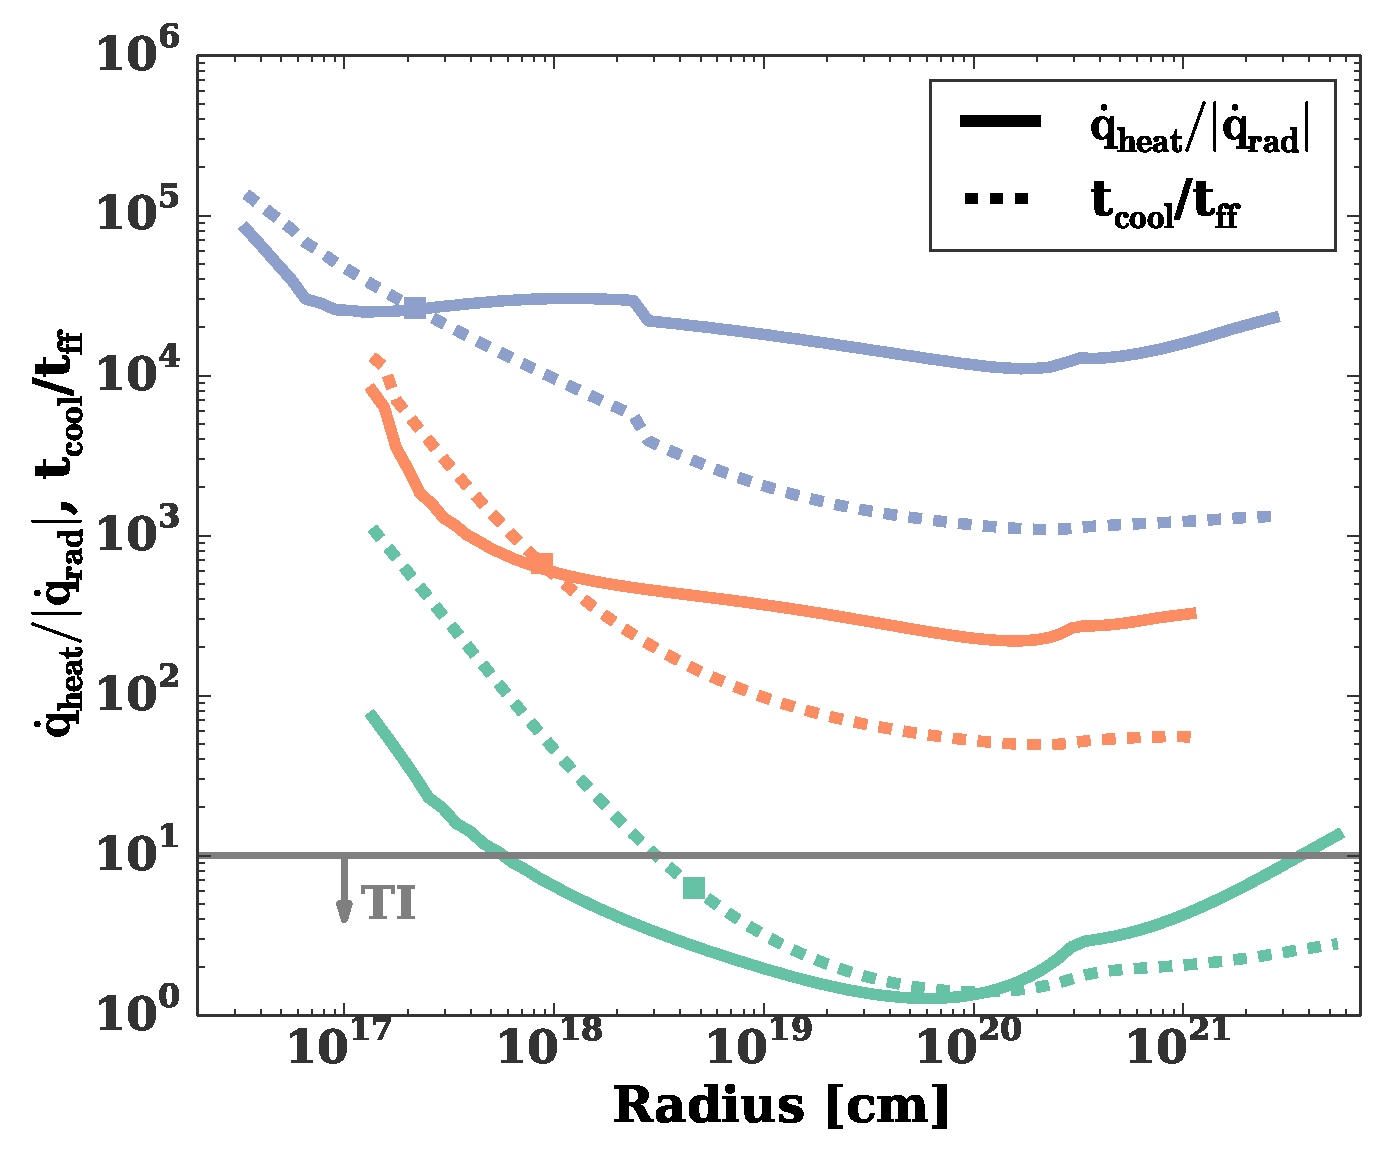
\includegraphics[width=\columnwidth]{cooling.eps}
  \caption{\label{fig:cooling} Ratio of the rate of heating to radiative cooling, $\dot{q}_{\rm heat}/\dot{q}_{\rm cool}$, as a function of radius for each of our solutions (solid lines).  Shown for comparison with dashed lines is the ratio of the cooling to the local free-fall timescale $t_{\rm cool}/t_{\rm ff}$.  For high heating rates both ratios are approximately equal at the stagnation radius (marked with a square for each solution).  When $\dot{q}_{\rm heat}/\dot{q}_{\rm cool} \lesssim 1$ and $t_{\rm cool}/t_{\rm ff} \lesssim 10$ the flow will be susceptible to global and local thermal instability, respectively (e.g.,  \citealt{McCourt+12}).  {\bf BDM: change y axis labels to qdotheat/qdotcool, tcool/tff}.}
\end{figure}


%\begin{table}
\begin{tabular}{cccc}
\hline
Galaxy & $\eta_{\rm max}$ $v_{\rm w,0}=$200 km/s & $\eta_{\rm max}$ $v_{\rm w,0}=$500 km/s & $\eta_{\rm max}$ $v_{\rm w,0}=$1000 km/s \\
\hline
NGC1023 & 0.1 & 2.0 & 200.0 \\
NGC1316 &  &  &  \\
NGC4365 &  &  & 100.0 \\
NGC4239 &  &  &  \\
NGC2841 &  &  &  \\
NGC4387 & 0.3 & 90.0 & 5000.0 \\
NGC3115 & 0.2 & 0.7 & 30.0 \\
NGC4621 & 0.3 & 1.0 & 40.0 \\
NGC4564 & 0.1 & 4.0 & 700.0 \\
NGC7768 &  &  &  \\
NGC4464 & 0.3 & 20.0 & 2000.0 \\
NGC4467 & 1.0 & 100.0 & 6000.0 \\
NGC1400 &  &  &  \\
NGC1399 &  &  &  \\
A2052 & 0.02 & 2.0 & 700.0 \\
NGC596 & 0.08 & 9.0 & 1000.0 \\
NGC4889 &  &  &  \\
NGC4472 &  &  &  \\
NGC224 & 0.02 & 4.0 &  \\
NGC5813 & 0.01 &  &  \\
NGC221 & 0.02 & 20.0 & 2000.0 \\
NGC2636 &  &  &  \\
NGC4486b & 0.005 & 0.1 & 50.0 \\
NGC720 &  &  &  \\
NGC1426 & 0.1 & 20.0 & 1000.0 \\
NGC3605 & 0.2 & 80.0 & 5000.0 \\
NGC4434 & 0.07 & 50.0 & 3000.0 \\
NGC4168 &  & 6.0 & 700.0 \\
NGC4636 &  &  &  \\
NGC3608 &  &  &  \\
NGC4551 & 0.1 & 50.0 & 3000.0 \\
NGC4552 &  &  &  \\
NGC4742 &  & 20.0 & 800.0 \\
NGC4478 & 0.03 & 40.0 & 3000.0 \\
NGC4570 & 0.2 & 4.0 & 400.0 \\
NGC4697 & 0.2 & 7.0 & 900.0 \\
NGC1172 &  & 20.0 & 1000.0 \\
NGC4458 & 0.03 & 30.0 & 2000.0 \\
NGC3599 & 0.8 & 200.0 & 9000.0 \\
NGC4874 &  &  &  \\
NGC3377 & 0.02 & 1.0 & 400.0 \\
NGC3379 & 0.02 &  & 200.0 \\
NGC2832 &  &  &  \\
NGC1700 &  &  &  \\
NGC1600 &  &  &  \\
NGC6166 &  &  &  \\
NGC4649 &  &  &  \\
NGC4486 &  & 0.02 &  \\
NGC524 &  &  &  \\
NGC7332 & 0.2 & 20.0 & 2000.0 \\
NGC5845 & 0.06 & 0.3 & 50.0 \\
\end{tabular}
\hline
\end{table}



\section{Numerical Results}
\label{sec:numerical}

\begin{table*}
\centering
\begin{minipage}{18cm}
\caption{Summary of Numerical Solutions}
\begin{tabular}{lccccccccccccc}
\hline
{$M_{\bullet,8}$} & {$v_{w}$} & {$\Gamma^{(a)}$} & {$r_b$} & {$\dot{M}/\dot{M}_{\rm edd}$} & {$(t_{\rm cool}/t_{\rm ff})_{r_s}$} & {comments}\\
\hline
0.01 & 300 & 0.8 & U & $ 3.2 \times 10^{ -4 }$ & 4.7 & rb in fact
unresolved \\
0.01 & 600 & 0.8 & U & $ 5.5 \times 10^{ -5 }$ & $ 3.2 \times
10^{ 2 }$ &  \\
0.01 & 1200 & 0.8 & U & $ 9.4 \times 10^{ -6 }$ & $ 1.5 \times
10^{ 4 }$ &  \\
0.1 & 300 & 0.8 & 100.0 & $ 2.5 \times 10^{ -3 }$ & 0.29 & \\
0.1 & 600 & 0.8 & 100.0 & $ 1.8 \times 10^{ -4 }$ & 97 &  \\
0.1 & 1200 & 0.8 & U & $ 3.1 \times 10^{ -5 }$ & $ 4.8 \times
10^{ 3 }$ &  \\
1 & 300 & 0.8 & 100.0 & $ 1.6 \times 10^{ -2 }$ & $ 5.6 \times 10^{
  -2 }$ &  TI\\
1 & 600 & 0.8 & 100.0 & $ 7.3 \times 10^{ -4 }$ & 21 &  \\
1 & 1200 & 0.8 & 100.0 & $ 9.9 \times 10^{ -5 }$ & $ 1.5 \times 10^{
  3 }$ &  \\
1 & 300 & 0.8 & 50.0 & $ 8.2 \times 10^{ -3 }$ & 0.19 &  \\
1 & 300 & 0.8 & 200.0 & $ 3.6 \times 10^{ -2 }$ & $ 1.7 \times 10^{
  -2 }$ &  TI/convergence \\
%1 & 300.0 & 0.8 & 300.0 & $ 5.2 \times 10^{ -2 }$ & $ 9.8 \times 10^{
%  -3 }$ &  TI/convergence\\
1 & 300 & 0.8 & 400.0 &  &  &  TI/run unsuccessful\\
0.1 & 300 & 0.8 & 50.0 & $ 2.0 \times 10^{ -3 }$ & 0.46 &  \\
0.1 & 300 & 0.8 & 200.0 & $ 5.3 \times 10^{ -3 }$ & 0.12 &  TI/convergence\\
%0.1 & 300.0 & 0.8 & 300.0 & $ 7.2 \times 10^{ -3 }$ & $ 6.7 \times
%10^{ -2 }$   & TI/convergence  \\
0.1 & 300 & 0.8 & 400.0 & $ 8.9 \times 10^{ -3 }$ & $ 4.7 \times
10^{ -2 }$ & TI/convergence \\
0.01 & 1200 & 0.1 & N/A & $ 1.5 \times 10^{ -6 }$ & $ 4.1 \times
10^{ 4 }$ &  rb is unsresolved\\
0.1 & 1200 & 0.1 & N/A & $ 9.5 \times 10^{ -6 }$ & $ 5.7 \times 10^{
  3 }$ &  tried run in which rb=100 pc was resolved what would happen if rb=400 pc?\\
0.01 & 1200 & 0.1 & 100.0 & $ 1.5 \times 10^{ -6 }$ & $ 4.1 \times 10^{ 4 }$ &  \\
0.1 & 1200& 0.1 & 100.0 & $ 9.5 \times 10^{ -6 }$ & $ 5.7 \times 10^{ 3 }$ &  \\
1 & 1200 & 0.1 & 100.0 & $ 6.0 \times 10^{ -5 }$ & $ 8.6 \times 10^{ 2 }$ &  \\
1 & 1200 & 0.1 & 50.0 & $ 4.9 \times 10^{ -5 }$ & $ 1.2 \times 10^{ 3 }$ &  \\
1 & 1200 & 0.1 & 200.0 & $ 1.0 \times 10^{ -4 }$ & $ 3.4 \times 10^{ 2 }$ &  \\
%1 & 1200.0 & 0.1 & 300.0 & $ 1.9 \times 10^{ -4 }$ & $ 1.3 \times 10^{ 2 }$ &  convergence\\
1 & 1200 & 0.1 & 400.0 & $ 1.8 \times 10^{ -2 }$ & 0.37 &  TI/convergence\\
\hline
\label{table:models}  
\end{tabular}
$^{(a)}$ Inner power-law index of stellar Nuker profile.  $^{(b)}$
Break radius of stellar Nuker profile.  For profiles marked U, the
break radius is not resolved on the grid.
\end{minipage}
\end{table*}



This section describes the results of our numerical calculations,
which we use to assess the validity of the analytic expressions
provided in the previous section.  Numerical solutions are calculated
for each galaxy for three different values of the stellar wind heating
parameter $v_{w}$ = 300, 600, 1200 km s$^{-1}$.  In cases when the stagnation radius become very large and was difficult to resolve on the grid, we conclude that such solutions will be thermally unstable and terminated their calculations (these are marked as `thermally unstable' in the tables.  

Figure~\ref{fig:profiles} shows profiles of the density $\rho(r)$,
temperature $T(r)$, and radial velocity $|v(r)|$, for the cusp
($\Gamma=0.8$) solutions within our grid.  As expected, the gas
density increases towards the SMBH $\rho\propto r^{-n}$ with
$n\simeq1$, i.e. shallower than the $-3/2$ power law for
Bondi accretion. This power law behavior does not extend
through all radii, however, as the gas density profile has a break coincident
with the location of the break in the stellar light profile ($\rb=100$
pc). The temperature profile is relatively flat at large radii, but
increases as $\propto 1/r^{k}$ interior to the sphere of influence,
where $k$ is smaller than 1--the power expected for virialized gas within the black hole sphere of influence.
The inwardly directed velocity increases towards the hole with a profile that is somewhat steeper than the local free-fall velocity $v \propto v_{\rm ff}\propto r^{-1/2}$.
% {\bf BDM: I made this up - in general we need
%   more explanation of what the plots are actually showing, with some
%   physical explanation.}
% AG -- things are not quite approaching Bondi on the inner grid. I
% don't have a good physical explanation yet...


Figure~\ref{fig:stag} shows our results for the
stagnation radius $r_{\rm s}$, expressed in ratio to the radius of the
SMBH sphere of influence $r_{\rm soi}$, with different colors showing
different values of $v_{w}$.  Cusp and core galaxies are marked with
square and triangles, respectively.  

 We may also compare our numerical results $r_{\rm s}/r_{\rm
  soi}$ an be compared directly to our analytic estimate in equation
\ref{eq:stag_analytic}.  The solid and dashed black curves in  Figure
\ref{fig:stag} show the analytic results for $r_{\rm s}/r_{\rm soi}$.
The good agreement provides a useful check of the numerical
results. Note that the analytic curves implicitly assume a density
slope, $n$ at $\rs$, which we have fixed to be 1 (0.5) for the solid
(dashed) curve. For small $\vw/\sigma$ this assumption breaks down.

For $\vw/\sigma \gg 1$ the value $\rs/\rsoi$ does not depend on break
radius, $r_b$. On the other hand for $\vw/\sigma \simeq 1$, $\rb$ does
have an effect. Notice that near where the solid analytic curve
diverges there are three green square, one over the other. These
points correspond to models with the same $\Mbh (10^7 \Msun)$, $\vw
(300 {\rm km/s})$, and $\Gamma (0.8)$, but different values of the
break radius: from top to bottom 50 pc, 100 pc, and 400 pc.  
%% AG: Describe conservation checks to additionally validate the results.

\begin{figure}
  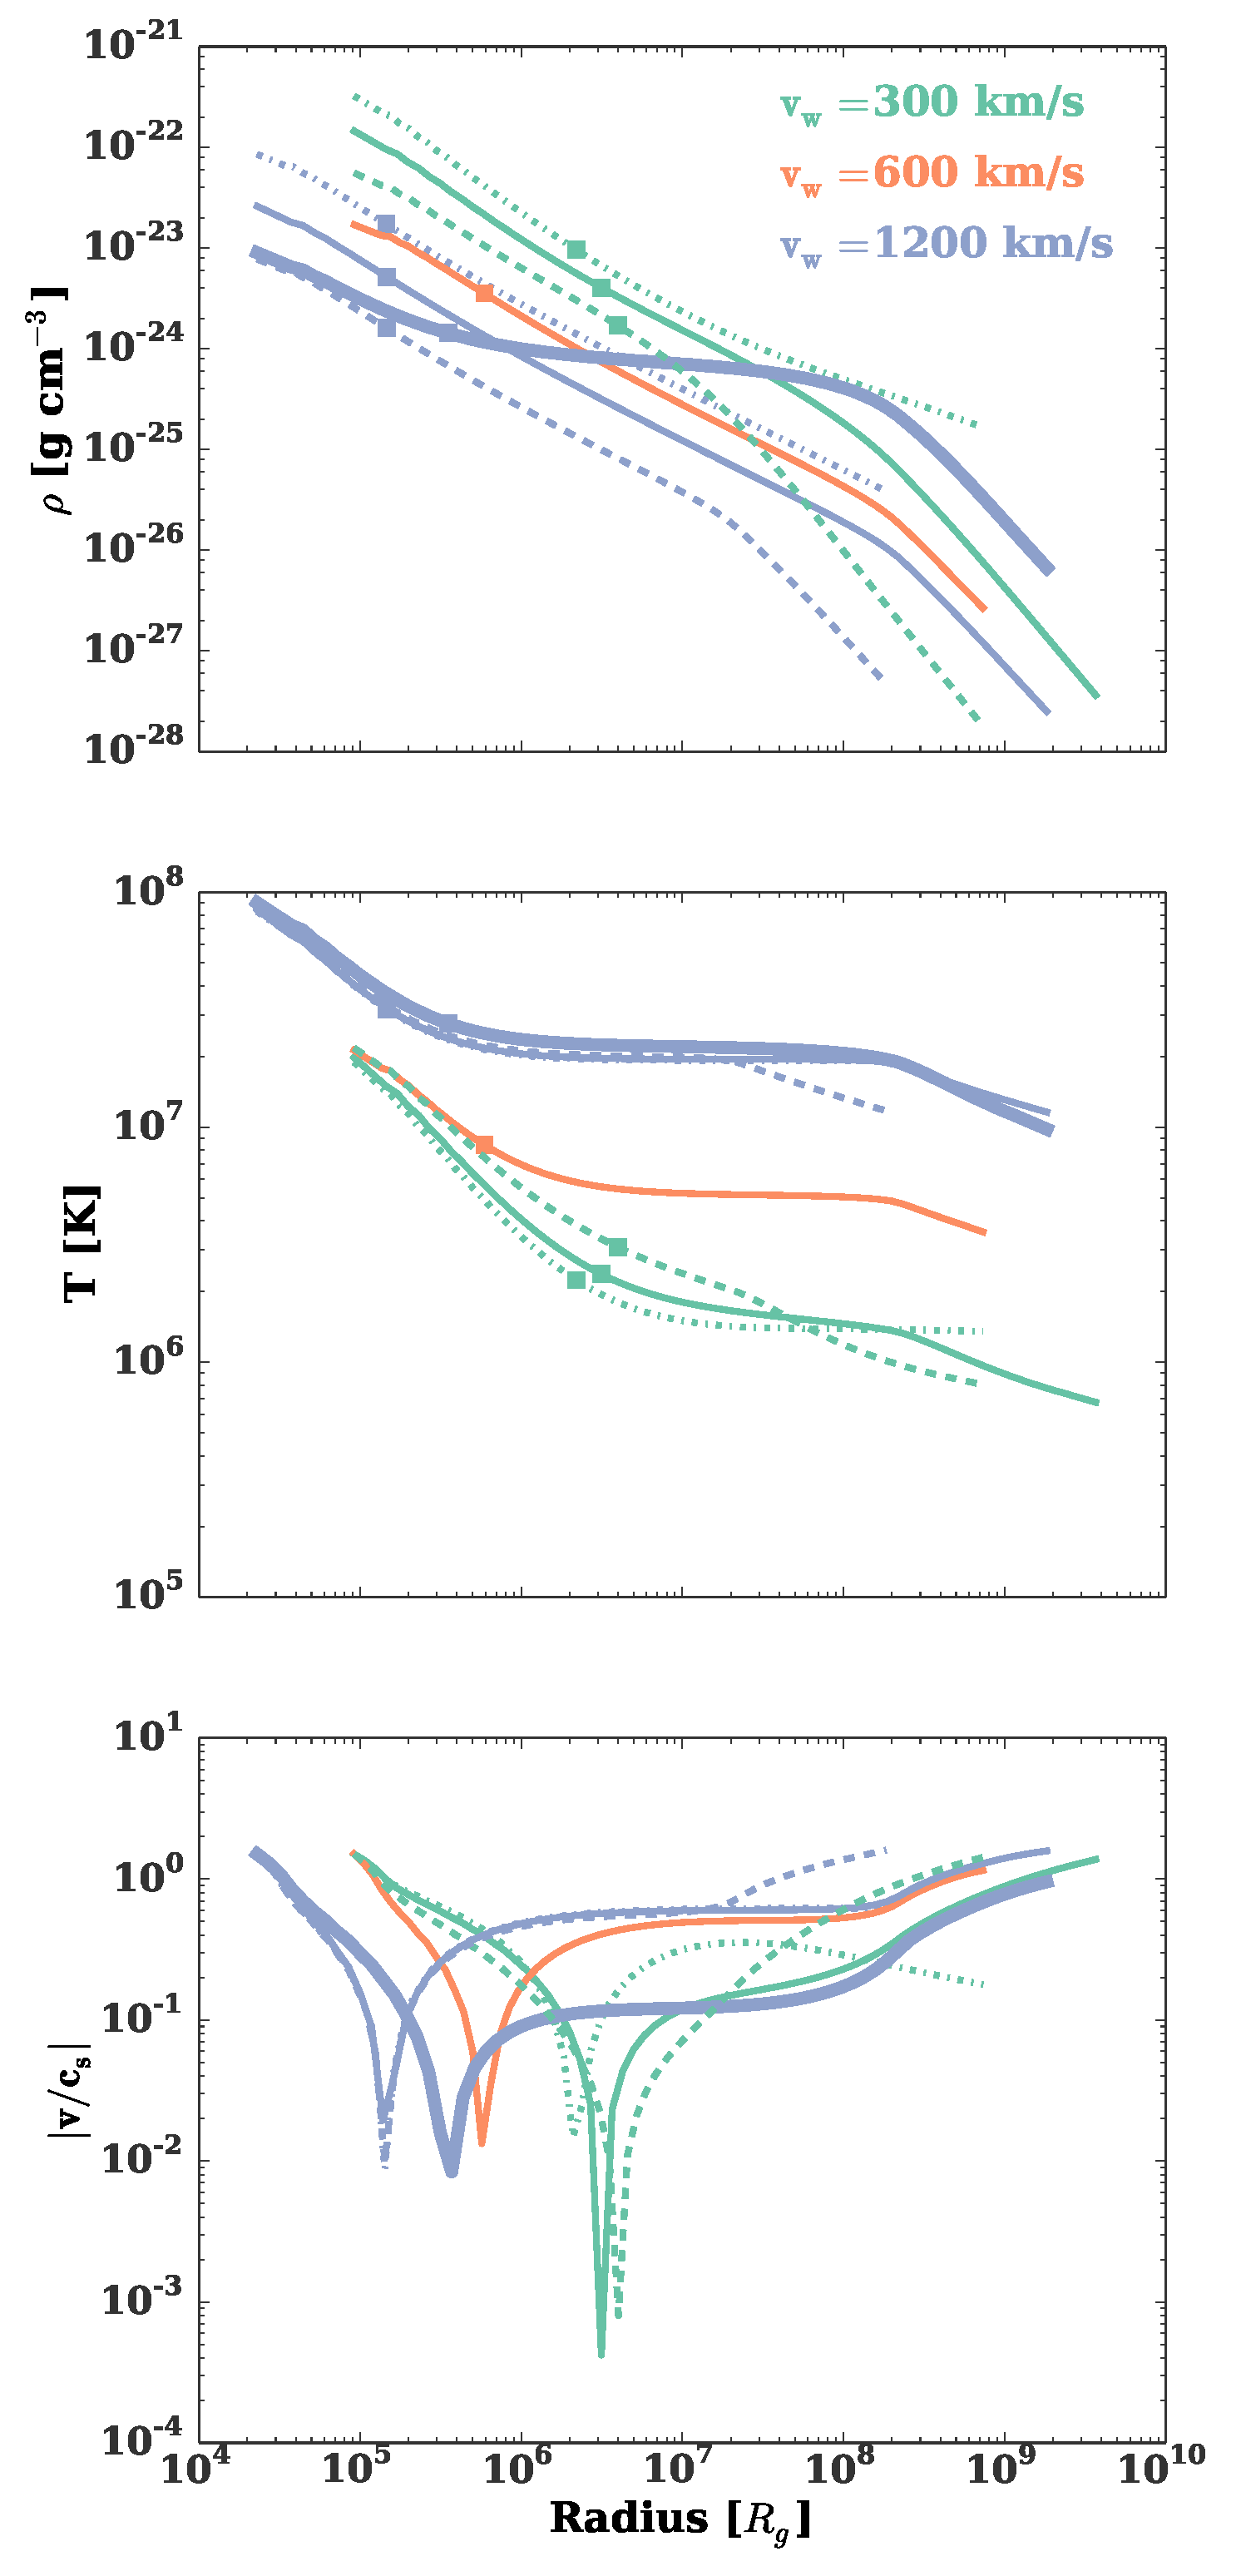
\includegraphics[width=\columnwidth]{profiles.eps}
  \caption{\label{fig:profiles}Radial profiles of the CNM density
    ({\it top}), temperature ({\it middle}), velocity ({\it bottom}),
    and interior X-ray luminosity ({\it bottom}) calculated for a
    sample of galaxies within our grid.  Different colors
    denote different values of the effective wind heating rate,
    $\vwO=1200$ km s$^{-1}$ ({\it blue}), $\vwO$=600 km s$^{-1}$ ({\it
      orange}), and 300 km s$^{-1}$ ({\it green}).  Different
    linestyles correspond to different values of $\Mbh$, $\Mbh=10^6
    \Msun$ ({\it dot-dashed}), $\Mbh=10^7 \Msun$ ({\it solid}), and
    $\Mbh=10^8 \Msun$ ({\it dashed}). Thin lines correspond to cusp
    galaxies ($\Gamma$=0.8) and thick lines correspond to core
    galaxies ($Gamma$=0.1). Squares mark out the location of
    the stagnation radius for each solution.
 }
\end{figure}

\begin{figure}
  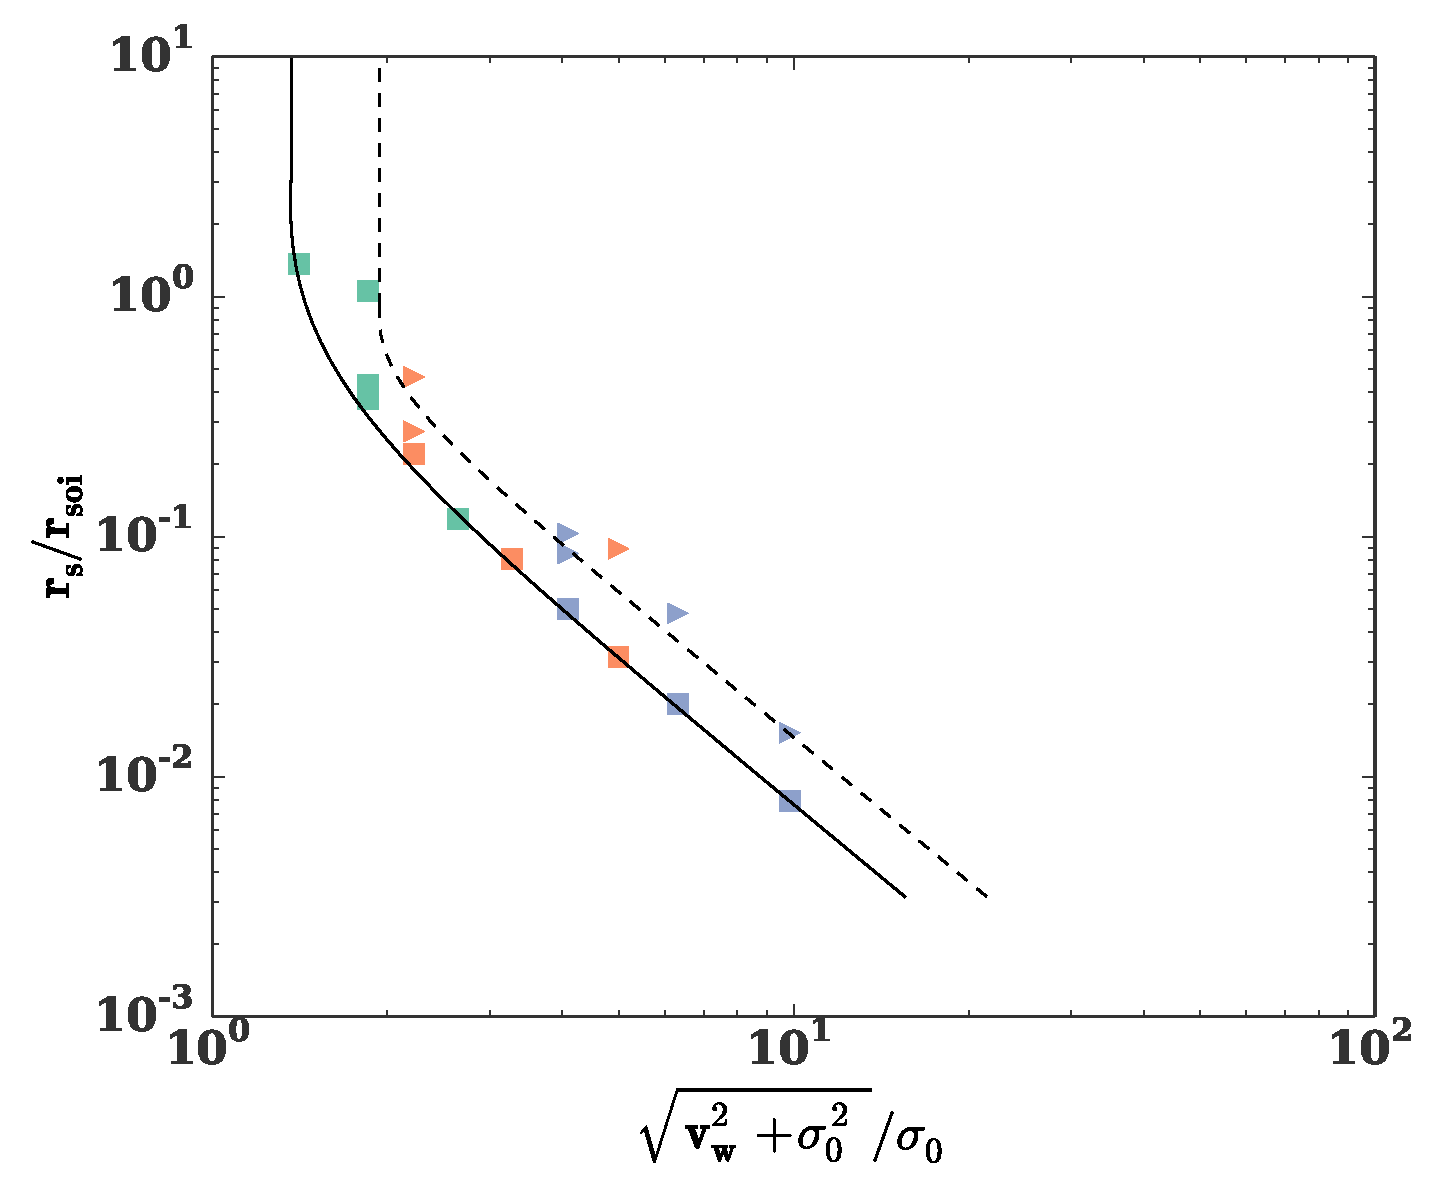
\includegraphics[width=\columnwidth]{rs.eps}
  \caption{\label{fig:stag} \emph{Top panel:} Stagnation radius
    $r_{s}$ (in units of the radius of the sphere of influence $r_{\rm
      soi} = GM_{\bullet}/\sigma^{2}$) for galaxies in our sample as a
    function of the ratio of the effective wind heating rate $v_{w}$
    to the stellar velocity dispersion $\sigma$.  Green, orange, and
    blue symbols represent $v_{w} =$ 300, 600, and 1200 km s$^{-1}$,
    respectively.  Squares correspond to cusp galaxies, while
    triangles correspond to cores. The black curves correspond to the
    analytic prediction from Equation~\eqref{stag_analytic}. The solid
    (dashed) curve is the correponds to $\Gamma=0.8$ and $n=1$
    ($\Gamma=0.1$ and $n=0.5$.}
\end{figure}


Fig.~\ref{fig:cooling} shows $H/C=\frac{1}{2} (q \vw^2+q
v^2)/\left|\Lambda(T) n^2\right|$ and $\tcool/\tff$
as a function of radius for all of our solutions. {\bf BDM: change
  plots}, with different colors denoting different values of $\vwO$.
For our highest heating rates we observe that cooling is unimportant
for all solutions across all radii--neither the local nor the global
thermal instability would be present. However,  for our smallest value
of $\vwO$=300 km s$^{-1}$ with $\Mbh=10^8 \Msun$, the solution would be
thermally unstable as $H/C<1$ and $\tcool/\tff<10$. Note that the
precise region of the parameter space which would be thermally
unstable would depend on the value of $\eta$--in
Fig.~\pageref{fig:cooling} we have chosen $\eta=0.02$, which would be
appropriate for a stellar population with $\tage\simeq \th$. This
value is on the low end of what we would physically expect for
$\eta$. 

For $\vwO=1200$ km s$^{-1}$ and $\vwO=600$ km s$^{-1}$, we have
$H/C\simeq\tcool/\tff$ at $\rs$ as expected. However, the two ratios
diverge away from $\rs$, as equation~\eqref{eq:rhors2} is not a good
approximation away from $\rs$. Similarly, it is poorer approximation
for $\vwO=300$ km s$^{-1}$. Hence, $H/C$ and $\tcool/\tff$ do not
closely match at $\rs$ for this $\vwO$. {\bf AG would be good to
  clarify the physics here a little more.}

\section{Sources of Heating}
\label{sec:heating}

Key properties of the flow, such as the stagnation radius, the SMBH accretion rate, and the likelihood of thermal instability depend sensitively on the assumed heating rate $\propto qv_{w}^{2}$.  This section summarizes individual heating sources, providing estimates of the value of
\begin{align}
  v_{w} = \sqrt{\frac{2 t_h e}{\eta \rhostar}}
  \label{eq:vw_eff}
\end{align}
for each, where $e$ is volumetric heating rate.  

\subsection{Stellar winds} 

Energy and mass input to the CNM by stellar winds is the sum of contributions from main sequence and post-main sequence stars.  At early times following star formation, energy input is dominated by core collapse supernovae and by the fast outflows of Wolf-Rayet stars, while at later times energy input is dominated by main sequence winds.  Mass input is also dominated by massive stars for very young stellar populations, but for most stellar ages mass input is dominated by the slow AGB winds of low mass stars.  

Appendix \ref{app:windheat} provides a calculation of wind heating rate from stellar winds, $v_{\rm w}^{\star}$, and the mass loss parameter, $\eta$ (eq.~[\ref{eq:q}]), as a function of age $\tau_{\star}$ of a stellar population which is formed impulsively (Figs.~\ref{fig:vwimp}, \ref{fig:etaImp}).  At very early times after the starburst ($\tau_{\star} \lesssim 10^{7}$), the wind heating rate exceeds 1000 km s$^{-1}$, while at much later times ($\tau_{\star} \sim t_{\rm h}$) stellar wind heating is much lower, $v_{\rm w} \sim 50 $ km s$^{-1}$ (see also \citealt{NaimanSoares-Furtado+:2013a}).  As we describe in $\S$, the net heating rate produced by stellar winds in the case of quasi-continuous star formation, as representative of the average star formation history of low mass galaxies, can also be significant, $v_{\rm w}^{\star} \gtrsim 1000$ km s$^{-1}$.  Thus stellar winds contribute a potentialy important source of energy as well as mass for the CNM.

\subsection{Type Ia Supernovae} 

Type Ia supernovae (SNe Ia) represent a potentially important source of heating, which unlike core collapse SNe is present even in an evolved stellar population.  If each Ia supernova injects thermal energy $E_{\rm Ia}$ into the interstellar medium, and the SNe rate (per stellar mass) is given by $R_{\rm   Ia}$, then the resulting volumetric heating rate $E_{\rm Ia}R_{\rm  Ia}$ produces an effective wind heating parameter (equation~[\ref{eq:vw_eff}]) \begin{align} v_{w}^{\rm Ia} =\sqrt{\frac{2 t_h R_{\rm Ia}
E_{\rm Ia}}{\eta}} \label{eq:vw_sne}.
\end{align} The thermal energy injected by a Ia SN $E_{\rm Ia} \simeq
\epsilon_{\rm Ia} 10^{51}$ ergs depends on the efficiency $\epsilon_{\rm Ia}$
with which the initial blast wave energy is converted into bulk or turbulent
motion instead of being lost to radiation.  \cite{Thornton+98}
estimate a radiative efficiency $\epsilon_{\rm Ia} \sim 0.1$,
depending weakly on surrounding density, but \citet{Sharma+14} argues
that $\epsilon_{\rm Ia}$ can be considerably higher, $\sim 0.4$, if
the SNe occur in a hot dilute medium, as may characterize the circumnuclear medium.  Hereafter we adopt $\epsilon_{\rm Ia} = 0.4$ as fiducial.

The Ia SN rate $\RateIa$ depends on the age of the stellar population, as it represent the convolution of the star formation rate and the Ia delay time distribution (DTD) divided by the present stellar mass.  In
the limit of impulsive star formation, $\RateIa$ is the DTD evaluated at the time since the star formation episode.  The observationally inferred DTD (Fig. 1 of \citealt{MaozMannucci+:2012a}) has the
approximate functional form \begin{align}
  R_{\rm Ia} =1.7\times 10^{-14}\left(\tau_{\star}/t_{\rm
      h}\right)^{-1.12} M_{\odot}^{-1}\,{\rm yr^{-1}}
\label{eq:DTD}
  \end{align}
  where $\tau_{\star}$ is the time since star formation
  (c.f.~\citealt{Scannapieco&Bildsten05}). 

From equations (\ref{eq:vw_sne}), (\ref{eq:DTD}) we thus estimate that 
  \begin{eqnarray} 
    v_{w}^{\rm Ia} &\approx& 700(\epsilon_{\rm
      Ia}/0.4)^{0.5}(\tau_{\star}/t_{\rm h})^{-0.56}\eta_{0.02}^{-1/2}\,{\rm km
      \,s^{-1}} \nonumber \\
&\approx& 700(\epsilon_{\rm
      Ia}/0.4)^{0.5}(\tau_{\star}/t_{\rm h})^{0.09}\,{\rm km
      \,s^{-1}},
\label{eq:vIa}
  \end{eqnarray}
where the second line assumes $\eta\simeq 0.02 (\tau_{\star}/t_h)^{-1.3}$ for a single burst of star formation (\citealt{Ciotti+91}).

The high value of $v_{w}^{\rm Ia}$ implies that Ia SNe represent an important source of CNM heating.  However, SNe can only be approximated as supplying constant heating throughout space and time if the rate of SNe is rapid compared to the inflow time at the radius of interest (\citealt{ShcherbakovWong+:2014a}).  We define the ``Ia radius"
  \begin{align}
    r_{\rm Ia} \sim \left(\frac{G}{R_{\rm Ia}\sigma}\right)^{1/2} \sim
    38 M_{\bullet,8}^{-0.1}(\tau_{\star}/t_{\rm h})^{0.56}\,{\rm pc}
    \label{eq:rIa}
  \end{align}
as the location exterior of which the time interval between subsequent supernovae $\tau_{\rm Ia} \sim (M_{\rm enc}R_{\rm Ia})^{-1} \sim G/(r\sigma^{2}R_{\rm Ia})$ exceeds the local dynamical timescale $t_{\rm
dyn} \sim r/\sigma$, where we again adopt the Ia rate for an old stellar population and in the final equality we estimate the velocity dispersion using the $M_{\bullet}-\sigma$ relationship
(equation~[\ref{eq:Msigma}]).  

Assuming that $v_{w}^{\rm Ia} \gg \sigma$ then by substituting $v_{w}^{\rm Ia}$ (eq.~\ref{eq:vIa}) into equation (\ref{eq:rs_simple}) for the stagnation radius, we find that
\begin{eqnarray}
\left.\frac{r_{\rm Ia}}{r_{\rm s}}\right|_{\rm v_{w}^{\rm Ia}} &\approx& 12.4\eta_{0.02} M_{\bullet,8}^{-1.1}(\epsilon_{\rm Ia}/0.4)^{-1}(\tau_{\star}/t_{\rm h})^{1.68} \nonumber \\
&\approx& 12.4M_{\bullet,8}^{-1.1}(\epsilon_{\rm Ia}/0.4)^{-1}(\tau_{\star}/t_{\rm h})^{0.38}
\label{eq:rIars}
\end{eqnarray}
The fact that $r_{\rm Ia} \gg r_{\rm s}$ appears to imply that Ia heating can only be approximated as a steady heating source near the stagnation radius for extremely massive SMBHs $M_{\bullet} \gtrsim 10^9 \Msun$ or very young populations ($\tau_{\star} \ll t_{\rm h}$).  However, equation (\ref{eq:rIars}) may underestimate the importance of Ia heating because $r_{\rm Ia}/r_{\rm s}$ will be substantially smaller than its value estimated using $v_{w}^{\rm Ia}$ if the nominal heating rate (without Ia contribution) is much less than this.  Nevertheless, the impact of Ia SN is clearly greater for larger SMBH masses for which $r_{\rm Ia} \lesssim r_{\rm s}$.

What is the effect of the Ia radius?  Between subsequent supernovae, stars release a gaseous mass $M_{\rm g} \approx \eta M_{\star}\tau_{\rm Ia}/t_{\rm h}$ interior to the Ia radius, which is gravitationally bound to the SMBH by an energy $E_{\rm bind} \sim M_{\rm g}\sigma^{2}$.  Thus, according to the above definitions, $E_{\rm Ia}/E_{\rm bind} \sim (v_{w}^{\rm Ia})^{2}/2\sigma^{2} \gtrsim 1$.  Hence Ia SN can in principle dynamically clear out gas from radii $\sim r_{\rm Ia} \gtrsim r_{\rm s}$.  Thus, even in cases when $r_{\rm s} > r_{\rm Ia}$, the SMBH accretion rate is limited to the value set by substituting the Ia radius $r_{\rm Ia}$ (eq.~[\ref{eq:rIa}]) for $r_{\rm s}$ in the derivation of equation $\ref{eq:eddr_analytic}$, i.e.  
\begin{eqnarray}
\left.\frac{\dot{M}}{\dot{M}_{\rm edd}}\right|_{\rm max} &\approx& \frac{\eta M_{\bullet}}{\dot{M}_{\rm edd} t_{\rm h}}\left(\frac{R_{\rm Ia}}{R_{\rm soi}}\right)^{2-\Gamma} \approx \nonumber \\
 && \begin{cases}
    4.5 \times 10^{-4} M_{\bullet,8}^{-1.33}(\tau_{\star}/t_{\rm h})^{-0.2}
   & \text{core} \\
    2.2 \times 10^{-4} \Mbheight^{-0.84}(\tau_{\star}/t_{\rm h})^{-0.6}   & \text{cusp}.
  \end{cases}
  \label{eq:eddr_Ia}
\end{eqnarray}
{\bf AG: Changed this expression somewhat from that of BDM (slightly
  different scaling relations were used?). I will
  check again! Note that the time dependence of eta~t$^{-1.3}$ is
  folded in above.}


\subsection{Millisecond Pulsars}
 Energy injection from millisecond pulsars (MSPs) is a potentially
important heating source.  If the number of MSPs per unit stellar mass
is $n_{\rm msp}$ and each contributes on average a spin-down
luminosity $\bar{L}_{\rm sd}$, then the resulting heating per unit
volume $e \approx \bar{L}_{\rm sd}n_{\rm msp}\epsilon_{\rm msp}$ results in an
effective heating rate (eq.~ [\ref{eq:vw_eff}])
\begin{eqnarray} v_{w}^{\rm MSP} \approx
30\left(\frac{\epsilon_{\rm msp}}{0.1}\right)^{1/2}\left(\frac{\bar{L}_{\rm
sd}}{10^{34}\,{\rm erg\,s^{-1}}}\right)^{1/2} \eta_{0.02}^{-1/2}\,{\rm
km\,s^{-1}},
 \label{eq:vmsp}
  \end{eqnarray} 
where $\epsilon_{\rm msp}$ is the thermalization efficiency of
the wind, normalized to a value $\epsilon \lesssim 0.1$ inferred based
on modeling the insterstellar mediums of globular clusters
\citep{NaimanSoares-Furtado+:2013a}.  The above estimate adopts a
pulsar density $n_{\rm msp}\simeq3 \times 10^{-40} $ MSPs g$^{-1}$
motivated by the $\sim 30,000$ estimated MSPs in the Milky Way of
stellar mass $6\times 10^{10}M_{\odot}$ (\citealt{Lorimer13}).

The average spin-down luminosity of millisecond pulsars in the field
is estimated to be $\bar{L}_{\rm sd} \sim 10^{34}$ erg s$^{-1}$ based
on the ATNF radio pulsar catalog (\citealt{Manchester+05}), in which
case $v_{w} \lesssim 30$ km s$^{-1}$.  For higher spin-down
luminosities, $L_{\rm sd}\simeq 10^{35}$ ergs s$^{-1}$ characteristic
of some Fermi-detected pulsars, then the higher value of $v_{w}
\lesssim 300$ km s$^{-1}$ makes MSP heating in principle important
under the optimistc assumption $\epsilon_{\rm msp} = 1$.  On the other hand, the
binaries giving rise to MSPs may be disocciated by stellar
interactions in the dense nuclear cluster, reducing their numbers as
compared to the field population estimate above.  MSPs are thus unlikely to be an important source of heating in comparison to stellar heating.


\subsection{SMBH Feedback}

Feedback from accretion onto the SMBH represents an important source of heating which, however, is also the most difficult to quantify.  A key difference between AGN heating and the other sources discussed thus far is its dependence on the SMBH accretion rate $\dot{M}$, which is itself a function of the heating rate (eq.~[\ref{eq:mdot_analytic}]).  

There are two types of SMBH feedback: kinetic and radiative.  Radiative feedback is potentially effective even in low luminosity AGN via Compton heating, which provides a volumetric heating rate (\citealt{Gan+14})
\be
\dot{e}_{\rm C} = 4.1\times 10^{-35}n^{2}\xi T_{\rm C}\,{\rm erg\,cm^{-3}\,s^{-1}},
\ee
where $\xi = L/n r^{2}$ is the ionization parameter and $L$ is the SMBH luminosity with Compton temperature $T_{\rm C} \sim 10^{9}$ K $\gg T$ (\citealt{Gan+14}).  

{\bf AG: Note that the Compton heating will depend on the distance of
  the hole as $1/r^2$ so Compton heating will be stronger closer to the
  black hole! }
The importance of Compton heating can be estimated by assuming the SMBH
radiates with a luminosity $L = \epsilon_{\rm rad} \dot{M}c^{2}$, where
$\epsilon_{\rm rad}$ is the radiative efficiency and where $\dot{M}$ is
estimated from equation (\ref{eq:mdot_analytic}).  Then using
equations (\ref{eq:rs_simple}), (\ref{eq:mdot_analytic}),
(\ref{eq:rhors}), (\ref{eq:rhostarrs}) we calculate that from equation
(\ref{eq:vw_eff}) that the effective Compton heating rate at the stagnation radius is given by
\begin{align} v_{w}^{\rm C} \simeq
  \begin{cases} 29 \eta_{0.02}^{0.5}T_{\rm
C,9}^{0.5}\epsilon_{-2}^{0.5} M_{\bullet,8}^{0.38}v_{500}^{-1.4}\,{\rm
km\,s^{-1}} &, \text{core}\\ 50 \eta_{0.02}^{0.5}T_{\rm
C,9}^{0.5}\epsilon_{-2}^{0.5} M_{\bullet,8}^{0.24}v_{500}^{-0.7}\,{\rm
km\,s^{-1}} &, \text{cusp},
  \end{cases}
  \label{eq:vC}
\end{align} where $T_{C,9} = T_{C}/10^{9}$ K and $\epsilon_{-2} =
\epsilon_{\rm rad}/0.01 \sim 1$ is the maximum radiative efficiency
for an advective accretion flow expected to produce high $T_{\rm C}$
emission (e.g.~\citealt{Narayan&Yi95}).  If heating is provided by
Compton heating alone, i.e. $\tilde{v}_{w} = v_{w}^{C}$, then equation
(\ref{eq:vC}) can be solved for $\tilde{v}_{\rm w}$ to find
\begin{align} v_{w}^{\rm C} \simeq
  \begin{cases} 106 \eta_{0.02}^{0.21}T_{\rm
C,9}^{0.21}\epsilon_{-2}^{0.21} M_{\bullet,8}^{0.16}\,{\rm km\,s^{-1}}
&, \text{core}\\ 76 \eta_{0.02}^{0.29}T_{\rm
C,9}^{0.29}\epsilon_{-2}^{0.29} M_{\bullet,8}^{0.14}\,{\rm km\,s^{-1}}
&, \text{cusp},
  \end{cases}
  \label{eq:vC2}
\end{align} 
The fact that $v_{w}^{\rm C} \lesssim 200$ km s$^{-1}$ for physically realized values of $\eta \lesssim 1$ shows that Compton heating alone is insufficient to stabilize the flow against cooling
instability, i.e. $v_{w}^{C} < v_{\rm CI}$ (eq.~[\ref{eq:cooling2}]).

Kinetic feedback occurs from an outflow of mass or energy  from the viscinity of the black hole in the form of a disk wind or jet, which deposits its energy across a much wider range of radii.  If the total outflow power is proportional to the SMBH accretion rate, $L_{\rm j} = \epsilon_{\rm j} \dot{M}c^{2}$, where $\epsilon_{\rm j} < 1$ is an efficiency factor.  Assuming that this energy is deposited uniformly out to a radius $r_{\rm heat}$ and volume $V_{\rm heat} \propto r_{\rm heat}^{3}$, then the volumetric heating rate $e = \epsilon_{\rm j}\dot{M}c^{2}/V_{\rm heat}$ results in an effective wind velocity at the stagnation radius given by
\begin{eqnarray} v_{w}^{\bullet} &\approx& \left(\frac{2t_{\rm
h}\epsilon_{\rm j}\dot{M}c^{2}}{V_{\rm heat}\eta
\rho_{\star}}\right)^{1/2} \sim \left(\frac{\epsilon_{\rm
j}\dot{M}c^{2}t_{\rm h}}{\eta M_{\rm enc}}\right)^{1/2} \nonumber \\
&\approx& 300\,{\rm km\,s^{-1}}\,\left(\frac{\epsilon_{\rm j}}{10^{-6}}\right)^{1/2}\left(\frac{r_{\rm s}}{r_{\rm
heat}}\right)^{1-\Gamma/2},
\label{eq:vjet}
\end{eqnarray} where we have used the fact that $\dot{M} \approx \eta
M_{\rm enc}(r_{\rm s})/t_{\rm h}$ and that $M_{\rm enc}(r) \propto
M_{\bullet}(r/r_{\rm soi})^{2-\Gamma}$ for radii interior to the outer
break radius (eq.~[\ref{eq:rhostar}]).  Thus for $r_{\rm heat} \sim
r_{\rm s}$, even a modest heating efficiency $\epsilon_{\rm j} \gtrsim
10^{-5}$ is sufficient for $v_{w}^{\bullet}$ to exceed other
sources of non-accretion powered heating.  However, if the jet distributes its energy on much larger scales comparable to the size of the galaxy, i.e. $r_{\rm heat} \gtrsim $ kpc $\gtrsim 10^{3}r_{\rm s}$ then the heating rate would be much less significant, even for an efficient jet ($\epsilon_{\rm j} \sim 1$).

Also note that for a fixed $r_{\rm heat}$, the effective heating rate $v_{\rm  w}^{\bullet} \propto r_{\rm s}^{1-\Gamma/2} \propto M_{\bullet}^{1-\Gamma/2}v_{w}^{\Gamma-2}$ is proportional to $v_{w}$ to a negative power (where we have used of eq.~[\ref{eq:stag_simple}]).  This shows that SMBH kinetic heating, if dominant, could thus `self-regulate' insofar as a lower heating rate results in a higher accretion rate, which in turn results in stronger jet feedback.  Importantly, however, unlike in the case of local heating sources such as stellar winds, even a dominant SMBH heating may not allow for a thermally-stable steady flow because the central accretion rate does not respond instantaneously to changes in the
thermodynamic properties of the gas on larger scale.  We also note here that the kinetic heating rate is proportional to the SMBH mass to a positive power, $v_{w}^{\bullet} \propto M_{\bullet}^{1(0.5)}$ for core(cusp) galaxies, respectively. This dependence could have important implications for the dependence of the average nuclear X-ray luminosity of quiescent galaxies on the SMBH mass ($\S\ref{sec:mdot}$).

What is a physically motivated value of the heating radius $r_{\rm
  heat}$?  \citet{Bromberg+11} show that a jet of luminosity $L_{\rm
  j}$ and half opening angle $\theta_{\rm j} = 0.1$ (characteristic of
AGN jets) propagates through a gaseous mass $M_{\rm g}$ to a radius
$r$ in a timescale
\begin{eqnarray}
t_{\rm jet} &\sim& 4000\,{\rm yr}\left(\frac{{L}_{\rm j}}{10^{40}\,\rm erg\,s^{-1}}\right)^{-1/3}\left(\frac{r}{\rm pc}\right)^{2/3}\left(\frac{M_{\rm g}}{10^{8}M_{\odot}}\right)^{1/3} 
\end{eqnarray}
Writing $L_{\rm j} = \epsilon_{\rm j}\dot{M}c^{2}$ and approximating $M_{\rm g} \sim \dot{M}t_{\rm ff}$ we find that the ratio of the jet crossing time to the free-fall time $t_{\rm ff} \sim r/\sigma$ is 
\begin{equation}
\frac{t_{\rm jet}}{r/\sigma} \sim 8\times 10^{-5}\sigma_{200}^{2/3}\epsilon_{\rm j}^{-1/3},
\end{equation}
which is notably independent of radius $r$.  Thus we require $\epsilon_{\rm j} \gtrsim 10^{-12}$ for the jet to escape, and if it escapes it is free to travel a long distance. 

\subsection{Combined Heating Rate} 

The total gas heating rate $\vwO$ includes contributions from stellar winds, supernovae, pulsars, and SMBH feedback.  The strength of each heating source will depend on the SMBH mass and the star formation history in the galactic nuclear region, the latter of which will vary systematically with the galaxy mass and hence with $\Mbh$.  Qualitatively, smaller galaxies will on average have more recent star formation, resulting in energetic young stellar winds and supernovae which dominate the energy budget, resulting in a high heating rate of $\vwO \sim 1000 $ km s$^{-1}$.  Larger galaxies, on the other hand, will on average have older stellar populations, with their heating rates dominated by Ia supernovae (on large radial scales) and SMBH feedback.

The average star formation history as a function of $\Mbh$ and the $\vwO$ for each heating source is estimated by using the average cosmic star formation histories determined by \citet{MosterNaab+:2013a}.  As described in detail in Appendix \ref{app:windheat}, the average star formation history is used to estimate the stellar wind heating $v_{\rm w}^{\star}$ and the mass input parameter $\eta$ (Fig.~\ref{fig:eta}), the latter of which affects the other sources of feedback, including AGN ($v_{\rm w}^{\bullet}$; eqs.~[\ref{eq:vC}], [\ref{eq:vjet}]), millisecond pulsars ($v_{w}^{\rm msp}$; eq.~[\ref{eq:vmsp}]), and Ia supernovae ($v_{w}^{\rm Ia}$; eq.~[\ref{eq:vIa}]), the latter of which also depends on a convolution of the star formation history and the Ia delay-time distribution (eq.~[\ref{eq:DTD}])

Figure~\ref{fig:vwSources} shows $\vwO$ from each heating source (stars, MSPs, SNe Ia, and black hole
feedback) as a function of black hole mass.  MSP heating is found to be negligible at all black hole masses.  The young stellar populations in galaxies with $\Mbh\lsim 10^{7.5} \Msun$ results in $v_{w}^{\star}$ being dominant.  For $\Mbh\gsim 10^{7.5} \Msun$ , the younger stellar population with their energetic
stellar winds is dead, and Compton heating plays an important role.


\begin{figure}
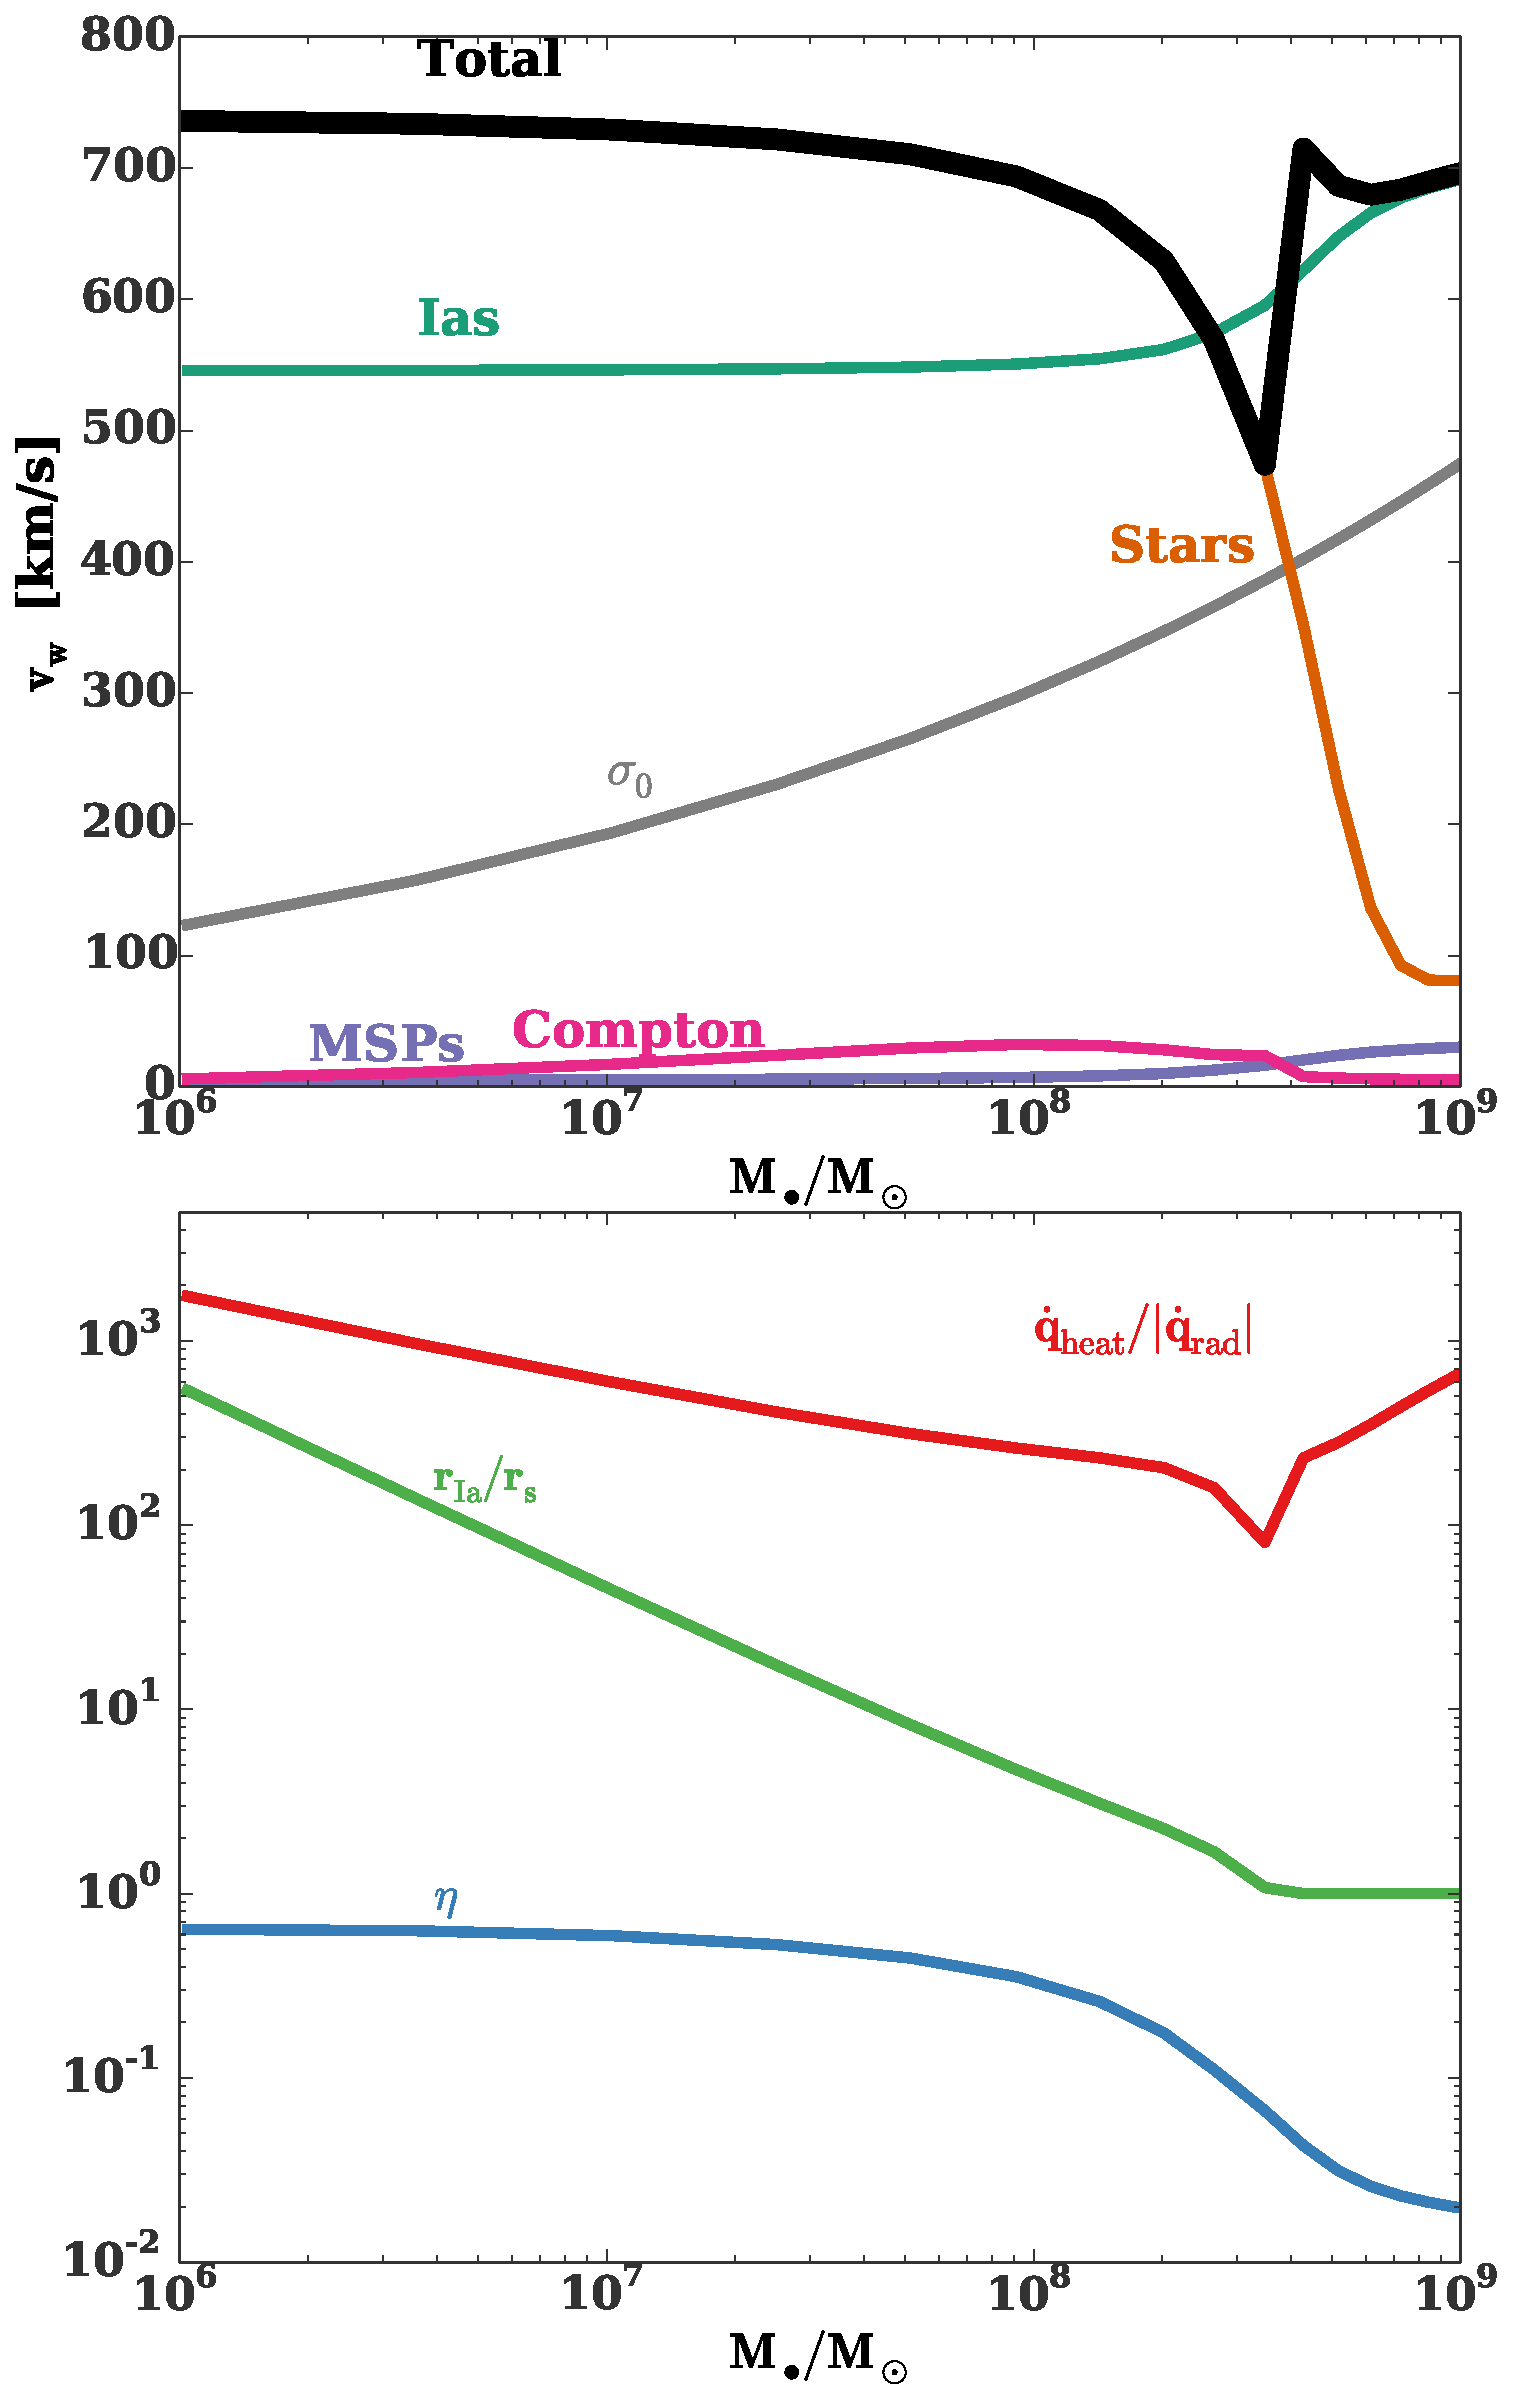
\includegraphics[width=\columnwidth]{vwSources.pdf}
\caption{\label{fig:vwSources} {\emph Top Panel:}Sources contributing
  to the heating rate of the CNM, $\vwO$, including stellar wind
  heating ({\it orange}), Ia supernovae ({\it green}), millisecond
  pulsars ({\it blue}), and compton heating (\it pink).  Each heating
  source varies with black hole mass $\Mbh$ due to the different
  average star formation history of galaxies of a given halo mass (see
  Appendix~\ref{app:windheat} for the detailed description). The total
  heating rate is shown in black. To account for the non-steady nature
  of the Ia heating we multiply the Ia heating by $e^{-\rs/\rIa}$, so
  the contribution that the heating contribiution from Ia supernovae
  will be suppressed if the time between successive supernovae is much
  greater than the dynamical time at $\rs$. {\emph Bottom panel} The
  ratio of the heating ($\dot{q}_{\rm heat}$) to the cooling rate
  ($\dot{q}_{\rm cool}$) at $\rs$ from the total heating rate in the
  top panel. Above $\Mbh\simeq 5\times 10^7 \Msun$ $\dot{q}_{\rm
    heat}(\rs)<\dot{q}_{\rm cool}(\rs)$ and a thermal instability
  would arise. The thermally unstable region is marked in red in the
  bottom panel. All curves become dashed in the thermally unstable
  region of parameter space: we expect our model to break down in this
  regime as the steady-state assumption would be violated.}
\end{figure}


\begin{figure}
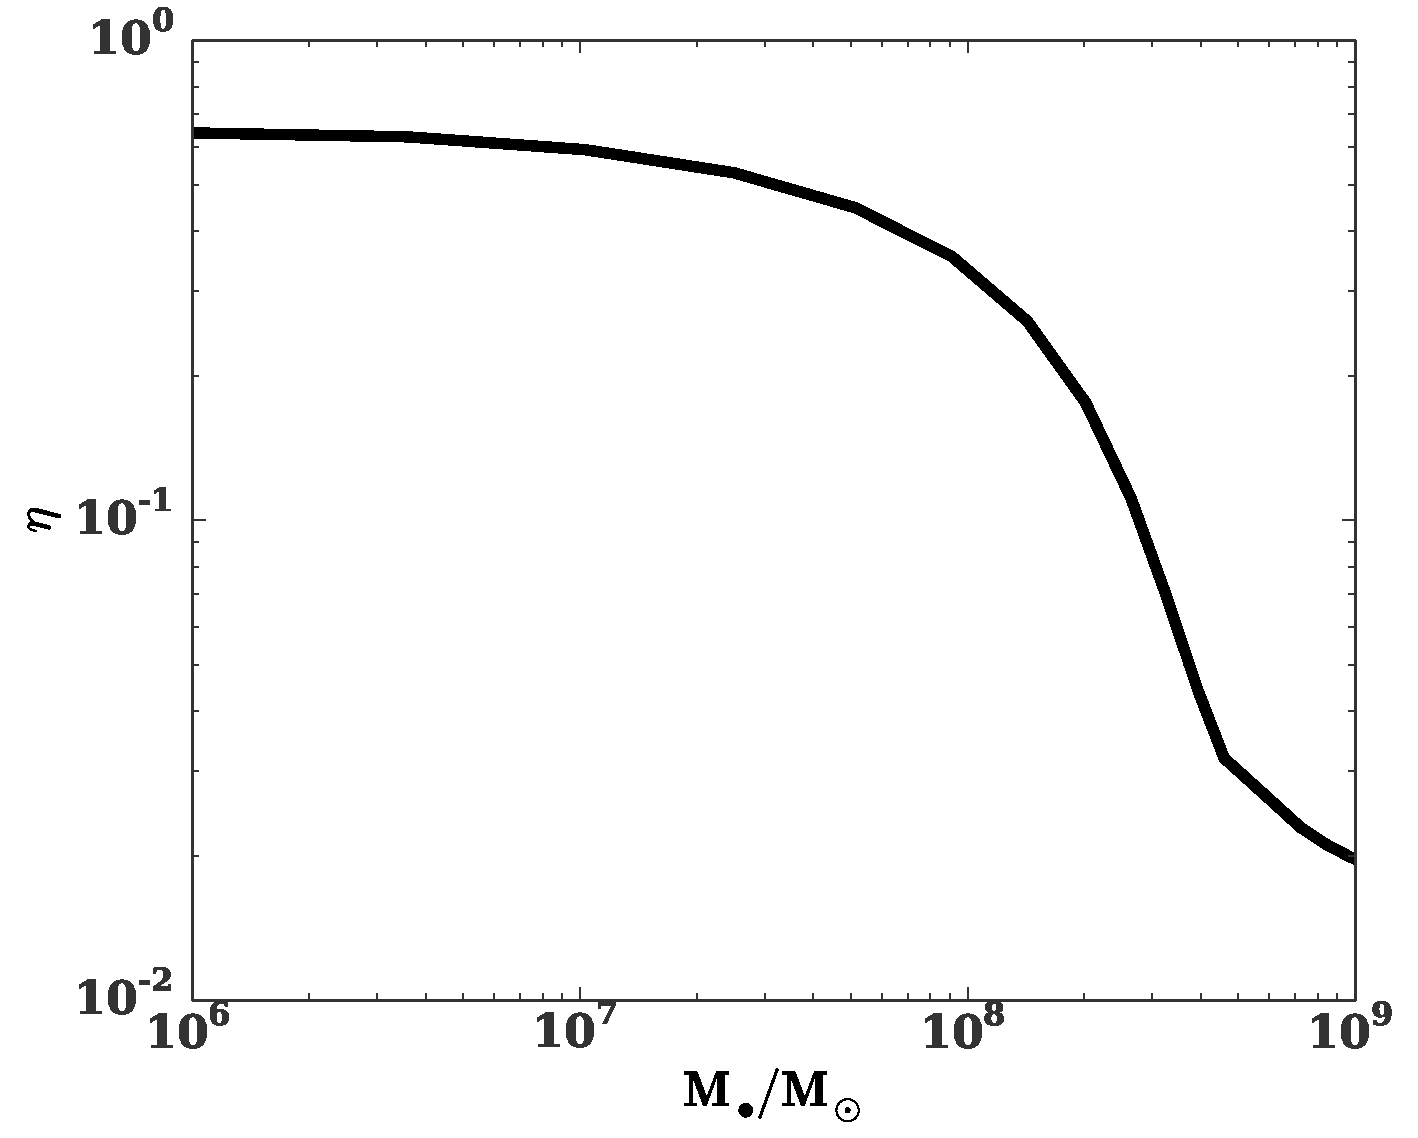
\includegraphics[width=\columnwidth]{eta.pdf}
\caption{\label{fig:eta} Parameter  $\eta$ characterizing stellar mass loss rate (eq.~[\ref{eq:q}]) as a function of black hole mass $\Mbh$, calculated for average star formation histories from \citet{MosterNaab+:2013a} for galaxies with halo masses corresponding to $\Mbh$. }
\end{figure}

For each $\Mbh$ we may check whether the solution for corresponding
$\vwO$ and $\eta$ would be thermally stable, using
equation~\eqref{eq:cooling2} {\bf: AG--double check that this is
  equivalent to what I did.}

The combined heating rate from stellar winds and Compton heating is
insufficient to prevent thermal instability for the high $\Mbh$.  This
is shown in Figure~\ref{fig:cooling2}, which shows the heating over
cooling rate at $\rs$ as a function of $\Mbh$. For $\Mbh\gsim 10^8
\Msun$, the cooling rate will exceed the cooling rate at $\rs$ and
and the gas would be thermally unstable.

\begin{figure}
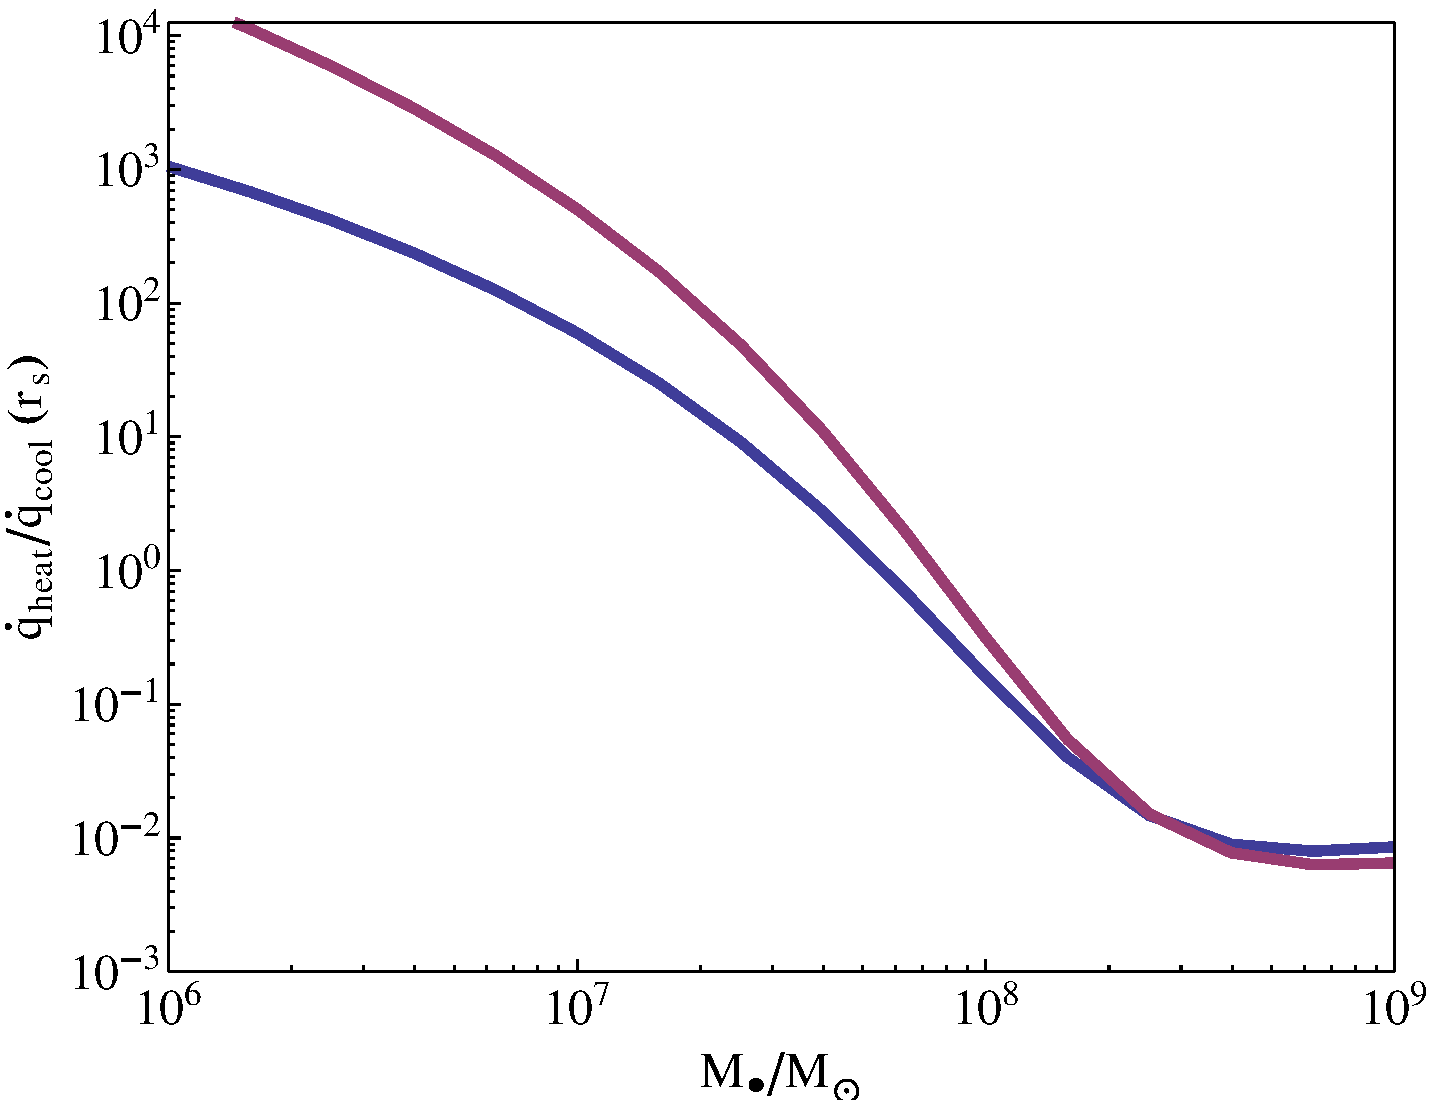
\includegraphics[width=\columnwidth]{cooling2.pdf}
\caption{\label{fig:cooling2} Ratio of heating rate to cooling rate
  $\rs$ versus $\Mbh$ for core ($\Gamma=0.1$) galaxies ({\it dashed})
  and cusp ($\Gamma=0.8$) galaxies ({\it solid}). Ratio is calculated
  using equation~\eqref{eq:cooling2} and the results for $\vwO$ and
  $\eta$ in Figures~\ref{fig:vwSources} and~\ref{fig:eta}}
\end{figure}

Although, in principle the Ia contribution to the heating is
substantial, in practice Ia's occur too infrequently to be a steady
contribution to the heating rate on small scales (e.g. $r_{\rm Ia} >
r_{\rm s}$ as shown in Figure~\ref{fig:rs_rIa}). Thus, SNe Ia heating
by itself would not be able to prevent cooling instability.

\begin{figure}
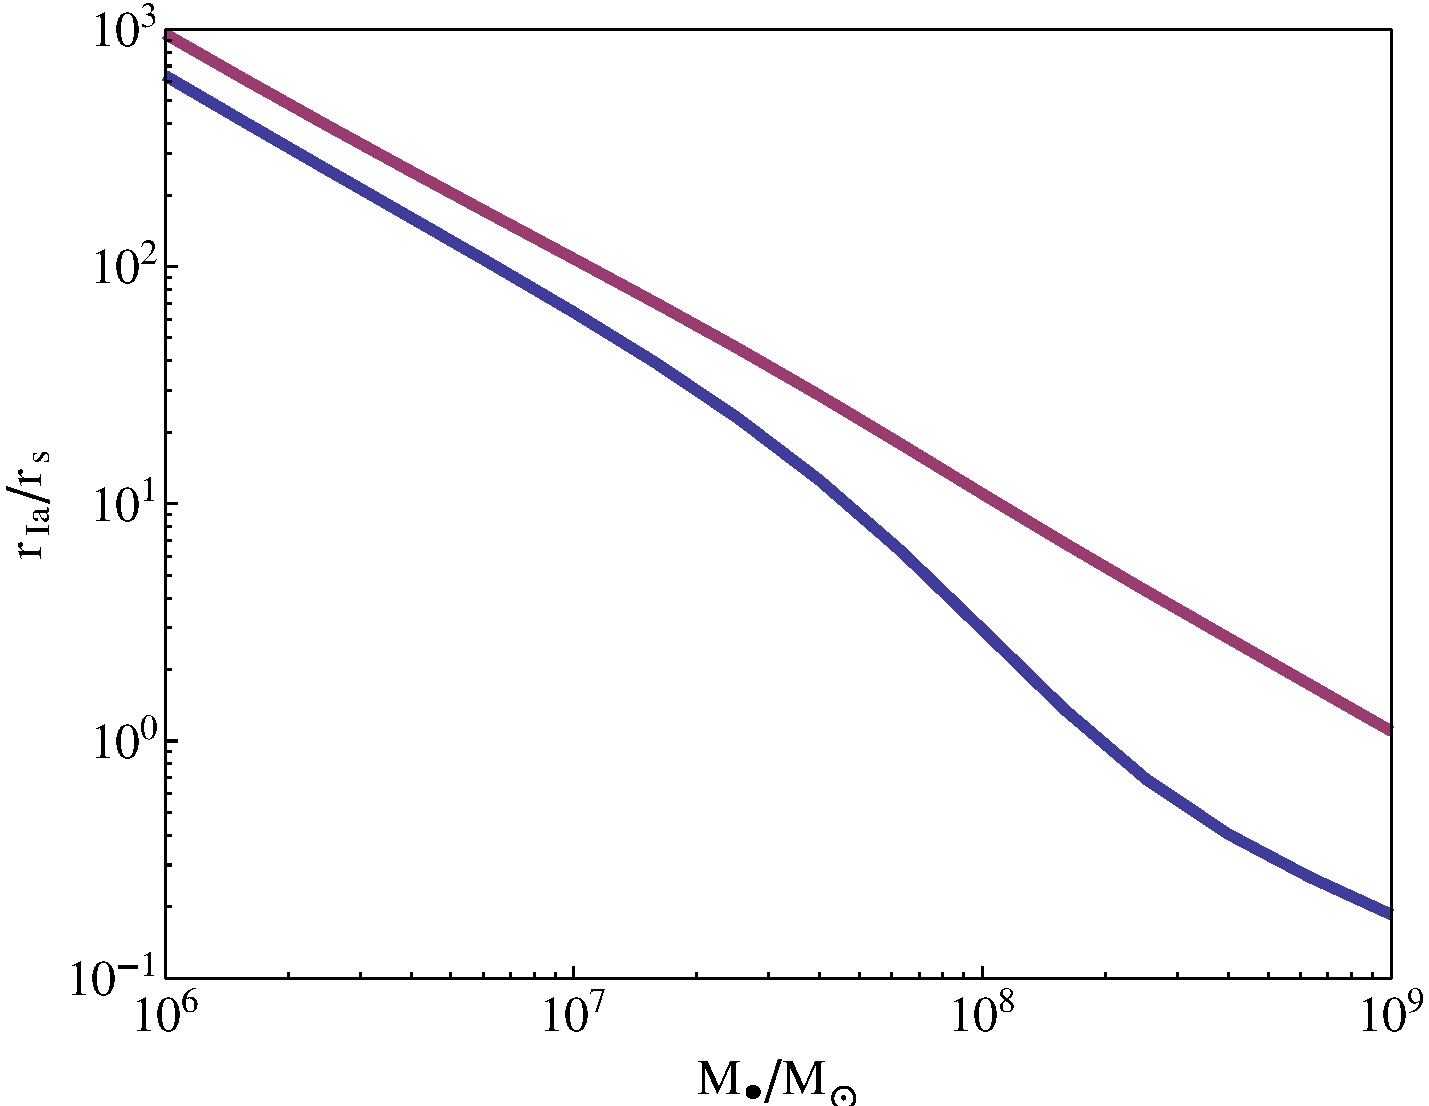
\includegraphics[width=\columnwidth]{rs_rIa.pdf}
\caption{\label{fig:rs_rIa} $\rIa/\rs$ vs. $\Mbh$. $\rIa$ is
  calculated using equation~\eqref{eq:rIa} {\bf AG: I am just
    referring to the first part of the equation here--I use the
    appropriate convolution the Ia rate here}. $\rs$ is calculated
  using the equation~\eqref{eq:stag_simple} and the $\vwO$
  corresponding to each $\Mbh$--see Figure~\ref{fig:vwSources}. For
  the blue curve we use the total $\vwO$ from stars, MSP, and
  black hole feedback (e.g. the solid black curve in
  Figure~\ref{fig:vwSources}). For the purple curve we also include
  the $\vwO$ from Ia's (the dashed red curve
  Figure~\ref{fig:vwSources}).}
\end{figure}

% Figure~\ref{fig:vweff} shows an estimate of how the combined heating
% depends on the age of the stellar population $\tage$ and the SMB mass
% $\Mbh$.  For $M_{\bullet} \gtrsim 1.5\times 10^8 (\tau_{\star}/t_{\rm
%   h})^{0.5} \Msun$, SNe Ia occur sufficiently frequently within the
% stagnation radius (i.e., $r_{\rm Ia} > r_{\rm s}$; eq.~[\ref{eq:rIa}])
% to contribute their full heating rate.  $v_{w}^{\rm Ia} \sim
% 250$ km s$^{-1}$.  On the other hand, for lower mass BHs Ia SNe are
% infrequent, in which case main sequence stars ($v_{w}^{\star}
% \simeq 100-150$ km s$^{-1}$) dominate the heating at most times of
% interest.\footnote{Although SN Ia will still occur surrounding low
%   mass SMBHs, if they are infrequent interior to the radius where the
%   accretion rate is being set, then they will not affect the flow near
%   the SMBH at most epochs.}  For very young stellar populations
% ($\tage \lsim 10^7$ years), $\vwO\simeq 1000$ km s$^{-1}$ due to
% contributions from line driven winds from high mass main sequence
% stars.
{\bf AG: We should mention that regime with stellar wind heating only
  is likely to be thermally unstable.}

 %  \begin{figure}
%     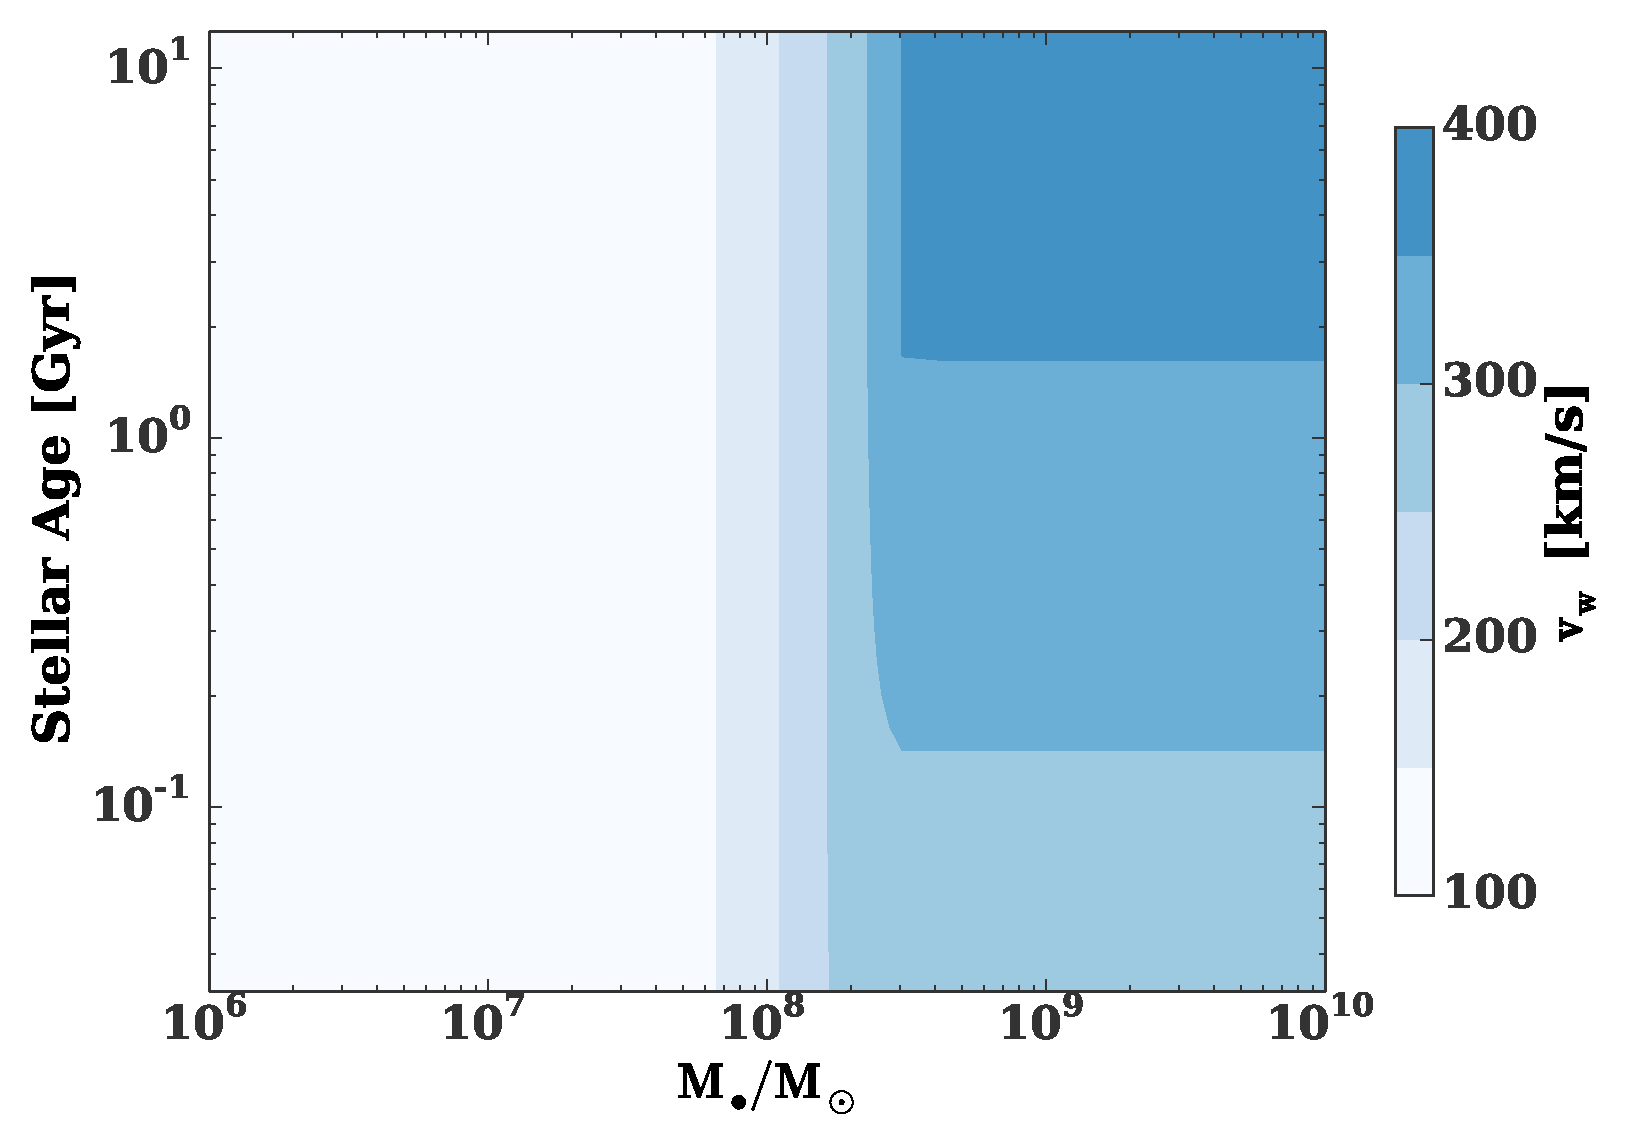
\includegraphics[width=\columnwidth]{vw-contour.eps}
%     \caption{\label{fig:vweff} Combined heating rate $\vwO$ of the CNM
% in the parameter space of SMBH mass $\Mbh$ and age of the stellar
% population $t_{\star}$.  We assume that stellar winds contribute a
% constant heating rate $100$ km/s. The contribution from SNe Ia is
% calculated using equation (\ref{eq:vw_sne}), with thermalization
% efficiency $\epsilon_{\rm Ia}=0.4$. The contribution from SNe Ia is
% only added if the $r_s$ corresponding to the resulting $\vwO$ is
% outside $\rIa$.  {\bf BDM: Correct for dependence of Ia heating on
% time!  among other things}}%describe other cases here.
%   \end{figure}


\section{Applications}
\label{sec:applications}

\subsection{Mass accretion rate}
\label{sec:mdot}

For each solution we calculate the accretion rate $\dot{M}$ onto the
SMBH in units of the Eddington accretion rate $\dot{M}_{\rm edd}
\equiv L_{\rm edd}/0.1 c^{2}$, where $L_{\rm edd} \approx 1.4\times
10^{46}M_{\bullet,8}$ erg s$^{-1}$.  Figure~\ref{fig:mdot_mass} shows
$\dot{M}/\dot{M}_{\rm edd}$ as a function of $\Mbh$ for different
values of $\vwO =$ 300, 600 and 1200 km s$^{-1}$, and for both core
($\Gamma$=0.1) and cusp galaxies ($\Gamma$=0.8).

For fixed wind heating $\dot{M}/\dot{M}_{\rm edd}$ tends to increase
with SMBH mass $\propto M_{\bullet}^{0.5(0.8)}$ for core(cusp)
galaxies, respectively.  This appears to be in contradiction with the
general down sizing trend observed for SMBH accretion in the local
universe (e.g.~\citealt{Heckman+04}; \citealt{Gallo+08}), such as the
fact that for quiescent galaxies the nuclear X-ray luminosity obeys
$L_X \sim \Mbh^\alpha$, where $\alpha\simeq 0.7-0.8$
\citep{MillerGallo+:2014a}.  Our model instead predicts that $\Mdot
\sim \Mbh^{1.5-2}$, such that if $L_x\sim M$, then we would have $\L_x
\sim \Mbh^{1.5-2}$, steeper than the observed relationship.

Hower, the mass accretion rate is also a sensitive function of the assumed heating rate, such that $\dot{M}\sim\vwO^{-3.8(-2.4)}$ for a core(cusp) galaxies, respectively.  Thus, only a weak positive dependence of $v_{w} \propto M_{\bullet}^{0.25-0.3}$ would be sufficient to explain the trend in X-ray luminosity with BH masses in scenarios where $L_X \propto \dot{M}$, or a somewhat steeper dependence $v_{w} \propto M_{\bullet}^{0.35-0.45}$ if $L_{X} \propto \dot{M}^{2}$.  What could cause this dependence?  Maybe Ia SNa...

% This is shown in the top panel Figure~\ref{fig:bh_xray}. The
% relationship from \citealt{MillerGallo+:2014a} and their detection
% upper limits are the black and blue solid lines
% respectively. The points correspond to the $\dot{M} c^2$ for our
% solutions (scaled by $5\times 10^{-7}$).  We must choose a $\vwO$ for
% each galaxy.  We select $\vwO$=200 km/s, roughly the expected level of
% heating expected from main sequence the stellar winds and MSPs. If
% $L_x \sim \Mdot^2$ the discrepancy becomes worse, as shown in the
% bottom panel of Fig.~\ref{fig:bh_xray}, where we plot $2 \times
% 10^{-4} (\eddr) \Mdot c^2$ from our solutions with the relation from
% \citealt{MillerGallo+:2014a}.


One possible solution that the wind mass loss rate $\eta$ increases
with $\Mbh$, as would be expected if low mass SMBH preferentially
hosted younger stellar populations.  Another possible explanation is
that the effective heating rate of the CNM $v_{w}$ decreases
with decreasing SMBH mass.  This could again be due to an older
stellar population, since $v_{w} \propto \eta^{-1/2}$ for heating
sources such as SN Ia and millisecond pulsars.
{\bf AG given our new results on stellar wind heating as a function of
Mbh. It seems like the first statement is indeed true but I suspect
vwO actually increases for low Mbh and that this effect actually dominates.}
%, or it could be due to the fact that Ia occur too infrequently inside
%the stagnation radius for low mass black holes.
%AG-We now think that SNe Ia would become important only at the
%highest values of Mbh.
%AG-Note sure where the best place for this discussion would
%be--here or after presenting the comparisons with Miller et al.

\begin{figure}
  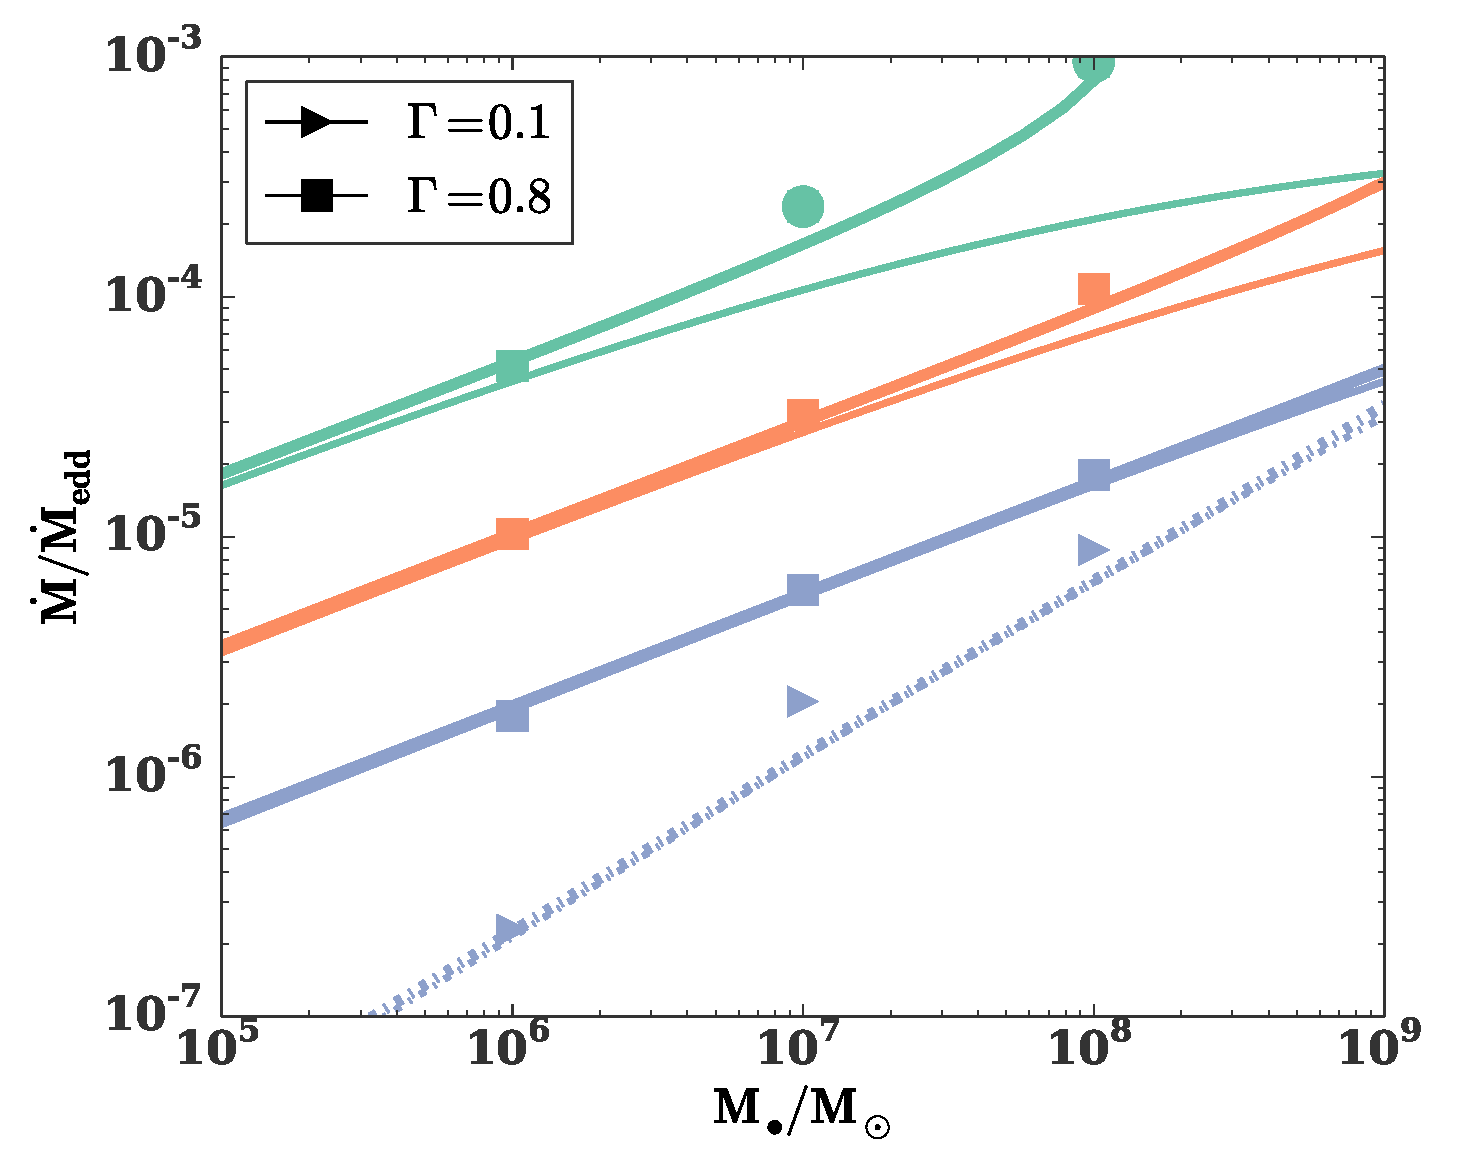
\includegraphics[width=\columnwidth]{mdot_mass.eps}
  \caption{\label{fig:mdot_mass} Accretion rate $\dot{M}$ in units of
    the Eddington rate $\dot{M}_{\rm edd}$ as a function of SMBH mass
    for each galaxy in our sample, calculated for different values of
    the wind heating parameter $\vwO =$ 300 km s$^{-1}$ ({\it green}),
    600 km s$^{-1}$ ({\it orange}), and 1200 km s$^{-1}$ ({\it blue}).
    Squares correspond to cusp galaxies ($\Gamma=0.8$), while
    triangles correspond to cores ($\Gamma$=0.1). The curves correspond
    to the analytic results for $\eddr$ from equation
    (\ref{eq:eddr_analytic}) for cusps (solid lines) and cores (dashed
    lines).  }
\end{figure}

%% AG:  Also want to include a plot of x-ray luminosity (less abstract than the accretion rate). 

\subsection{Comparison to Observations}
{\bf AG: I do want some discussion of reproducing the density profiles
for individual observations, but I am not sure how to do it with our
new gridded approach.}
% \subsubsection{Comparison to measured temperature and density profiles}
% \citet{AllenDunn+:2006a} use {\it Chandra} X-ray observations to infer the radial temperature and density profiles in the nuclei of nine nearby X-ray luminous elliptical galaxies.  \citet{RussellMcNamara+:2013a} performed a similar analysis with a somewhat enlarged galaxy sample.  Interestingly, these works find a correlation between the accretion rate inferred assuming Bondi accretion and the AGN jet power, which is estimated by the PdV work required to inflate observed cavities in the X-ray emitting gas.  
% % At some point it would be useful to describe the differences between
% % these two sets of observations \citealt{RussellMcNamara+:2013a}
% % tries several different extrapolation schemes for the gas density,
% % and finds that that the uncertainty in extrapolating the density
% % profile is the dominant source of uncertainty in measuring the
% % accretion rate. Find total number which overlaps once the Russell
% % galaxies are included...

% Five of the galaxies in the \citet{AllenDunn+:2006a} sample overlap with that in \citetalias{WangMerritt:2004a}.  We may thus compare our results for the $T$ and $\rho$ profiles with those inferred from observations for the overlapping galaxies.  The results of this exercise are presented in Fig.~\ref{fig:allen_compare}.

% Note that we have two free parameters ($\eta$ and $\vwO$) in our
% model, which implies that we can always match the observed temperature
% and densities at at least one point.  As a general rule, we find that
% a wind heating parameter $\vwO=500$ km s$^{-1}$ gives rough agreement
% with the observed temperatures.  We now highlight results for specific
% galaxies.
% % Thus, we choose $\vwO=500$ km/s.  We choose an
% % $\eta$ so that our solution would be consistent with the observed
% % density profiles. The comparison is shown in
% %% AG-The chosen properties, in particular eta may be summarized in a tabe.
% %% AG-Mention rising temperature profiles on large scales.

% \begin{itemize}
% % \item \emph{NGC4486} %eta=0.2
% %   On scales of $\sim1$ kpc the density profile in
% %   \citealt{AllenDunn+:2006a} is shallower than in our model. Our model
% %   has a break in the gas density at $\sim 300$ pc--near the location
% %   of the Nuker break radius for this galaxy at 560 pc. There is an
% %   observed break in the density, but on a scale of a few kpc.

% %   The temperature is assumed to be flat from the resolution limit
% %   inwards in \citealt{AllenDunn+:2006a}. However, in our models $T$
% %   increases monotonically towards the galactic center. This increase
% %   is due to the increased velocity dispersion (and thus increased
% %   heating) towards the galactic center.

% \item \emph{NGC5813} %eta=0.1 
%   The observed density profile (\citealt{RussellMcNamara+:2013a}) is
%   shallower than our calculated density profile, which has a sharp
%   break at $\sim$0.1 kpc, the location of the break radius in the
%   Nuker profile (this is the radius where the stellar light profile
%   transitions from a shallower inner power law slope to a steeper
%   outer power law slope).

%   For this galaxy we found that we could reproduce the observed
%   temperature on large scales with $\vwO=500$ km/s. The increased
%   velocity disperision towards the galactic center results in a sharp
%   increase in $T$ at small radii, which is not captured in the
%   observations due to resolution issues.
% \end{itemize}

% %It would be nice to have error bars for the observational points in this plot...
% \begin{figure*}
%   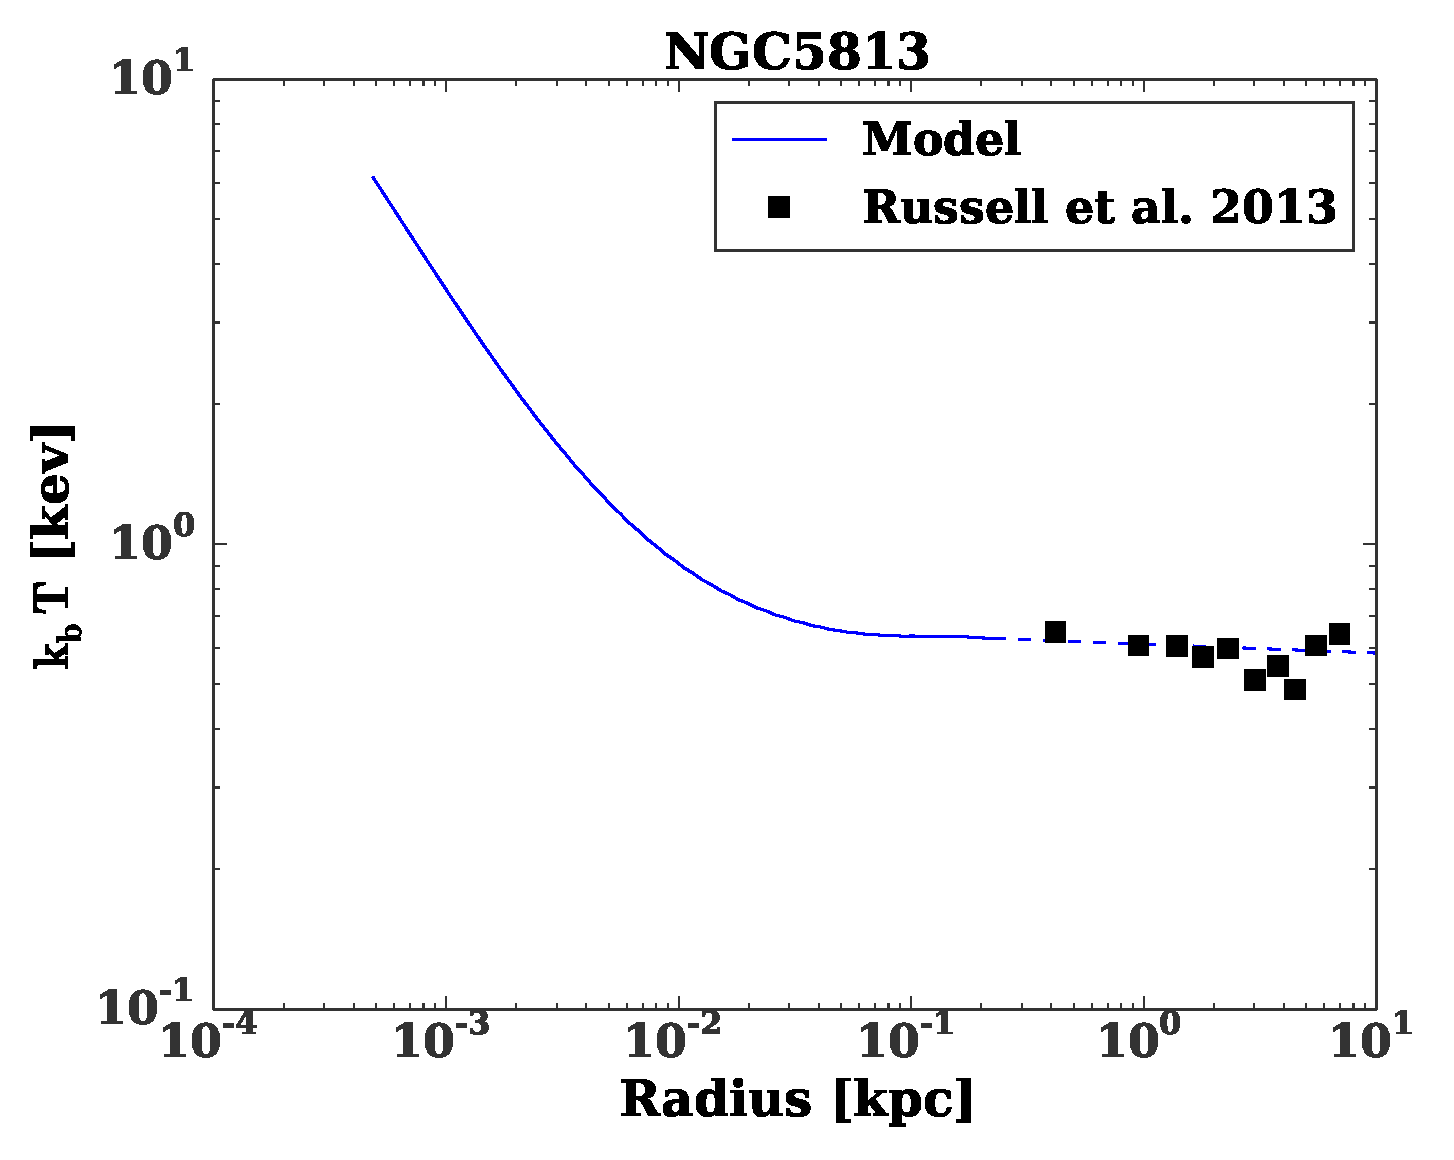
\includegraphics[width=\columnwidth]{NGC5813_T.eps}
%   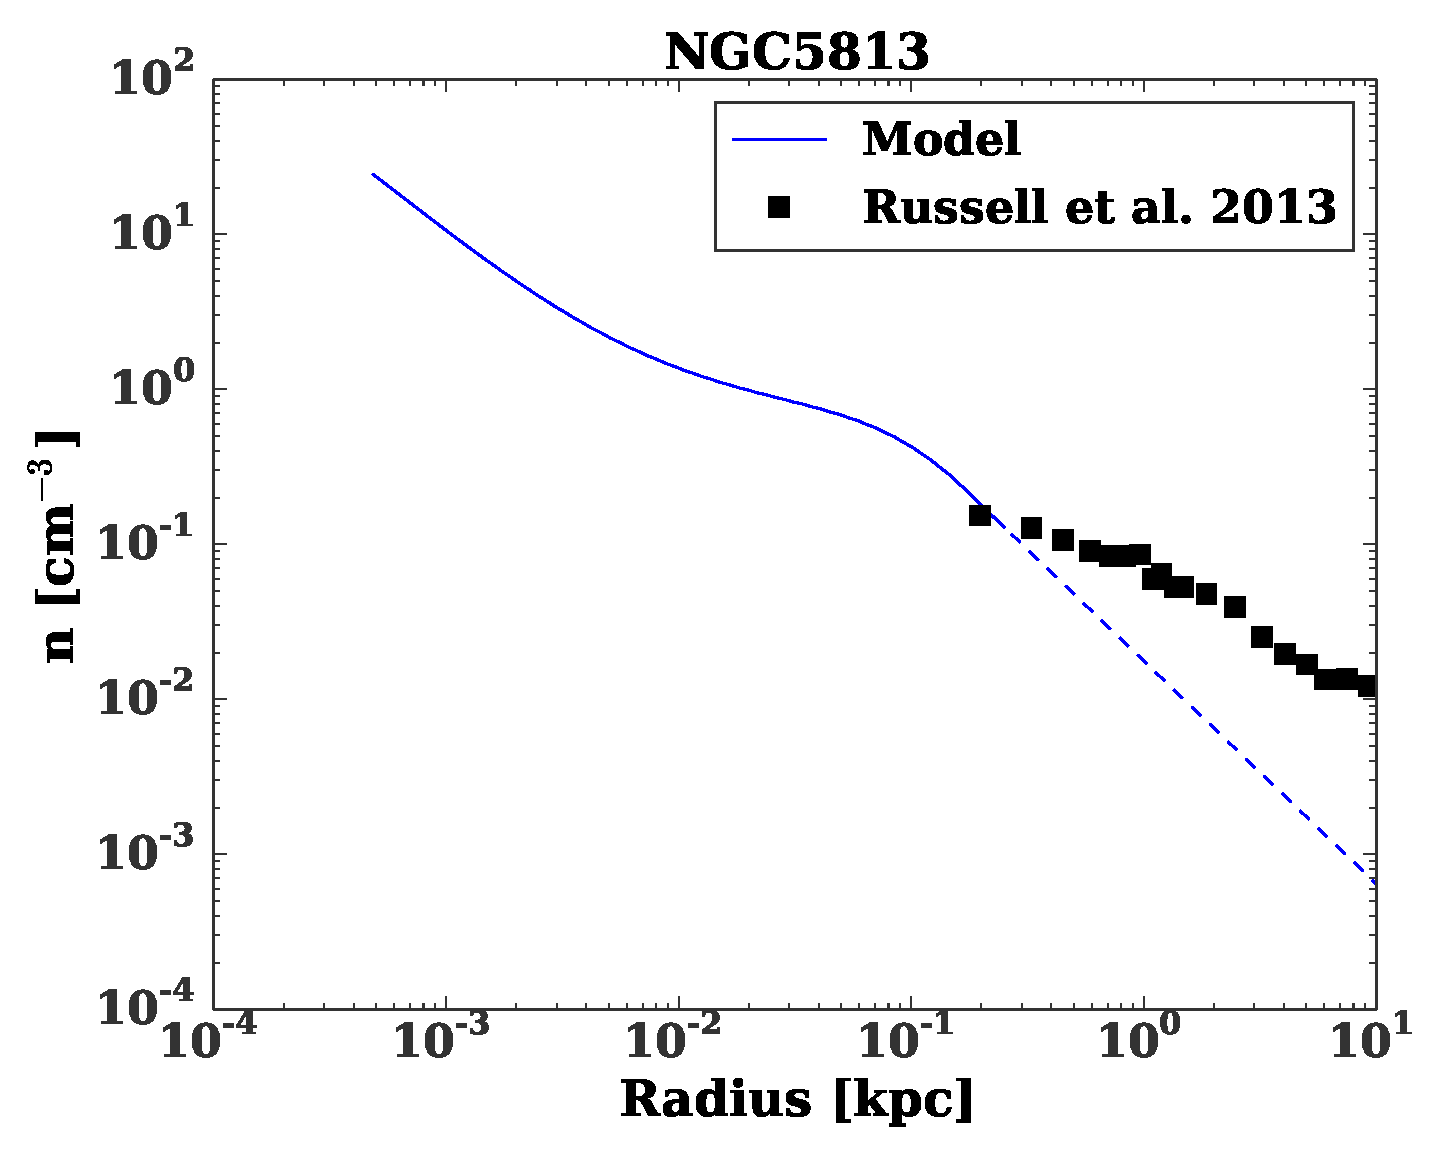
\includegraphics[width=\columnwidth]{NGC5813_rho.eps}
%   \caption{\label{fig:allen_compare} Comparison of the radial profiles
%     (blue lines) of electron number density $n_e$ and temperature $T$
%     to the measured values (black square) in \citet{AllenDunn+:2006a}
%     and \citet{ RussellMcNamara+:2013a}. The dashed blue lines are
%     power law extrapolations of our profiles. Note that in going from
%     $\rho$ to $n_e$ we our adopted value for the molecular weight $\mu=1$.}
%   %% AG in the future we will have to be carfeful of the mean molecular weight.
% \end{figure*}

% \subsubsection{Comparison with observed X-ray Luminosity-Mass
%   Relation}
% %Note currently I reverse-engineer the stellar mass from the black
% %hole mass inferred from M-sigma; however, it would be better to use
% %the tabulated black hole mass from the Mbh-Mbulge relation.
% Fig. 1 of \citealt{MillerGallo+:2014a} plots the observed
% relationship of unresolved x-ray luminosity versus galactic stellar
% mass for a sample of quiescent galaxies. We may construct a similar
% relationship with our own sample using the inferred accretion rates
% from our solutions.  To infer an x-ray luminosity for each solution,
% we scale our calculated $\Mdot c^2$ by a constant. We pick $5\times
% 10^{-7}$, which gives x-ray luminosities comparable to
% those in \citealt{MillerGallo+:2014a}. We also try an alternate
% prescription in which $L_x$ is quadratic in $\Mdot$. In particular, we
% take $L_x=2 \times 10^{-4} (\eddr) \Mdot c^2$. 

% We must make choose a $\vwO$ for each galaxy.  We select $\vwO$=200
% km/s if $\rs<\rIa$ for this solution, $\vwO$=500 km/s if $\rs>\rIa$
% for this solution, or exclude it.  At low $\Mbh$ we have $\vwO$=200
% km/s and at high $\Mbh$ we have $\vwO$=500 km/s.  Note that much of
% our sample is excluded in this Fig., since for $\vwO$=200 km/s we
% would have $\rs>\rIa$ and four $\vwO$=500 km/s we would have
% $\rs<\rIa$ (i.e. the relative locations of $\rs$ and $\rIa$ would be
% inconsistent with the assumed level of heating).

% %AG-power law may be closer to 1.4 & 1.8 than to 1.5 & 2.
% Our results are plotted in Fig.~\ref{fig:bh_xray}. In our model
% there is a steeper dependence $\Mbh$ on $M_{\rm gal}$ than in
% \citealt{MillerGallo+:2014a}. We find $L_x \propto M_{\rm gal}^{1.5}$ when
% $L_x \propto M_{\rm gal}^{2}$, whereas \citealt{MillerGallo+:2014a} finds
% that $L_x \propto M_{\rm gal}^{0.7-0.8}$. 

% \begin{figure}
% 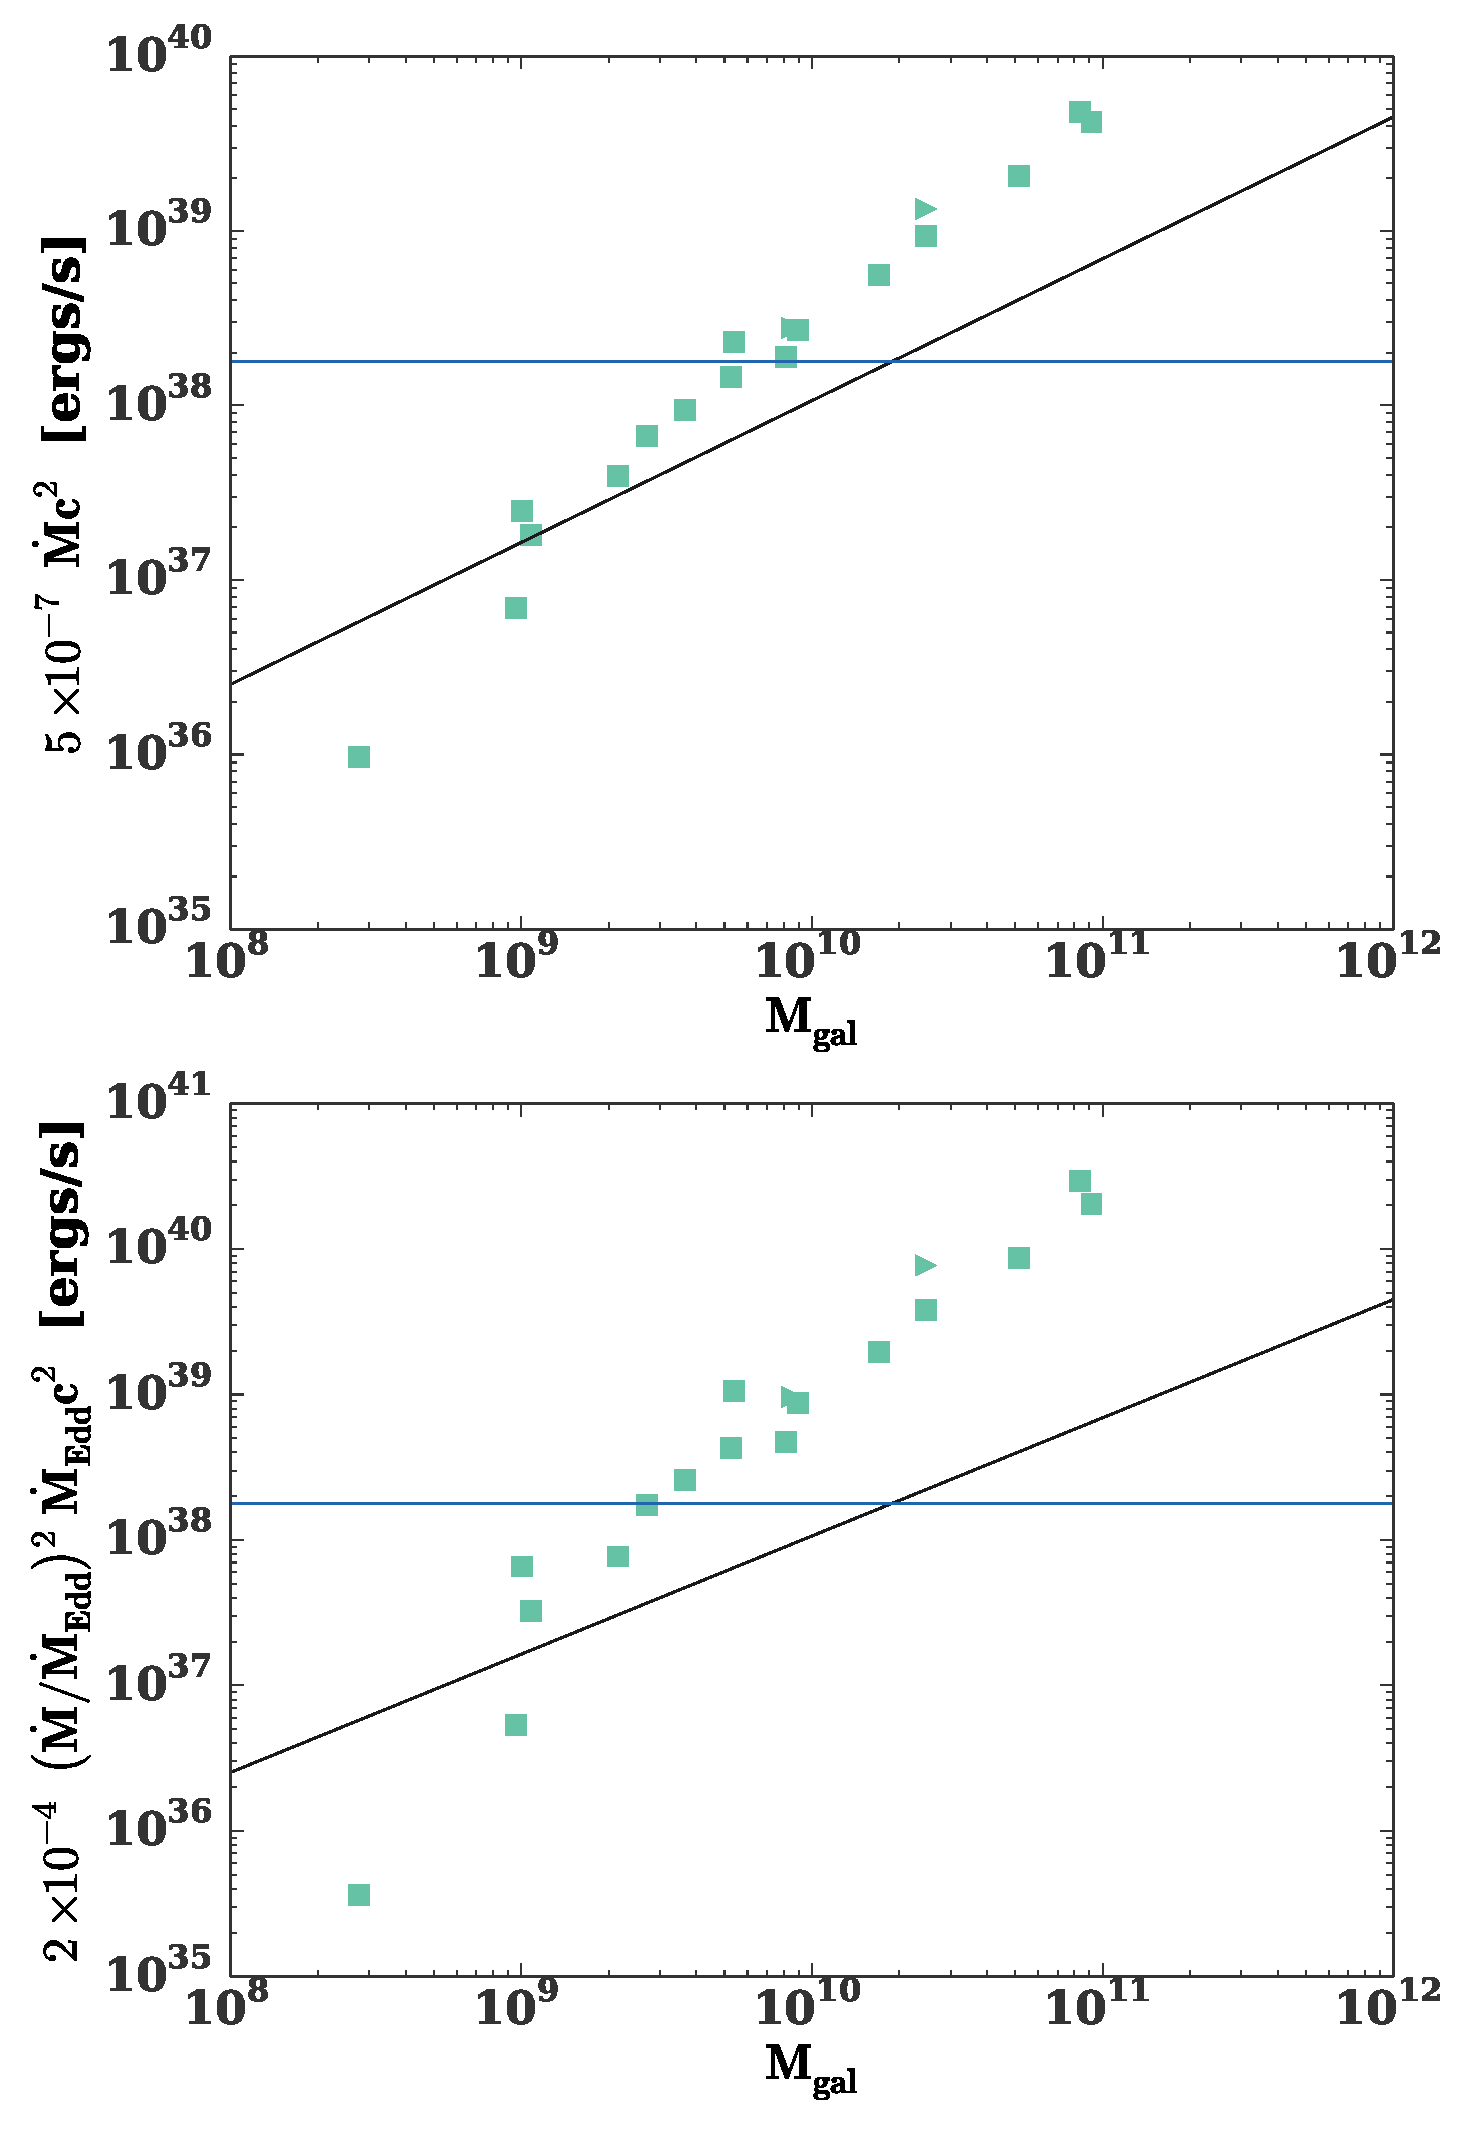
\includegraphics[width=\columnwidth]{bh_xray.eps}
% \caption{\label{fig:bh_xray} X-ray luminosity plotted as a function of
%   stellar mass for our solutions (points), the trend of nuclear x-ray
%   luminosity with stellar mass (black line) and the detection upper
%   limit (blue line) from Fig. 1 of \citealt{MillerGallo+:2014a}. In
%   the top panel we take the X-ray luminosity to be $\epsilon_1 \Mdot
%   c^2$, with $\epsilon_1=5\times 10^{-7}$ chosen to make our
%   luminosities comparable to those observed. In the bottom panel, we
%   take the accretion power to be quadratic in $\Mdot$. $L_x=\epsilon_2
%   \eddr \Mdot c^2$ with $\epsilon2$=$2\times10^{-4}$. For each galaxy
%   we choose the $\vwO=200$ km/s solution.  {\bf BDM: if possible, add actual x-ray data from Gallo+08!}}
% \end{figure}

\section{Discussion}
\label{sec:discussion}

\subsection{Demographics of SMBHs}

Our analytic expression for the accretion rate (eq.~[\ref{eq:mdot_analytic}]) can be translated into the growth time of the SMBH $t_{\rm grow} \equiv M_{\bullet}/\dot{M}$,
\begin{eqnarray}
  t_{\rm growth}/t_{\rm h} \approx 
  \begin{cases}
    250 M_{\bullet,8}^{-0.76}
    v_{500}^{3.8}   \eta_{0.02}  & \text{core} \\
    140 \Mbheight^{-0.48}
    v_{500}^{2.4}   \eta_{0.02}  & \text{cusp}, 
  \end{cases}
  \label{eq:tgrow_analytic}
\end{eqnarray}
which we have normalized in terms of the Hubble time.  

{\bf BDM: ADD plot of parameter space of MBH and stellar age, showing Ia heating versus stellar heating; thermally stable versus unstable regions ($t_{\rm ff} = t_{\rm cool}/10$); as well as where $\sigma = v_{w}^{\bullet}$ and $\sigma = v_{w}^{\star}$.  }

\subsection{Cooling}
\label{sec:cooling}

  \subsection{Angular Momentum}
  \label{sec:ang}
  Our models are spherically symmetric and do not include the effects of
  the gas' angular momentum. However, galaxies will in general have some
  net rotation, and the gas will generally have some non-zero angular
  momentum. At some radius, $\rcirc$, the specific angular momentum of
  the gas will equal the specific angular momentum of a circular
  orbit. Inside of this radius our assumptions of no rotation and
  spherical symmetry will break down. But if $\rcirc$ is inside of the
  inner sonic point of the flow, the region where angular momentum
  becomes important will be causally disconnected from the rest of the
  flow, and we would be justified in neglecting angular momentum (at
  least on large scales).

  $\rcirc$ depends on the gas injection radius. The largest
  injection radius is $\rs$. Let $\lrs$ be the gas specific angular
  momentum at $\rs$, then 

  \begin{align}
    \rcirc=\frac{\lrs}{G \Mbh}
  \end{align}

  \citet{EmsellemCappellari+:2007a} used two-dimensional kinematic
  data to measure the ratio of ordered to random motion in a sample of
  early type galaxies. More precisely, they measure

  \begin{align}
    \lambda_R=\frac{\left<R|V|\right>}{\left<R\sqrt{V^2+\sigma^2}\right>}
  \end{align}

  Where $R$ is the distance is the distance from the galactic center, $V$ is
  the mean stellar velocity, and $\sigma$ is the velocity
  dispersion. The brackets represent a luminosity weighted average.

  We may rewrite the specific angular momentum at $\rs$ in terms of
  $\lambda_R$.

  \begin{align}
    \lrs\simeq\lambdars \sigma|_{r_{\rm s}}^2 \rs^2
  \end{align}

  Then

  \begin{align}
    \rcirc&\simeq\lambdars^2 \frac{\sigma|_{r_{\rm s}}^2}{G \Mbh} \rs^2\\
    &\simeq\lambdars^2 \frac{\rs^2}{\rsoi} \lsim \lambdars^2 \rsoi
  \end{align}

  The inner sonic point, $\rss$ general occurs at $\simeq 1\%$ of
  $\rsoi$. {\bf AG need to explain this somehow. Also, note in our
    simulations the inner sonic point is not properly resolved.}
  So if $\lambdars\lsim 0.1$, $\rcirc<\rss$. In Fig. 2 of
  \citet{EmsellemCappellari+:2007a} $\lambda_R$ is plotted as function
  of radius for a sample of early type galaxies. On scales of $\sim 0.1
  R_e$ $\lambda_R$ is either less than 0.1 or rapidly declining for most
  of their sample %%need to be clearer on rapidly declining also compare
  %% this scale to the sphere of influence scale.
  This suggests that angular momentum should generally be unimportant.

\section{Discussion}

\begin{itemize}
\item{Fact that some low mass BHs appear to have nearly Eddington accretion rates, suggest an external origin - since the maximum Ia rate appears to be below this}
\end{itemize}

If cooling becomes important in the flow ($\tilde{v}_{w} < v_{\rm CI}$), it may lead to thermal instabilities.  There are two kinds of ``instabilities", global and local.  The global instability is simply that, if cooling becomes very rapid, the gas loses thermal pressure and starts to inflow faster, i.e. the entire CNM accretes.  In
practice this should could manifest as a large increase in the stagnation radius, due an effective {\it decrease} in the effective heating rate.  This global ``instability" is not a true instability insofar as the gas does not necessarily clump locally into low-T clouds.

However, \citet{McCourt+12} argue that even if cooling is exactly
balanced by heating everywhere, there is still a local thermal
instability that operates to turn hot gas into cold clouds.  However,
this local instability only causes a significant local drop-out of
mass from the hot medium (to low-T clouds), if the cooling timescale,
\begin{align}
\frac{\tcool}{\tff} &\equiv \frac{3\rho k T/2 \mu \mp}{\dot{q}_{\rm cool}} \approx \frac{9}{5} \left. \frac{q \vw^2/2}{\dot{q}_{\rm cool}}\right|_{\rs}
\end{align} 
is locally shorter than the approximately 10 times the free-fall
timescale $t_{\rm ff}$, where the last equality is evaluated at the
stagnation radius and makes use of equations~(\ref{eq:Tanalytic}) and
(\ref{eq:rhors2}).  We thus see that the condition $\tilde{v}_{w} \gtrsim v_{\rm
  crit}$ is also the condition for local instability, although the
prefactor may be slightly different.

\subsection{TDE Jets}

Plot showing final lorentz factor after the reverse shock crossing as a function of BH mass, using average star formation history.  place J1644+57 on the plot.

\subsection{Jet Power Correlation}

Accretion rates onto SMBHs can in principle be estimated directly by
assuming Bondi accretion and using high resolution X-ray observations
to estimate the gas temperature and density near the Bondi radius.
This technique has led to the intriguing conclusion that the Bondi
accretion power correlates with the AGN jet power (e.g.,
\citealt{AllenDunn+:2006a}; \citealt{Russell+13};
\citealt{FujitaKawakatu+:2014a}), the latter estimated from the energy
required to inflate the observed cavities within the X-ray emitting
gas.  In practice is it almost never possible to resolve the Bondi
radius, therefore requiring all such studies to extrapolate the
observed gas temperature and density profiles to smaller radial
scales.

\subsection{Nuclear Star Clusters}
Do nuclear star clusters in other galaxies look like scaled up/down
versions of the one in our own galaxy? If so this would imply a radial
gradient in the average of the stellar population which would imply a
heating which would be dependent on radius.

\subsection{SFR-AGN connection}
In fact it seems like the star formation rate may trace AGN
episodes. See e.g. http://arxiv.org/pdf/1501.07602.pdf. 

\subsection{Type II Supernovae}
Type II supernovae should provide some heating as well for younger
stellar populations...In fact at least on large scales they may be the
dominant source of heating on timescales of 10-40 Myr. 
  

  \section{Summary}
  \label{sec:summary}
  We have calculated steady-state models for circumnuclear medium of a
  sample of early type galaxies, assuming that gas is supplied
  entirely by stellar wind mass loss and heated by shocked stellar
  winds and SNe Ia. We may use these profiles to calculate an $\Mdot$
  onto each of sample galaxy's SMBH, and get the scaling of $\Mdot$
  with $\Mbh$. We may then compare our results with observed trends of
  nuclear x-ray luminosity. Our main conclusions may be summarized as
  follows.

  \begin{enumerate}
  %Younger population=>higher accretion rate; generally higher eta and
  %lower vw except for very young stellar populations.
  \item We find that $\eddr \propto \Mbh^{\alpha}$, where the value of
    $\alpha$ depends on the slope of the stellar density profile
    ($\alpha\simeq0.5,1$ for cusp and core galaxies respectively). One
    possible solution that the wind mass loss rate (i.e. $\eta$)
    increases with $\Mbh$, as would be expected if low mass SMBH
    preferentially hosted younger stellar populations. Another possible
    explanation is that the effective heating rate of the CNM $v_{w}$
    decreases with decreasing SMBH mass. This could again be due to an
    older stellar population, since $v_{w} \propto \eta^{−1/2}$
    for heating sources such as SN Ia and millisecond pulsars.
  \item We compare the $\Mdot$ for each of our solution to the one
    calculated from the Bondi formula. We find that they generally to
    a factor of a few. In our model the accretion rate is determined
    from the gas properties at the stagnation radius, $\rs$, which
    agrees with the Bondi radius, $\rb$, within a factor of a
    few. Thus, use of the Bondi formula is a good approximation.
  \item We compare our solutions for density and temperature to those
    inferred from Chandra x-ray observations by \citet{AllenDunn+:2006a}
    and \citet{RussellMcNamara+:2013a} for a handful of galaxies in
    which our sample overlap with theirs. In general, we cannot match
    the observed gas density slope on large scales. 
  \end{enumerate}
  
  \clearpage
  \appendix
  \section{Analytic Expression for the stagnation radius}
  \label{app:rs}
  
Here we derive an analytic expression for the steady-state stagnation radius $r_{\rm s}$.  The steady-state entropy equation (eq.~[\ref{eq:dsdt}]) can be manipulated to read
\begin{align}
T\dsdr=\frac{\Q}{\rho v} \label{eq:ss_entropy}
\end{align}
By definition, the velocity $v$ goes to zero at the stagnation radius.  In order to avoid the entropy derivate from diverging, the numerator of (\ref{eq:ss_entropy}) must also go to zero at $r_{\rm s}$, implying that
\begin{align}
 \frac{\gamma}{\gamma-1} \frac{p|_{\rs}}{\rho|_{\rs}}=\frac{\vw^{2}|_{\rs}}{2} \Rightarrow \frac{\kb T|_{\rs}}{\mu \mp}=\gammafi \frac{\vw^{2}|_{\rs}}{2} .
\label{eq:appTanalytic}
\end{align}
Combining (\ref{eq:ss_entropy}) with the first law of thermodynamics,
\begin{align}
T\dsdr =& \frac{1}{\gamma-1}\ddr{(p/\rho)}-\frac{p}{\rho^2}\ddr{\rho} = \\
& 
\frac{1}{\gamma-1}\left.\ddr{(p/\rho)}\right|_{\rs}+\frac{\densSlope}{\rs}  \frac{p|_{\rs}}{\rho|_{\rs}}=\left.\underbrace{\frac{\Q}{\rho  v}}_{A}\right|_{\rs}, 
% \label{eq:first_law}
\end{align}
where $\densSlope\equiv -\left.d\log(\rho)/d\log(r)\right|_{\rs}$.  The term on the right can be evaluated using L'Hopital's rule, yielding
%\begin{align}
 % &\lim_{r \rightarrow \rs} A=\frac{\lim_{r \rightarrow \rs}
  %  \frac{d}{dr}\left[q (r)\left(\ke -\gammaf
   %     \frac{p}{\rho}+\kew\right)\right]}{\lim_{r \rightarrow \rs}
    %\frac{d}{dr} \left(\rho v\right)}\\
  %&=\frac{ q'|_{\rs} \overbrace{\left.\left(\ke
   %     -\gammaf\frac{p}{\rho}+\kew\right)\right|_{\rs}}^0+ q|_{\rs}
    %\frac{d}{dr} \left[\left(\ke -\gammaf
     %   \frac{p}{\rho}+\kew\right)\right]_{\rs}}{\underbrace{\rho'|_{\rs}
      %v|_{\rs}}_0 +\underbrace{v'|_{\rs}\rho|_{\rs}}_{q|_{\rs}}}\\
\begin{align}
  \lim_{r \rightarrow \rs} A = \frac{d}{dr} \left[\left(\ke -\gammaf \frac{p}{\rho}+\kew\right)\right]_{\rs}
\end{align}
Now using the definition $\vw^2=\vwO^2+ G \Menc/r$, where
$\Menc=\Mbh+\Mstar$, and assuming $\Mstar \sim r^{2-\Gamma}$, we find that
\begin{align}
\lim_{r \rightarrow \rs} A=-\gammaf
\left.\ddr{(p/\rho)}\right|_{\rs}-\frac{G \Menc|_{\rs}}{2 \rs^2}+(2-\Gamma) \frac{G
  \Mstar|_{\rs}}{2 \rs^2}.
\end{align}
Substituting this expression back into equation (\ref{eq:first_law}) and using equation (\ref{eq:appTanalytic}) gives
\begin{align}
&\frac{\gamma+1}{\gamma-1}
\left.\ddr{(p/\rho)}\right|_{\rs}+ \frac{\gamma-1}{\gamma} \frac{\densSlope}{\rs} \vw|_{\rs}^{2} = (2-\Gamma) \frac{G
  \Mstar|_{\rs}}{2 \rs^2} -\frac{G \Menc|_{\rs}}{2 \rs^2}.  \label{eq:rs1}
\end{align}
A second equation results from evaluating the momentum equation (eq.~[\ref{eq:dvdt}]) at the stagnation point
\begin{align}
&\frac{1}{\rho}\dpdr=- \frac{G\Menc}{\rs^2} \Rightarrow
&\ddr{(p/\rho)}+\frac{p}{\rho}
\underbrace{\frac{d\log(\rho)}{dr}}_{-\densSlope/r} = -\frac{G \Menc}{\rs^2} \label{eq:HSE}
\end{align}
Finally, combining equations (\ref{eq:rs1}) and (\ref{eq:HSE}) gives 

\begin{align}
\rs=\frac{G \Mbh}{\densSlope \vw^{2}|_{\rs}}\left(\frac{9-\Gamma}{2}
  \frac{M_{\star}|_{\rs}}{\Mbh} +\frac{7}{2}\right),
\end{align}
where we have assumed $\gamma=5/3$.

In terms of just the additional wind heating parameter, $v_w$,

\begin{align}
\rs=\frac{G \Mbh}{\densSlope v_w^{2}|_{\rs}}\left[\left(\frac{9-\Gamma}{2} -\densSlope\right) \frac{\Mstar|_{\rs}}{\Mbh} +\frac{7}{2}-\densSlope\right].
\label{eq:rs2main}
\end{align}


Defining $\eta \equiv \vwO/\sigma_{\rm soi}$, this relationship can be
reparameterized as follows:
\begin{align}
  \frac{\rs}{\rsoi}=\frac{1}{2 \zeta^2 \densSlope}\left[
    \frac{\Mstar|_{\rs}}{\Mbh}\left(\frac{9-\Gamma}{2}-\densSlope\right)+\left(\frac{7}{2}-\densSlope\right)\right]
\end{align}

%{\bf AG: Note that I have taken sigmainf=2 G Mbh/rinf. Commented out
%equations have sigmainf=G Mbh/rinf}. 
For cusp galaxies ($\Gamma\simeq1$) we have $\Mstar|_{\rs}/\Mbh=x$, $A=4$, and $B=7/2$ for $\gamma = 5/3$, such that 
\begin{align}
\x=\frac{7-2\densSlope}{4\zeta^2 \densSlope+2\densSlope-8}
%\x=\frac{7-2\densSlope}{2\zeta^2 \densSlope+2\densSlope-8}
\end{align}
In the limit of zero wind heating $\eta \rightarrow 0$, no solution
for $r_{\rm s}$ exists unless the gas density profile at the
stagnation radius is steep, 3.5 $<\densSlope<$ 4.

For core galaxies ($\Gamma \simeq 0$) with $\Mstar/\Mbh=x^2$, A=9/2,
and B=7/2, the stagnation radius instead obeys a quadratic equation
\begin{align}
\x=\frac{\zeta^2 \densSlope \pm \sqrt{\zeta^4 \densSlope^2 - \left(\frac{9}{2}-\densSlope\right)
    \left(\frac{7}{2}-\densSlope\right)}}{\left(\frac{9}{2}-\densSlope\right)}
%\x=\frac{\zeta^2 \densSlope \pm \sqrt{\zeta^4 \densSlope^2 - 4 \left(\frac{9}{2}-\densSlope\right)
%\left(\frac{7}{2}-\densSlope\right)}}{2 \left(\frac{9}{2}-\densSlope\right)}
\label{eq:rstag}
\end{align}
In this case no solution exists in the zero heating limit ($\zeta
\rightarrow 0$) unless $3.5<\densSlope<4.5$.

When $\Mstar << \Mbh$ at the stagnation radius, the relationship
between $\rs$ and $\vw$ is greatly simplified.
\begin{align}
\rs=\frac{7}{2}\frac{G \Mbh}{\densSlope \vw^2},
\end{align}
where the pre-factor on the right-hand side corresponds to
$\gamma=5/3$ and $\Gamma=1$ or 0.  



%%% Local Variables:
%%% mode: latex
%%% TeX-master: "ms"
%%% Ennd:



\section{Analytic model for dependence of wind heating $\vwO^{\star}$ on stellar age}
\label{app:windheat}
% If we assume that a stellar population forms
% impulsively in the distant pass with IMF $\mu(m_*)$(with minimum mass
% $m_0$ and maximum mass $m_1$), then the surviving mass fraction at any
% future time $t$ is given by
% \begin{equation}
% f(t) =\frac{ \int_{m_0}^{m_{\rm T}(t)} m_* \mu(m_*) dm_* }{ \int_{m_0}^{m_1} m_* \mu(m_*) dm_* },
% \end{equation}
% where the main sequence turnoff mass is approximately
% \begin{equation}
% m_{\rm T}(t) \approx 2.5M_\odot~ \left( \frac{t}{10^9~{\rm yr}} \right)^{-0.4}.
% \end{equation}
% For a Salpeter IMF $\mu(m_*) \propto m_*^{-2.35}$ with $m_0=0.1M_\odot$ and $m_1=100M_\odot$,
% \begin{equation}
% f_{\rm Sal}(t) = 1.098 - 0.490 \left(\frac{t}{10^{10}~{\rm yr}} \right)^{0.14}
% \end{equation}
% {\bf NCS: we should probably use a Kroupa/Chabrier IMF, but this gets the ball rolling.}
% If we approximate post-main sequence evolution as instantaneous and define $\lambda(\Mstar)$ as the fractional mass lost during all stages of stellar evolution, then the mass loss rate density
% \begin{equation}
% q(t) = \frac{\rho_*}{\bar{m}_*} \lambda(m_{\rm T}(t)) m_{\rm T}(t) \frac{df}{dt},
% \end{equation}
% where the mean stellar mass $\bar{m}_* = \int_{m_0}^{m_{\rm T}(t)} \Mstar\mu(\Mstar)d\Mstar \approx 0.3 M_\odot$.  Further approximating $\lambda(\Mstar)=0.5$, and using the Salpeter IMF once more, gives
% \begin{equation}
% q(t) = \frac{\rho_*}{10^{10}~{\rm yr}} \times 0.11 \left(\frac{t}{10^{10}~{\rm yr}} \right)^{-1.26}.
% \end{equation}
% This is a specific, time-dependent definition of $\eta(t) (=0.11(t/t_{\rm h})^{-1.26})$; if we consider different star formation scenarios (for example, continuous star formation) or different IMFs, it will change.  Once these free parameters are specified, however, we can answer an important question: do young stellar populations increase or decrease the SMBH feeding rate $\dot{M}$?  Clearly, $\eta(t)$ is larger for young stellar populations, but these stars also have high wind velocities that diminish the stagnation radius.  Crudely approximating $v_{\rm w}=75~{\rm km~s}^{-1}$ for $m_{\rm T} < 10M_{\odot}$ and $v_{\rm w}=3000~{\rm km~s}^{-1}$ for $m_{\rm T} > 10M_{\odot}$ (motivated by the transition from dust-driven wind loss on the AGB to line-driven wind loss from Wolf-Rayet stars), we can employ the relation $\dot{M} \propto \eta(t) r_{\rm s}^{2-\Gamma}\propto \eta(t) v_{\rm w}^{-4+2\Gamma}$ (where $\rho_* \propto r^{-\Gamma}$) to determine the impact of stellar ``youth'' on SMBH feeding rates.
% {\bf AG:As I previously mentioned this discussion of the eta is not
%   quite correct...}
% \begin{figure}
% 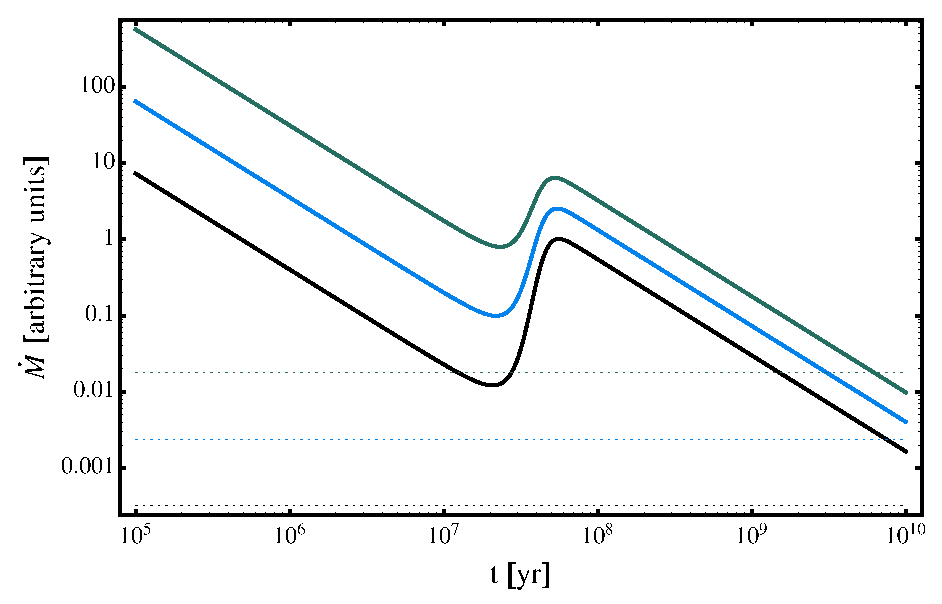
\includegraphics[width=\columnwidth]{NickPlot.eps}
% \caption{\label{NickPlot} SMBH feeding rates $\dot{M}=\eta(t) \times \Mstar(r_{\rm s})$, in arbitrary units.  The green, blue, and black curves are for galaxies with $\Gamma$ values of $0.1$, $0.5$, and $0.9$, respectively.  Solid curves represent impulsive-mode star formation, while dotted curves represent continuous-mode star formation. {\bf NCS: I think these old continuous curves are wrong, need to revise}}
% \end{figure}

% In Fig. \ref{NickPlot} we plot $\dot{M}$, in arbitrary units, as a
% function of time, for three different stellar density profiles $\Gamma
% = \{1.1, 1.5, 1.9\}$ (which are normalized to have the same mass at an
% influence radius $r _{\rm soi}=10~{\rm pc}$ around a $10^7M_\odot$
% SMBH).  We parametrize the wind velocity as
% \begin{equation} \frac{v_{\rm w}}{3000 ~\rm
% km~s^{-1}}=520-495\tanh\left( \frac{t-10^{7.5}~{\rm yr}}{10^{7}~{\rm
% yr}}\right). \label{NickV1}
% \end{equation} This counts Type II SNe heating as ``winds;'' if
% instead we are in the portion of parameter space where $r_{\rm II}$ is
% very large, then we use the alternate parametrization
% \begin{equation} \frac{v_{\rm w}}{3000 ~\rm
% km~s^{-1}}=520-495\tanh\left( \frac{t-10^{7}~{\rm yr}}{10^{6.5}~{\rm
% yr}}\right), \label{NickV2}
% \end{equation} which only allows short lived Wolf-Rayet stars to
% contribute to the high-heating mode.  The ``impulsive burst'' mode of
% star formation produces large ($\sim 10$) differences between the
% three $\dot{M}$ curves at early times, when $r_{\rm s}$ is small, but
% smaller ($\sim 3$) differences at late times, when $r_{\rm s}$ is
% large.  We also plot, as dotted curves, a simple model for the
% ``continuous'' mode of star formation, where mass loss is calculated
% as $\bar{\eta} = \int\eta(t)dt/t_{\rm h} \approx 4$ and an average
% energy injection in the wind is calculated as $\bar{v_{\rm
% w}^2}=\int\eta(t)v_{\rm w}^2(t)dt/\bar{\eta} \approx (800~{\rm
% km~s}^{-1})^2$.  Interestingly, the continuous mode of star formation
% produces small differences from late-time $\dot{M}$ seen in cusp
% galaxies with impulsive star formation; however, continuous mode star
% formation decreases late-time $\dot{M}$ by an order of magnitude
% relative to impulsive star formation in core galaxies.  {\bf NCS: I
% think this old discussion of MDot in the continuous limit is wrong,
% need to revise}

The energy and mass injection from stellar winds will be the sum ofthe
contributions from main sequence and post-main sequence (PMS) stars.
For an impulsively formed stellar population of age $t$, the mass
injection rate per unit stellar mass,$\dot{\bar{m}}(t)$, and  the energy
injection rate per unit stellar mass, $\dot{\bar{e}}(t)$,  will be given by

\begin{align} 
  \dot{\bar{m}}(t) &= \frac{\Delta M(t) \mu(M_{\rm TO}(t))
    \left|\dot{M}_{\rm TO}(t)\right| + f_{\rm MS} \int_{m_0}^{m_{\rm
        T}(t)}
    \dot{m}(\Mstar, t) \mu(\Mstar) {\rm d}\Mstar }{\bar{m}_*}\\
  \dot{\bar{e}}(t) &=\dot{e}_{\rm TO}(t)+ f_{\rm MS} \int_{m_0}^{m_{\rm T}(t)}
  \frac{\vw^2(\Mstar, t) \dot{m}(\Mstar, t) \mu(\Mstar) {\rm d}\Mstar}{\bar{m}_*}.
  \label{eq:edotImp}
\end{align} 

The first terms in each expression above correspond to the
contributions from PMS stars, while the second terms correspond to the
contributions from main sequence stars. The main sequence winds are a
small fraction of the mass, and they may be not be thermalized and
mixed with the rest of the injected gas. Thus, we include a
thermalization efficiency, $ 0\le f_{\rm MS}\le 1$, in
equation~\eqref{eq:edotImp}. Throughout this paper we set $f_{\rm
  MS}=1$. 

We assume a Salpeter IMF $\mu(\Mstar)\sim M^{-2.35}$, truncated at $0.1
\Msun$ on the low mass end and at $100 \Msun$ on the high mass
end. The corresponding mean stellar mass, $\bar{m}_*$ is 0.35 $\Msun$.

For the turnoff mass, $M_{\rm TO}$, we take the following fitting
formula 

\begin{align}
\log(M_{\rm TO})=0.24 + 0.068 x^2-0.34 x+4.76 e^{-4.58 x},
\end{align}

where $x=\log(t/10^9 {\rm years})$ and $M_{\rm TO}$ is in units
$\Msun$. This fit is designed to reproduce the results in 
Table 9 of \citet{MaederMeynet:1987a} and then asymptotes to the fit
for $M_{\rm TO}$ given in equation (9) of \citet{CiottiOstriker:2007a}
for intermediate and late times ($t \gsim 10^8$ years).

For $\Delta M(t)$ we use equation (10) from \citet{CiottiOstriker:2007a}

\begin{align}
\Delta M=
\begin{cases}
0.945 M_{\rm TO}-0.503 & M_{\rm TO} < 9 \Msun\\
 M_{\rm TO}-1.4 \Msun &  M_{\rm TO} \ge 9 \Msun
\end{cases}
\end{align}

To estimate the mass loss from main sequence stars
$\dot{m}(\Mstar, t)$,
we use equation 4 \citet{SchroderCuntz:2005a}\footnote{This
  prescription is a generalization of the Reimers' mass loss law. This
expression is derived assuming the stellar wind results from the
turbulent overflow of moaterial in the chromosphere or underneath it.} {\bf AG:
  unfortunately this is not really meant for MS stars...}

\begin{align}
  \dot{m}(\Mstar)=8 \times 10^{-14} \frac{L_* R_*}{\Mstar}
  \left(\frac{T_{\rm eff}}{\rm 4000 K}\right)^{3.5}
  \left(1+\frac{g_{\odot}}{4300 g_*}\right) \Msun \pyear,\
\end{align}

where  $R_*$, $L_*$, $T_{\rm eff}$ and $g_*$ are the stellar radius,
luminosity, effective and surface gravity respectively. $g_{\odot}$ is
the stellar surface gravity. To calculate $R_*$ and $L_*$ we use the
following scaling relations (taken from Kippenhann and Weygert Figures
22.2 and 22.3).

\begin{align}
L_*=
\begin{cases}
L_{\odot} (\Mstar/\Msun)^{3.2} & \Mstar > \Msun \\
L_{\odot} (\Mstar/\Msun)^{2.5} & \Mstar \le \Msun
\end{cases}
\end{align}

\begin{align}
r_*=
\begin{cases}
R_{\odot} (\Mstar/\Msun)^{0.57} & \Mstar > \Msun \\
R_{\odot} (\Mstar/\Msun)^{0.8} & \Mstar \le \Msun
\end{cases}
\end{align}


To get a handle on $\dot{e}_{\rm TO}(t)$, we use the results from
\citet{VossDiehl+:2009a} who use a population synthesis code to
simulate the mass and energy injection into the ISM from an OB
association. For the first $\sim 10$ Myr the energy injection will
come from energetic Wolf-Rayet star winds. The energy injection rate
per massive star ($\Mstar>8 \Msun$), $\dot{\mathcal{E}} (t)$, from
stellar winds is plotted in the top panel of their Figure 7 and is
well fit {\bf AG: A little more detail here...} by

\begin{align}
\dot{\mathcal{E}} (t)=
\begin{cases}
  1.3 \times 10^{36} {\rm ergs/s} & t<4 \times 10^6 {\rm years}\\
  1.3  \times 10^{36} {\rm ergs/s} \left(\frac{t}{4 \times  10^6}\right)^{-3.73} & t \ge 4 \times 10^6 {\rm years}.
\end{cases}
\label{eq:voss}
\end{align}

 $\dot{e}_{\rm TO}(t)$ is related to $\dot{\mathcal{E}}$  via 

\begin{align}
\dot{e}_{\rm TO}(t)=f_{8} \dot{\mathcal{E}} / \bar{m}_*,
\label{eq:eto}
\end{align}

where $f_{8}$ is the fraction of the stellar population with
$\Mstar>8 \Msun$. $f_8=2.6 \times 10^{-3}$ for our assumed Salpeter
IMF.  Equation~\eqref{eq:voss} and~\eqref{eq:eto} will be valid onlyfor $t
\lsim 10$ Myr. However, the turnoff contribution will become extremely
energetically subdominant at later times as far slower dust-driven
winds come to dominate the energy budget {\bf AG: Nick check--is the
  preceding sentence accurate}

We calculate the wind velocity for main sequence winds $v_w (\Mstar,
t)$ using...{\bf AG:Current just use the value for the sun~430 km/s
  replace with the real prescription we end up using.}

The effective wind velocity in the impulsive limit may then be written
as 

\begin{align}
\bar{v}_w(t)=2 \dot{\bar{e}}(t)/\dot{\bar{m}}(t)
\label{eq:vwImp}
\end{align}

We plot $\bar{v}_w$ in Figure~\ref{fig:vwImp}.

\begin{figure}
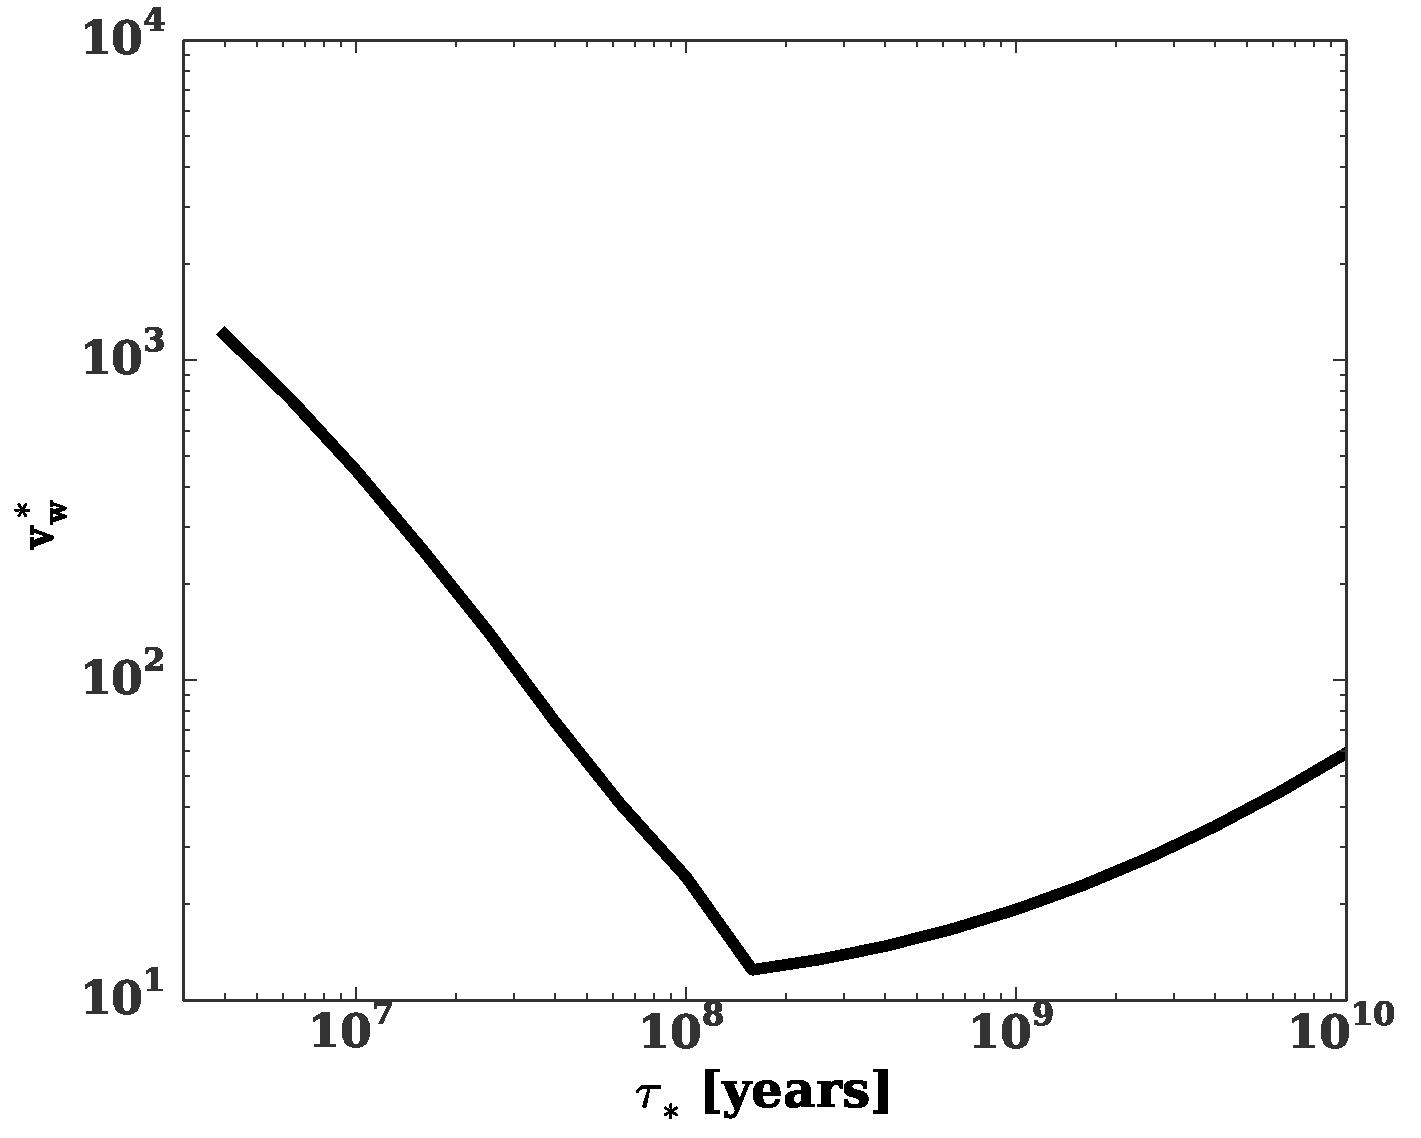
\includegraphics[width=\columnwidth]{vwImp.pdf}
\caption{\label{fig:vwImp} The effective $\vw$ from stellar winds from
  a stellar population formed in a starburst $t$ years ago.}
\end{figure}

We can then use these integrated quantities to determine the effective
$V_w$ for arbitrary star formation histories. For a stellar population
with star formation rate $S(t)$ 

\begin{align} 
  \dot{M}(t) &= \int_0^t S(t_1) \dot{\bar{m}}(t-t_1){\rm
      d}t_1\\
  \dot{E}(t) &= \int_0^t S(t_1) \dot{\bar{e}}(t-t_1){\rm
      d}t_1\\
  V_w^2(t) &=2 \dot{E}(t)/\dot{M}(t)
\end{align}

\begin{figure}
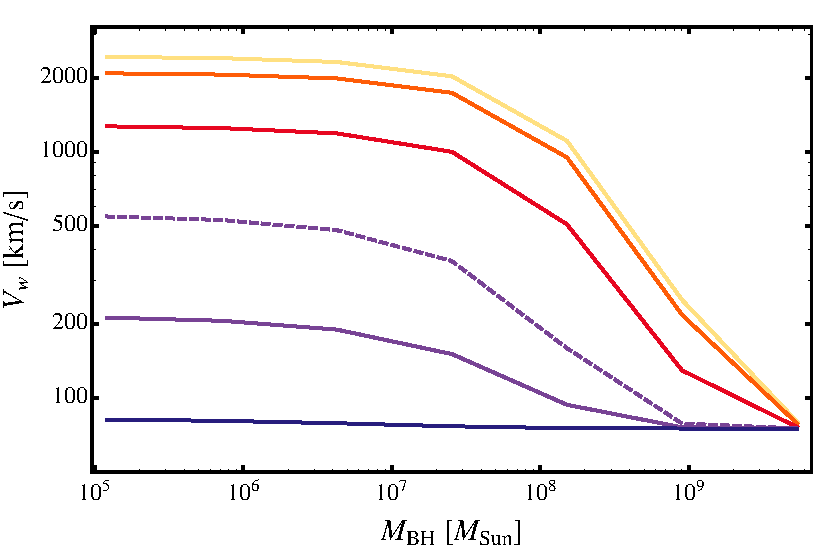
\includegraphics[width=\columnwidth]{vw.pdf}
\caption{\label{NickPlot2} Effective wind velocities $V_{\rm w}$ for
different $S(t)$.  The yellow and orange curves are the Moster SF
histories, with and without Type II SNe, respectively.  The red,
purple, and blue curves are Moster SFs convolved with a $\sin^2(t)$
function normalized to $10^7$, $10^8$, and $10^9$ yr fluctuations,
respectively.  These solid curves lack SN, but the dashed purple curve
possesses it.  Effective $V_{\rm w}$ is strongly diminished when the
variability timescale is greater than $\sim$ twice the duration of
high-velocity winds.}
\end{figure}

We show $V_{\rm W}$ for different star formation histories in
Fig. \ref{NickPlot2}.  In particular, we use Eqs. 17-20 from Moster et
al and the $M_{\rm BH}-M_{\rm halo}$ relation from Bandara et al {\bf
(NCS: add real refs)} to define $S(t)$ for particular galaxies.  It
seems that ``bumpy'' SF histories severely diminish $V_{\rm w}$ if the
timescale for SF variability is a factor of a few or more greater than
the duration of high-velocity winds (either 10 or 40 Myr).

%%% Local Variables: 
%%% mode: latex
%%% TeX-master: "ms"
%%% End: 


  \footnotesize{
    \bibliographystyle{mn2e}
    \bibliography{master}
  }
\end{document}
